% Options for packages loaded elsewhere
\PassOptionsToPackage{unicode}{hyperref}
\PassOptionsToPackage{hyphens}{url}
\PassOptionsToPackage{dvipsnames,svgnames,x11names}{xcolor}
%
\documentclass[
  letterpaper,
  DIV=11,
  numbers=noendperiod,
  oneside]{scrreprt}

\usepackage{amsmath,amssymb}
\usepackage{iftex}
\ifPDFTeX
  \usepackage[T1]{fontenc}
  \usepackage[utf8]{inputenc}
  \usepackage{textcomp} % provide euro and other symbols
\else % if luatex or xetex
  \usepackage{unicode-math}
  \defaultfontfeatures{Scale=MatchLowercase}
  \defaultfontfeatures[\rmfamily]{Ligatures=TeX,Scale=1}
\fi
\usepackage{lmodern}
\ifPDFTeX\else  
    % xetex/luatex font selection
\fi
% Use upquote if available, for straight quotes in verbatim environments
\IfFileExists{upquote.sty}{\usepackage{upquote}}{}
\IfFileExists{microtype.sty}{% use microtype if available
  \usepackage[]{microtype}
  \UseMicrotypeSet[protrusion]{basicmath} % disable protrusion for tt fonts
}{}
\makeatletter
\@ifundefined{KOMAClassName}{% if non-KOMA class
  \IfFileExists{parskip.sty}{%
    \usepackage{parskip}
  }{% else
    \setlength{\parindent}{0pt}
    \setlength{\parskip}{6pt plus 2pt minus 1pt}}
}{% if KOMA class
  \KOMAoptions{parskip=half}}
\makeatother
\usepackage{xcolor}
\usepackage[left=1in,marginparwidth=2.0666666666667in,textwidth=4.1333333333333in,marginparsep=0.3in]{geometry}
\setlength{\emergencystretch}{3em} % prevent overfull lines
\setcounter{secnumdepth}{5}
% Make \paragraph and \subparagraph free-standing
\ifx\paragraph\undefined\else
  \let\oldparagraph\paragraph
  \renewcommand{\paragraph}[1]{\oldparagraph{#1}\mbox{}}
\fi
\ifx\subparagraph\undefined\else
  \let\oldsubparagraph\subparagraph
  \renewcommand{\subparagraph}[1]{\oldsubparagraph{#1}\mbox{}}
\fi


\providecommand{\tightlist}{%
  \setlength{\itemsep}{0pt}\setlength{\parskip}{0pt}}\usepackage{longtable,booktabs,array}
\usepackage{calc} % for calculating minipage widths
% Correct order of tables after \paragraph or \subparagraph
\usepackage{etoolbox}
\makeatletter
\patchcmd\longtable{\par}{\if@noskipsec\mbox{}\fi\par}{}{}
\makeatother
% Allow footnotes in longtable head/foot
\IfFileExists{footnotehyper.sty}{\usepackage{footnotehyper}}{\usepackage{footnote}}
\makesavenoteenv{longtable}
\usepackage{graphicx}
\makeatletter
\def\maxwidth{\ifdim\Gin@nat@width>\linewidth\linewidth\else\Gin@nat@width\fi}
\def\maxheight{\ifdim\Gin@nat@height>\textheight\textheight\else\Gin@nat@height\fi}
\makeatother
% Scale images if necessary, so that they will not overflow the page
% margins by default, and it is still possible to overwrite the defaults
% using explicit options in \includegraphics[width, height, ...]{}
\setkeys{Gin}{width=\maxwidth,height=\maxheight,keepaspectratio}
% Set default figure placement to htbp
\makeatletter
\def\fps@figure{htbp}
\makeatother
\newlength{\cslhangindent}
\setlength{\cslhangindent}{1.5em}
\newlength{\csllabelwidth}
\setlength{\csllabelwidth}{3em}
\newlength{\cslentryspacingunit} % times entry-spacing
\setlength{\cslentryspacingunit}{\parskip}
\newenvironment{CSLReferences}[2] % #1 hanging-ident, #2 entry spacing
 {% don't indent paragraphs
  \setlength{\parindent}{0pt}
  % turn on hanging indent if param 1 is 1
  \ifodd #1
  \let\oldpar\par
  \def\par{\hangindent=\cslhangindent\oldpar}
  \fi
  % set entry spacing
  \setlength{\parskip}{#2\cslentryspacingunit}
 }%
 {}
\usepackage{calc}
\newcommand{\CSLBlock}[1]{#1\hfill\break}
\newcommand{\CSLLeftMargin}[1]{\parbox[t]{\csllabelwidth}{#1}}
\newcommand{\CSLRightInline}[1]{\parbox[t]{\linewidth - \csllabelwidth}{#1}\break}
\newcommand{\CSLIndent}[1]{\hspace{\cslhangindent}#1}

\KOMAoption{captions}{tableheading}
\makeatletter
\@ifpackageloaded{tcolorbox}{}{\usepackage[skins,breakable]{tcolorbox}}
\@ifpackageloaded{fontawesome5}{}{\usepackage{fontawesome5}}
\definecolor{quarto-callout-color}{HTML}{909090}
\definecolor{quarto-callout-note-color}{HTML}{0758E5}
\definecolor{quarto-callout-important-color}{HTML}{CC1914}
\definecolor{quarto-callout-warning-color}{HTML}{EB9113}
\definecolor{quarto-callout-tip-color}{HTML}{00A047}
\definecolor{quarto-callout-caution-color}{HTML}{FC5300}
\definecolor{quarto-callout-color-frame}{HTML}{acacac}
\definecolor{quarto-callout-note-color-frame}{HTML}{4582ec}
\definecolor{quarto-callout-important-color-frame}{HTML}{d9534f}
\definecolor{quarto-callout-warning-color-frame}{HTML}{f0ad4e}
\definecolor{quarto-callout-tip-color-frame}{HTML}{02b875}
\definecolor{quarto-callout-caution-color-frame}{HTML}{fd7e14}
\makeatother
\makeatletter
\makeatother
\makeatletter
\@ifpackageloaded{bookmark}{}{\usepackage{bookmark}}
\makeatother
\makeatletter
\@ifpackageloaded{caption}{}{\usepackage{caption}}
\AtBeginDocument{%
\ifdefined\contentsname
  \renewcommand*\contentsname{Tabla de contenidos}
\else
  \newcommand\contentsname{Tabla de contenidos}
\fi
\ifdefined\listfigurename
  \renewcommand*\listfigurename{Listado de Figuras}
\else
  \newcommand\listfigurename{Listado de Figuras}
\fi
\ifdefined\listtablename
  \renewcommand*\listtablename{Listado de Tablas}
\else
  \newcommand\listtablename{Listado de Tablas}
\fi
\ifdefined\figurename
  \renewcommand*\figurename{Figura}
\else
  \newcommand\figurename{Figura}
\fi
\ifdefined\tablename
  \renewcommand*\tablename{Tabla}
\else
  \newcommand\tablename{Tabla}
\fi
}
\@ifpackageloaded{float}{}{\usepackage{float}}
\floatstyle{ruled}
\@ifundefined{c@chapter}{\newfloat{codelisting}{h}{lop}}{\newfloat{codelisting}{h}{lop}[chapter]}
\floatname{codelisting}{Listado}
\newcommand*\listoflistings{\listof{codelisting}{Listado de Listados}}
\makeatother
\makeatletter
\@ifpackageloaded{caption}{}{\usepackage{caption}}
\@ifpackageloaded{subcaption}{}{\usepackage{subcaption}}
\makeatother
\makeatletter
\@ifpackageloaded{tcolorbox}{}{\usepackage[skins,breakable]{tcolorbox}}
\makeatother
\makeatletter
\@ifundefined{shadecolor}{\definecolor{shadecolor}{rgb}{.97, .97, .97}}
\makeatother
\makeatletter
\makeatother
\makeatletter
\@ifpackageloaded{sidenotes}{}{\usepackage{sidenotes}}
\@ifpackageloaded{marginnote}{}{\usepackage{marginnote}}
\makeatother
\makeatletter
\makeatother
\ifLuaTeX
\usepackage[bidi=basic]{babel}
\else
\usepackage[bidi=default]{babel}
\fi
\babelprovide[main,import]{spanish}
% get rid of language-specific shorthands (see #6817):
\let\LanguageShortHands\languageshorthands
\def\languageshorthands#1{}
\ifLuaTeX
  \usepackage{selnolig}  % disable illegal ligatures
\fi
\IfFileExists{bookmark.sty}{\usepackage{bookmark}}{\usepackage{hyperref}}
\IfFileExists{xurl.sty}{\usepackage{xurl}}{} % add URL line breaks if available
\urlstyle{same} % disable monospaced font for URLs
\hypersetup{
  pdftitle={Introducción a la estadística industrial y la ciencia de datos utilizando Microsoft Excel y R},
  pdfauthor={Juan Riera},
  pdflang={es},
  colorlinks=true,
  linkcolor={blue},
  filecolor={Maroon},
  citecolor={Blue},
  urlcolor={Blue},
  pdfcreator={LaTeX via pandoc}}

\title{Introducción a la estadística industrial y la ciencia de datos
utilizando Microsoft Excel y R}
\usepackage{etoolbox}
\makeatletter
\providecommand{\subtitle}[1]{% add subtitle to \maketitle
  \apptocmd{\@title}{\par {\large #1 \par}}{}{}
}
\makeatother
\subtitle{Manual para la Formación Profesional}
\author{Juan Riera}
\date{12/12/22}

\begin{document}
\maketitle
\ifdefined\Shaded\renewenvironment{Shaded}{\begin{tcolorbox}[frame hidden, boxrule=0pt, enhanced, interior hidden, borderline west={3pt}{0pt}{shadecolor}, sharp corners, breakable]}{\end{tcolorbox}}\fi

\renewcommand*\contentsname{Tabla de contenidos}
{
\hypersetup{linkcolor=}
\setcounter{tocdepth}{2}
\tableofcontents
}
\bookmarksetup{startatroot}

\hypertarget{prefacio}{%
\chapter*{Prefacio}\label{prefacio}}
\addcontentsline{toc}{chapter}{Prefacio}

\markboth{Prefacio}{Prefacio}

Este libro trata sobre la enseñanza de algunos métodos básicos de la
estadística y la moderna ciencia de datos y su aplicación al entorno
industrial. Está concebido de forma práctica con multitud de ejemplos,
no sólo industriales, con el objetivo de mostrar los métodos
cuantitativos de análisis, y también el razonamiento necesario para dar
sentido a los resultados presentados por las herramientas de análisis de
datos.

El objetivo del libro es acercar a los estudiantes de la Formación
Profesional al uso de las herramientas de análisis de datos
industriales. El entorno de la industria 4.0 produce un enorme y
constante flujo de datos como resultado tanto de la implantación de
sistemas de captura automáticos como del aumento de la tecnificación de
los puestos de trabajo; se requiere por parte de los profesionales
industriales que sean capaces de analizar esta enorme cantidad de datos
para transformarlos en información para la decisión. En la empresa
industrial actual, son los ingenieros y técnicos de planta, y no
estadísticos o ingenieros informáticos, quienes participan diariamente
en la presentacion y discusion de los datos y en la toma de decisiones
operativas, tanto en los equipos de trabajo como ante la Dirección. Por
esta razón, considero necesario proporcionar a los estudiantes de la
Formación Profesional un conocimiento suficiente de los conceptos,
herramientas y métodos del análisis de datos, así como de las técnicas
básicas de presentación y comunicación de la información.

El control estadístico de la calidad empezó con W.E. Deming a mediados
del pasado siglo XX, y fueron las empresas japonesas, sobre todo las
automovilísticas, las que inicialmente recogieron el testigo de Deming y
aplicaron estos principios a la mejora de la producción industrial,
difundiendo su conocimiento a todos los niveles jerárquicos de las
organizaciones, desde los operarios de línea hasta los más altos
directivos. Desde ese momento hasta la difusión actual de los métodos
Six Sigma gracias a General Electric y Motorola, la mejora industrial de
los procesos ha estado siempre apoyada en la correcta utilización de
estas metodologías.

La enseñanza de los conceptos estadísticos está, casi siempre, a cargo
de profesores con una gran formación en matemáticas. Estos profesores
suelen identificar la comprensión de los conceptos estadísticos con su
comprensión matemática. Sin embargo, cuando enseñamos estadística
industrial, debemos hacer énfasis tanto en las ideas y la comprensión de
los conceptos como en su utilización práctica, y reconocer que el
razonamiento matemático no es el único camino para la comprensión
conceptual.

La práctica de la estadística requiere buen juicio y sentido común. Dado
que el buen juicio se desarrolla con la experiencia, un curso de
iniciación debe presentar unas guías claras de aplicación de los
métodos, y no dar por supuestas unas exigencias excesivamente altas
sobre la capacidad de juicio analítico de los estudiante; no sería un
planteamiento razonable. Con el fin de desarrollar esta capacidad de
juicio analítico he introducido explicaciones detalladas en la mayor
parte de los ejemplos. En todos los casos, los ejercicios requerirán del
estudiante no sólo una resolución numérica, sino el uso del juicio
analítico y la explicación verbal (o escrita) de las decisiones tomadas
y conclusiones realizadas. Creo que este planteamiento será mucho más
beneficioso a largo plazo que limitarse a una simple resolución
numérica.

Mi experiencia industrial me ha mostrado que en las situaciones reales,
sobre el terreno, la comprensión práctica de los conceptos es más
importante que su rigurosa formulación matemática. Por esta razón, en el
desarrollo del contenido del libro he insistido más en la forma de
aplicar las herramientas y entender los análisis que en el conocimiento
formal de las fórmulas estadísticas y su deducción matemática. He hecho
especial hincapié en la utilización de herramientas sencillas, sobre
todo gráficas, que casi siempre son una ayuda para comprender la
información contenida en un conjunto de datos. El objetivo es
proporcionar al estudiante las bases de la metodología del análisis de
datos y del análisis estadístico, y cómo puede aplicarse a la resolución
de problemas técnicos concretos, más que el conocimiento de la teoría
matemática de la estadística.

He evitado las explicaciones formales sobre temas estadísticos cuando no
son indispensables para su aplicación práctica. Así, por ejemplo, al
explicar la media de un conjunto de datos considero más importante
entender el concepto físico de ``centro de gravedad'' que los conceptos
estadísticos de esperanza matemática, que no se tocan en este texto. En
este sentido, he intentado que el alumno aprenda a diferenciar ``en qué
consiste'' un estadístico, de ``cómo se calcula''. Comprender la
diferencia entre el concepto y su fórmula de cálculo es fundamental para
entender en qué situación debe usarse uno u otro estadístico.

\begin{figure}

\begin{minipage}[b]{0.50\linewidth}

{\centering 

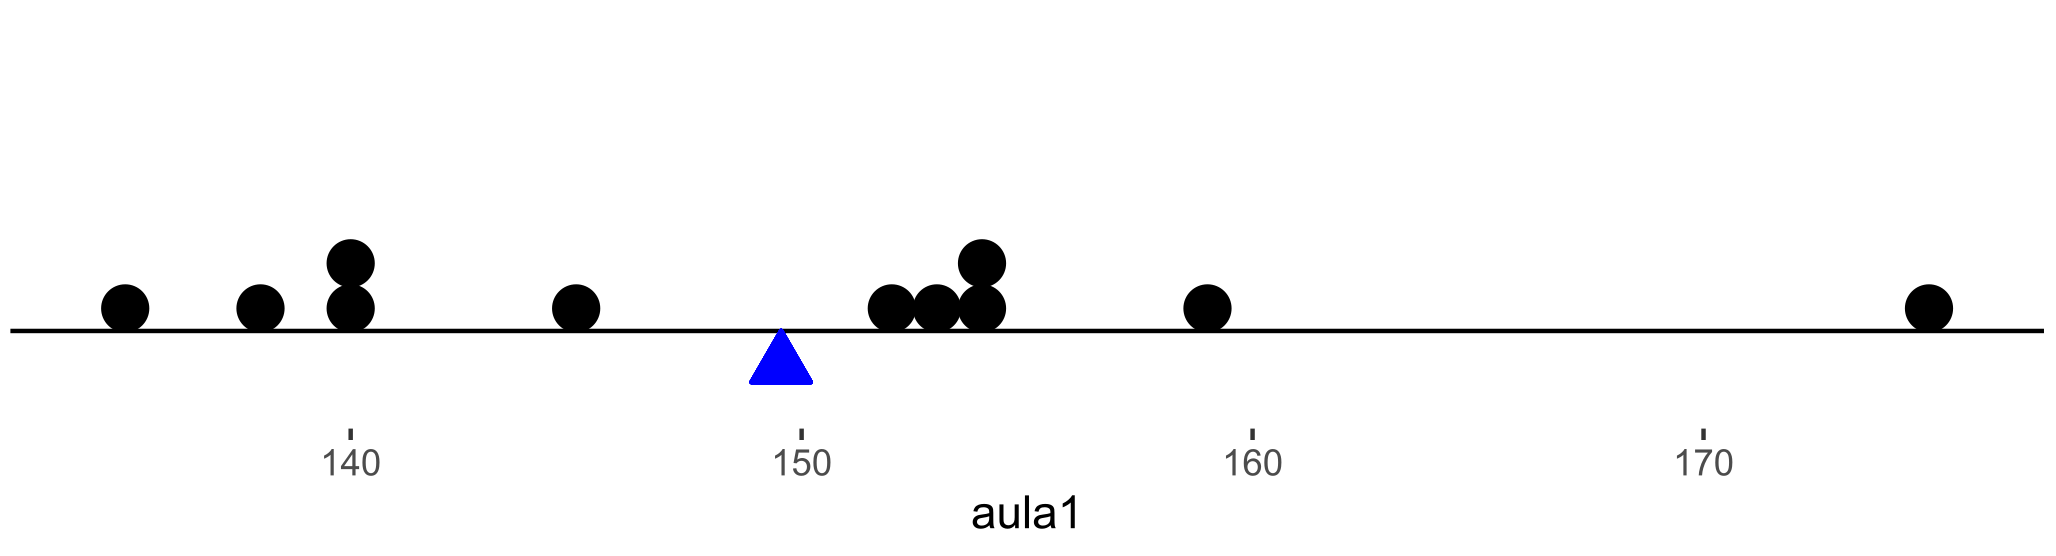
\includegraphics{index_files/mediabag/01-imagenes/media-balanza.pdf}

}

\subcaption{\label{fig-media}Diagrama de puntos (dotplot) mostrando la
posición de la media}
\end{minipage}%
%
\begin{minipage}[b]{0.50\linewidth}

{\centering 

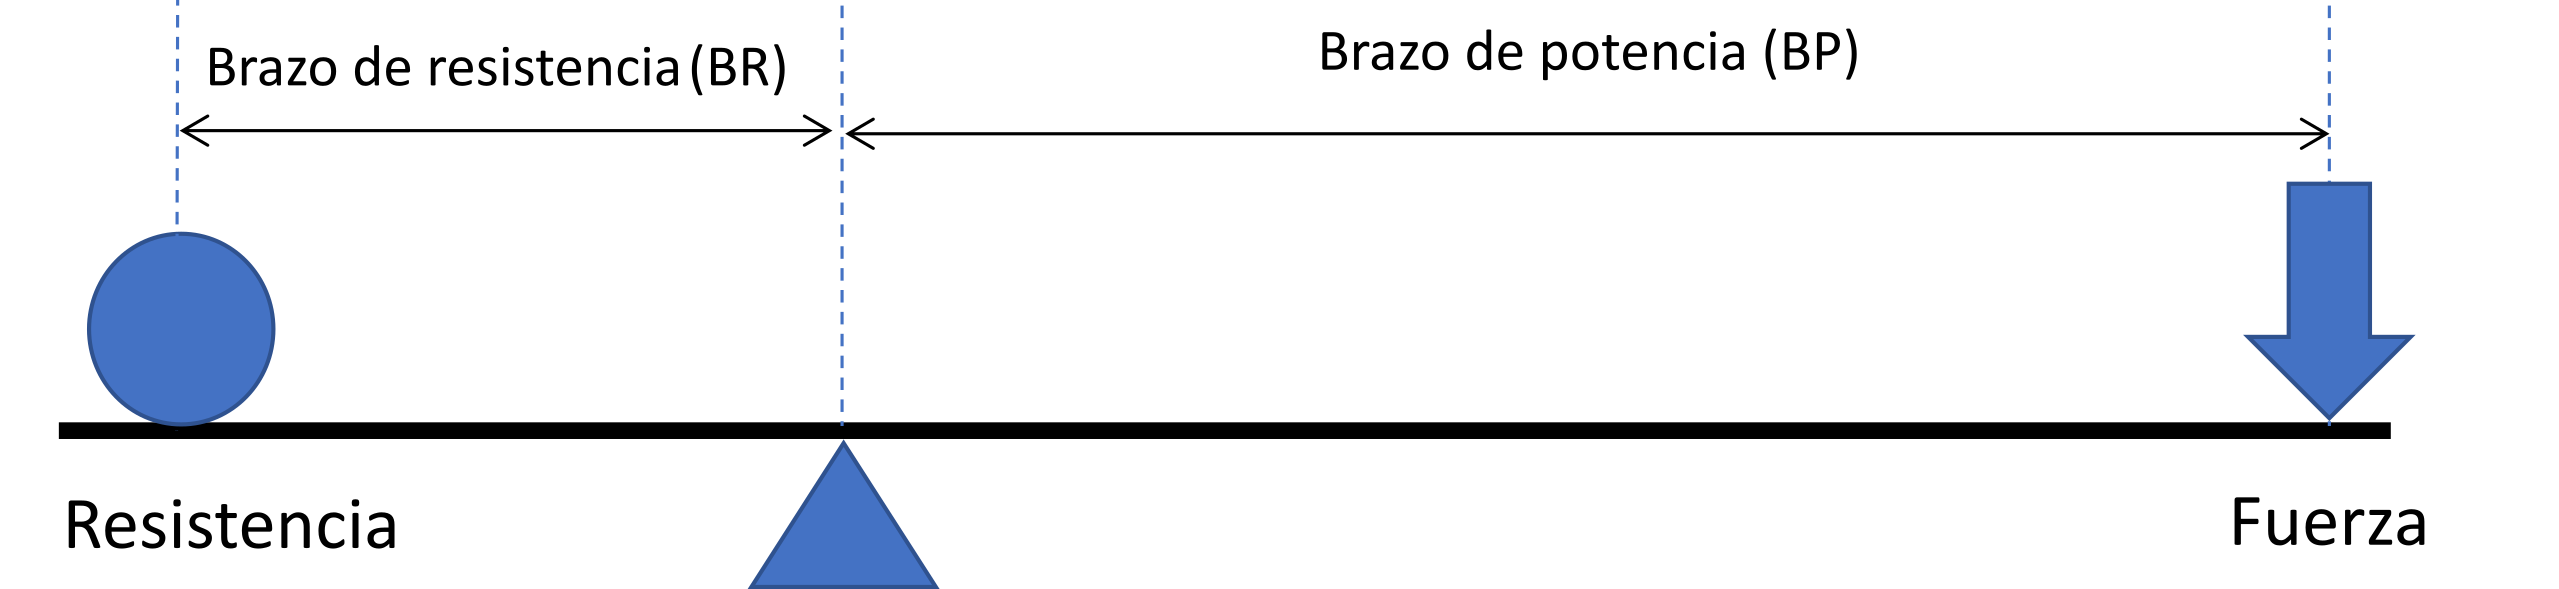
\includegraphics{01-imagenes/palanca.png}

}

\subcaption{\label{fig-palanca}Palanca de primer grado con el fulcro
como punto de equilibrio}
\end{minipage}%

\caption{\label{fig-intro-media}Comparación gráfica del significado de
la media en un diagrama de puntos (\emph{dotplot}) con una palanca de
primer grado.}

\end{figure}

Un curso de introducción a la estadística y análisis de datos
industriales debe ser ante todo práctico y orientado a su aplicación en
el entorno industrial real. Los principales temas de trabajo estadístico
en la industria tienen que ver con la captura de datos, su
almacenamiento y su depuración, su descripción utilizando gráficos, la
inferencia (intervalos de confianza y tests), la construcción de modelos
explicativos, el diseño de los experimentos industriales, el control
estadístico de la calidad y la exposición y presentación de resultados.
Dado el alcance limitado de este libro, algunos de estos temas se
tratarán de forma muy ligera, y necesitarán de un estudio posterior si
el alumno tiene interés en profundizar en ellos. A pesar de que los
temas más especializados puedan ser importantes en algunas aplicaciones
específicas, no preparan al estudiante para lo que se va a encontrar en
el terreno en la mayor parte de las ocasiones. En cambio, la resolución
de problemas en equipo en un entorno de aprendizaje dinámico
enfrentándose a problemas exigentes, y el desarrollo de las habilidades
de análisis, de síntesis y de comunicación, tendrán un impacto mucho más
positivo.

He intentado mostrar la necesidad de que los estudiantes comprendan y
apliquen el método científico en el entorno industrial, y no sólo
apliquen un recetario de procedimientos de manera automática. Es mucho
mas importante la comprensión y adecuada utilización del método
científico y de las herramientas y gráficos básicos, antes que la
aplicación rutinaria y mecánica de determinadas fórmulas matemáticas o
métodos sofisticados y complejos que el alumno puede no comprender en
toda su profundidad.

Las industrias líderes destacan por la aplicación intensiva de métodos
sofisticados, tales como Six Sigma, Lean Manufacturing, diseño robusto
de productos, y otros que hacen un uso intensivo de los datos, tanto de
los obtenidos en producción como de los obtenidos en la realización de
experimentos bien diseñados. La mejora de la competitividad en estas
empresas no se debe tanto a la aplicación de unos u otros métodos, como
al desarrollo del juicio analítico de sus equipos y a la aplicación de
lo aprendido a la mejora continua de los procesos industriales. Veremos
que la experiencia y el conocimiento tecnológico de estos procesos son
fundamentales para el desarrollo del buen juicio analítico, y, en
consecuencia, para la buena interpretación de los resultados que se
obtienen con las herramientas estadísticas y de análisis.

Tratándose de un libro para el uso en la Formación Profesional,
considero prioritario que su estudio se oriente al desarrollo de
habilidades que sean de aplicación práctica directa en el puesto de
trabajo y además faciliten la empleabilidad del estudiante, y no a la
obtención de conocimiento abstracto. El
\href{https://www.weforum.org/publications/the-future-of-jobs-report-2023}{Informe
sobre el futuro del empleo}, publicado por el
\href{https://www.weforum.org/}{Foro Económico MUndial} en mayo de 2023,
considera que las principales habilidades clave en el trabajo del futuro
serán en primer lugar el desarrollo del pensamiento analítico y, en
segundo, del pensamiento crítico; unidas al desarrollo de la curiosidad
y la voluntad de aprendizaje a lo largo de la vida, la eficacia, la
confianza en el propio trabajo y la atención al detalle. La voluntad de
este libro es proporcionar conocimientos que ayuden al estudiante a
desarrollarse en esta dirección.

\hypertarget{a-quiuxe9n-va-dirigido-este-libro}{%
\section*{A quién va dirigido este
libro}\label{a-quiuxe9n-va-dirigido-este-libro}}
\addcontentsline{toc}{section}{A quién va dirigido este libro}

\markright{A quién va dirigido este libro}

El libro está orientado a completar la formación técnica de los
estudiantes de Formación Profesional, en las especialidades relacionadas
con la actividad productiva industrial. También creo que será de
utilidad para los técnicos industriales en activo que no han tenido una
adecuada formación en estas metodologías, y que han encontrado
dificultad para lanzarse a su aprendizaje mientras desarrollan so
actividad profesional. Espero, también, que los profesores de la
Formación Profesional en estos ámbitos de competencia encuentren en este
documento los elementos de apoyo que les permitan integrar estas
enseñanzas en sus respectivos ciclos formativos.

En todos los casos, el aprendizaje requerirá de un esfuerzo que quizás
será mayor en los estudiantes que no tengan una base mínima en álgebra y
cálculo. En estos casos, el trabajo en equipo y la discusión abierta
entre compañeros y con los profesores ayudará a la comprensión de los
conceptos.

\hypertarget{organizaciuxf3n-del-libro}{%
\section*{Organización del libro}\label{organizaciuxf3n-del-libro}}
\addcontentsline{toc}{section}{Organización del libro}

\markright{Organización del libro}

El \textbf{capítulo 1} proporciona una introducción general al
\textbf{pensamiento estadístico} y su aplicación industrial. Introduce
también algunos conceptos sobre la ética en análisis de datos y una
reflexión sobre la honestidad del investigador o analista. Se introduce
también el concepto actual de \textbf{repetibilidad} en la elaboración
de los informes estadísticos.

El \textbf{capítulo 2} presenta las principales herramientas que
usaremos en este libro para el análisis de los datos industriales,
concretamente Microsoft Excel y R.

El \textbf{capítulo 3} trata fundamentalmente de la forma de recoger los
datos y su almacenamiento. Introduce el concepto de \textbf{datos
ordenados} o \textbf{arreglados} (\emph{tidy data}), que resulta
fundamental para las fases posteriores de análisis.

En el \textbf{capítulo 4} se introducen los métodos básicos para resumir
tablas de datos y la \textbf{presentación mediante el uso de gráficos},
en lo que se conoce como \emph{exploración de datos}, que suele ser un
paso previo al análisis más detallado y a la formulación de hipótesis.

El \textbf{capítulo 5} introduce el concepto de \textbf{probabilidad},
así como las distribuciones de probabilidad, necesarias para la
construcción de los tests de hipótesis y, en general, de la estadística
inferencial. Este es un contenido que se presenta de forma breve y sobre
todo práctica.

En el \textbf{capítulo 6} se presentan los métodos para detectar la
\textbf{relación entre dos variables}, haciendo énfasis en los métodos
gráficos, y se discute las diferencias entre correlación y causalidad.

El \textbf{capítulo 7} introduce de manera sencilla el \textbf{análisis
de la varianza}, necesario para métodos importantes en la industria como
el control de la precisión analítica, que se trata en el capítulo
siguiente.

El \textbf{capítulo 8} trata del análisis del sistema de medición, la
calidad de las medidas y la medida de la precisión analítica. Resulta
sorprendente la cantidad de laboratorios que dan soporte analítico a
procesos productivos de gran impacto económico en la vida de la empresa,
sin realizar nunca un autocontrol sobre el nivel de precisión de sus
análisis. En este capítulo se hace una presentación básica del tema con
el objetivo de que resulte útil y práctica.

El \textbf{capítulo 9} presenta una de las aplicaciones más importantes
de la estadística en el entorno industrial, el \textbf{control
estadístico de procesos}. Dada la importancia de este capítulo, se
refuerza su contenido con numerosos ejemplos y casos prácticos, y se
incluye un caso extenso para su análisis.

En el \textbf{capítulo 10} se hace una introducción al \textbf{diseño de
experimentos}. La utilidad de esta técnica es primordial para el
industrial, sobre todo para el área de I+D y el diseño de productos.
Dado que esta técnica puede ser muy compleja en su aplicación real, se
facilitan enlaces a otros recursos, como cursos, que serán útiles a los
que quieran profundizar más.

Finalmente, en el \textbf{capítulo 11} se presenta el uso de los
conceptos y técnicas estudiadas en los procesos de mejora de la calidad
industrial, y se introducen algunas aplicaciones prácticas de la
estadística en el entorno industrial, como \textbf{Six Sigma}.

\hypertarget{cuxf3mo-usar-el-libro}{%
\section*{Cómo usar el libro}\label{cuxf3mo-usar-el-libro}}
\addcontentsline{toc}{section}{Cómo usar el libro}

\markright{Cómo usar el libro}

He intentado que cada capítulo sea lo más autocontenido posible de forma
que se facilite la organización pedagógica por temas. No obstante, hay
algunos contenidos que pueden necesitar contenidos de los capítulos
anteriores, por lo que se sugiere estudiarlo en el orden presentado.

El libro es eminentemente práctico, con numerosos ejercicios; su
resolución puede ser individual o en equipo.

Algunos recuadros utilizan códigos de color para indicar el objetivo de
la información que contienen. Básicamente, los colores utilizados son:

\begin{tcolorbox}[enhanced jigsaw, colback=white, opacitybacktitle=0.6, leftrule=.75mm, opacityback=0, coltitle=black, colframe=quarto-callout-note-color-frame, colbacktitle=quarto-callout-note-color!10!white, bottomrule=.15mm, title={Problema o cuestión a resolver}, bottomtitle=1mm, toptitle=1mm, breakable, left=2mm, arc=.35mm, titlerule=0mm, rightrule=.15mm, toprule=.15mm]

El recuadro azul se utilizará para proponer problemas sencillos cuya
respuesta se encuentra más adelante en el texto. El objetivo de estos
problemas es estimular la reflexión, aunque puede ser necesario recurrir
a cálculos sencillos ayudados por las herramientas disponibles.

\end{tcolorbox}

\begin{tcolorbox}[enhanced jigsaw, colback=white, opacitybacktitle=0.6, leftrule=.75mm, opacityback=0, coltitle=black, colframe=quarto-callout-tip-color-frame, colbacktitle=quarto-callout-tip-color!10!white, bottomrule=.15mm, title={Respuesta al problema o cuestión a resolver}, bottomtitle=1mm, toptitle=1mm, breakable, left=2mm, arc=.35mm, titlerule=0mm, rightrule=.15mm, toprule=.15mm]

El recuadro verde se utilizará para proponer una respuesta al problema
planteado; respuesta que no tiene por qué ser la única posible.
Normalmente se presentará de forma oculta.

\end{tcolorbox}

Además se incluyen diferentes tipos de avisos cada vez que se introduce
algún concepto que es necesario resaltar.

\begin{tcolorbox}[enhanced jigsaw, colback=white, opacitybacktitle=0.6, leftrule=.75mm, opacityback=0, coltitle=black, colframe=quarto-callout-important-color-frame, colbacktitle=quarto-callout-important-color!10!white, bottomrule=.15mm, title=\textcolor{quarto-callout-important-color}{\faExclamation}\hspace{0.5em}{Importante}, bottomtitle=1mm, toptitle=1mm, breakable, left=2mm, arc=.35mm, titlerule=0mm, rightrule=.15mm, toprule=.15mm]

En este formato se indican cuestiones importantes

\end{tcolorbox}

\begin{tcolorbox}[enhanced jigsaw, colback=white, opacitybacktitle=0.6, leftrule=.75mm, opacityback=0, coltitle=black, colframe=quarto-callout-warning-color-frame, colbacktitle=quarto-callout-warning-color!10!white, bottomrule=.15mm, title=\textcolor{quarto-callout-warning-color}{\faExclamationTriangle}\hspace{0.5em}{¡Atención!}, bottomtitle=1mm, toptitle=1mm, breakable, left=2mm, arc=.35mm, titlerule=0mm, rightrule=.15mm, toprule=.15mm]

En este formato se indican cuestiones a las que hay que prestar especial
atención o que pueden inducir a error

\end{tcolorbox}

\hypertarget{uso-del-ordenador-y-el-software-estaduxedstico}{%
\section*{\texorpdfstring{Uso del ordenador y el \emph{software}
estadístico}{Uso del ordenador y el software estadístico}}\label{uso-del-ordenador-y-el-software-estaduxedstico}}
\addcontentsline{toc}{section}{Uso del ordenador y el \emph{software}
estadístico}

\markright{Uso del ordenador y el \emph{software} estadístico}

En la práctica diaria, los técnicos industriales usan los ordenadores
para almacenar y visualizar los datos de producción, para solucionar
problemas mediante análisis estadísticos, y para presentar sus
resultados de forma gráfica. De la misma forma que en el entorno
industrial, en este libro se utilizarán también los ordenadores de forma
habitual, y por esta razón es imprescindible que los estudiantes tengan
acceso individual a un ordenador en el que esté instalado el software
recomendado, y que se acostumbren a utilizarlo para resolver los
problemas y casos planteados como ejercicios prácticos, individualmente
y en grupo.

El estudiante que se incorpora a una empresa, sea en un laboratorio o en
una planta de producción, se va a encontrar muy pronto delante de una
hoja de cálculo, y debe saber cómo utilizarla correctamente.
Actualmente, lo más probable es que esa hoja de cálculo sea Microsoft
Excel, aunque hay otras alternativas posibles, como Google Sheets, Apple
Numbers, OpenOffice Calc y algunas más. La gran dominancia en el mercado
de Microsoft Excel ha hecho que todas estas herramientas sean totalmente
compatibles o tengan modos de compatibilidad con Excel. Por esta razón,
este libro se basa en la utilización de Excel como hoja de cálculo y
herramienta principal para el almacenamiento de datos.

A lo largo del libro se presentarán informes y gráficos obtenidos con
Microsoft Excel, y también con el
\href{https://en.wikipedia.org/wiki/R_\%28programming_language\%29}{software
estadístico R}. Prácticamente todos ellos pueden ser exportados a otras
herramientas, como Google Sheets, OpenOffice, Minitab o Matlab, o
analizarse con otros lenguajes de programación, como Python o Julia. En
realidad, el método de análisis y cómo obtener un resultado correcto son
aspectos más importantes que la herramienta que se utilice para ello,
por lo que queda en manos del instructor la decisión final sobre qué
usar y cómo. Para facilitar este trabajo de conversión, en su caso, todo
el material del libro y los datos de ejemplo estarán disponibles en un
repositorio de GitHub.

Algunos ejercicios tienen que ver con la interpretación y presentación
de los resultados. Es importante que estos trabajos se realicen en grupo
y se haga énfasis en la comprensión del problema y en su correcta
exposición; en los equipos industriales de hoy, la discusión de
problemas y la exposición de resultados, en reuniones de trabajo o en
paneles informativos a pie de planta, forma parte del trabajo diario.
Estas habilidades de comunicación deben ser desarrolladas en los
estudiantes de forma prioritaria.

La ventaja de R sobre Excel es que el código R, si está bien
documentado, muestra cada paso realizado, y esto permite que otras
personas puedan verificar el resultado y reproducirlo a partir de los
datos originales, e incluso reutilizar los procedimientos. Utilizar
código en vez de clicks de ratón es esencial para asegurar la
\textbf{reproducibilidad de los análisis de datos}\footnote{El concepto
  de reproducibilidad, cada vez más importante, se desarrolla en el
  capítulo 2}. Por esta razón, recomiendo el uso del lenguaje R como
complemento o alternativa a la hoja de cálculo, tanto para analizar como
para visualizar datos. Sin embargo, como la realidad del mundo de la
empresa es que los lenguajes como R están todavía poco introducidos, es
inevitable mantener el uso de la hoja de cálculo; en el libro se
explicarán algunas \emph{mejores prácticas}, que permitirán el uso
simultáneo de ambas herramientas de forma óptima.

Respecto a la \textbf{programación informática}, en el libro no se hace
énfasis en la programación R más que como sucesión de órdenes
individuales en scripts sencillos. No se busca la eficiencia
computacional ni la rapidez en el cálculo, sino la comprensión de la
metodología de resolución de problemas y cómo ésta se apoya en las
herramientas presentadas. De la misma manera, tampoco se hace ningún uso
de la programación en Excel, ya sea con \textbf{macros} o con
\textbf{Visual Basic}; estos temas quedan fuera del perímetro de este
libro.

Un paso en la dirección de la implantación de \textbf{flujos de trabajo
reproducibles} es la elaboración de informes automatizados. Estos
informes incluyen el código R, los comentarios del autor en forma de
texto formateado en
\href{https://es.wikipedia.org/wiki/Markdown}{\emph{markdown}}, y los
resultados del código. Herramientas como
\href{https://quarto.org/}{Quarto}, o
\href{https://colab.research.google.com/}{Google Colaboratory}, que usa
la interface Jupyter, son nuevas formas de elaborar y presentar los
informes y resultados estadísticos. En el entorno docente, estas
herramientas abren posibilidades muy interesantes en la presentación de
un ejercicio o un exámen escrito, ya que el alumno puede detallar
perfectamente todos los pasos hasta llegar al resultado final, y
facilita la revisión por sus compañeros o por el profesor a cargo de la
asignatura.

\hypertarget{recursos-adicionales-y-cuxf3mo-usarlos}{%
\section*{Recursos adicionales y cómo
usarlos}\label{recursos-adicionales-y-cuxf3mo-usarlos}}
\addcontentsline{toc}{section}{Recursos adicionales y cómo usarlos}

\markright{Recursos adicionales y cómo usarlos}

En este libro no se hace una introducción a R ni a Excel; se presupone
que el alumno tiene un conocimiento básico de ambas herramientas. Si no
tiene ninguna formación sobre el lenguaje R y el entorno RStudio
recomiendo hacer alguna formación previa sencilla que introduzca los
conceptos básicos. \href{https://www.datacamp.com/}{Datacamp} tiene
\href{https://www.datacamp.com/courses/free-introduction-to-r}{cursos
gratuitos de introducción a \(R\)}; también hay cursos de formación
tanto de R como de Excel en otras plataformas web como
\href{https://www.edx.org/}{edX},
\href{https://www.udemy.com/course/curso-de-introduccion-a-r/}{Udemy} y
\href{https://es.coursera.org/courses?query=r}{Coursera}, muchos de
ellos gratuitos. El Gobierno de España, dentro de una de sus iniciativas
de transformación digital, la \href{https://datos.gob.es/es}{iniciativa
de datos abiertos}, incluye también una amplia referencia a
\href{https://datos.gob.es/es/noticia/cursos-para-aprender-mas-sobre-r}{cursos
de formación sobre R}.

Todos los datos presentados en los ejemplos se incluyen en hojas de
cálculo que están disponibles en GitHub. También se incluyen fuentes de
datos adicionales que pueden permitir plantear nuevos ejercicios.

Al final del libro se incluye una bibliografía completa.

\hypertarget{sobre-el-libro}{%
\section*{Sobre el libro}\label{sobre-el-libro}}
\addcontentsline{toc}{section}{Sobre el libro}

\markright{Sobre el libro}

El libro ha sido editado en \href{https://quarto.org/}{Quarto}. Está
disponible en PDF.

\hypertarget{agradecimientos}{%
\section*{Agradecimientos}\label{agradecimientos}}
\addcontentsline{toc}{section}{Agradecimientos}

\markright{Agradecimientos}

\bookmarksetup{startatroot}

\hypertarget{introducciuxf3n}{%
\chapter{Introducción}\label{introducciuxf3n}}

\begin{figure*}

{\centering 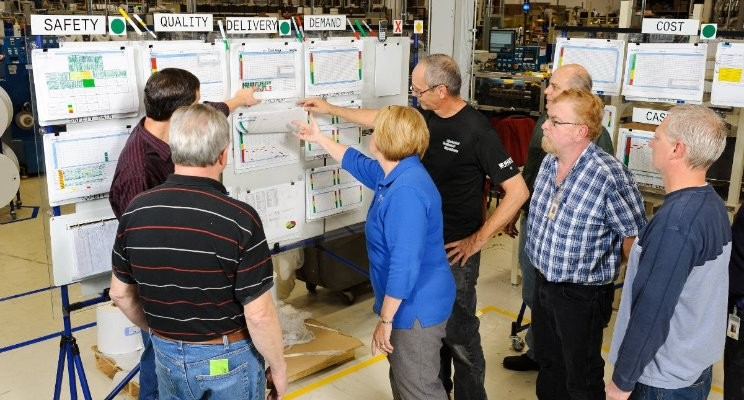
\includegraphics{01-imagenes/1520188654204.jpg}

}

\caption{Un grupo de trabajo en planta ante un panel de variables
indicadoras}

\end{figure*}

La estadística es la ciencia de aprender a partir de los datos. Implica
la recolección, análisis y presentación de los datos, y su utilización
para tomar decisiones y resolver problemas.

Hay muchos aspectos del trabajo industrial que implican recoger datos,
trabajar con ellos y utilizarlos para resolver un problema; el uso de la
estadística es sólo una herramienta más, tan importante como cualquier
otra disciplina en el bagaje de conocimientos de un científico,
ingeniero o técnico industrial.

Los métodos estadísticos nos ayudan a describir y comprender la
\textbf{variabilidad}. Cuando hablamos de variabilidad queremos decir
que sucesivas observaciones de un mismo proceso o sistema no dan
exactamente los mismos resultados. Por ejemplo, el consumo de gasolina
de un coche no es siempre igual, sino que varía de manera considerable.
Esta variación depende de muchos factores, como la forma de conducir, el
tipo de carretera, la situación del propio vehículo (presión de
neumáticos, compresión del motor, \ldots), la marca de la gasolina, el
octanaje, o incluso las condiciones meteorológicas. Todos estos factores
son causas de \textbf{variabilidad} en el consumo de gasolina. La
estadística nos permite analizar estos \textbf{factores} y determinar
cuáles son los más importantes o tienen mayor impacto en el consumo; una
vez conocidos, podemos actuar sobre ellos.

\begin{tcolorbox}[enhanced jigsaw, colback=white, opacitybacktitle=0.6, leftrule=.75mm, opacityback=0, coltitle=black, colframe=quarto-callout-important-color-frame, colbacktitle=quarto-callout-important-color!10!white, bottomrule=.15mm, title=\textcolor{quarto-callout-important-color}{\faExclamation}\hspace{0.5em}{Importante}, bottomtitle=1mm, toptitle=1mm, breakable, left=2mm, arc=.35mm, titlerule=0mm, rightrule=.15mm, toprule=.15mm]

El objetivo más importante de la mejora industrial es la
\textbf{reducción de la variabilidad}.

\end{tcolorbox}

En este libro aprenderemos a utilizar herramientas diversas, tanto
estadísticas como de la ciencia de datos, para realizar nuestro
análisis. Para aprender de los datos necesitamos más que los simples
números; para interpretarlos necesitaremos siempre el conocimiento del
proceso industrial que estamos analizando.En un análisis de la
producción de un producto lácteo, por ejemplo, los números significan
poco sin un conocimiento del proceso; los valores de pH, temperatura o
concentración de lactosa influyen en el resultado del proceso de forma
diferente. Los datos son números dentro de un contexto, y necesitamos
conocer este contexto para dar sentido a los números.

\begin{marginfigure}

{\centering 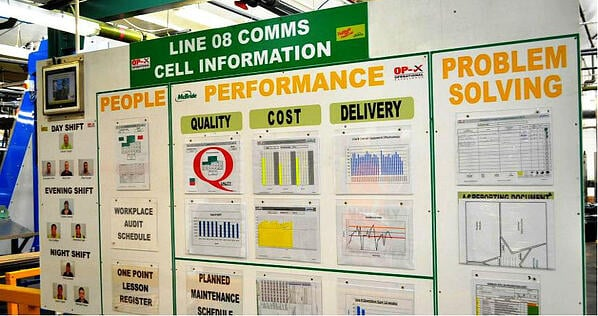
\includegraphics{01-imagenes/Lean-Visual-Management-Boards-in-Factories-Keep-It-Simple.jpg}

}

\end{marginfigure}

\hypertarget{pensamiento-estaduxedstico-y-pensamiento-cruxedtico-critical-thinking}{%
\section{\texorpdfstring{Pensamiento estadístico y pensamiento crítico
(\emph{Critical
Thinking})}{Pensamiento estadístico y pensamiento crítico (Critical Thinking)}}\label{pensamiento-estaduxedstico-y-pensamiento-cruxedtico-critical-thinking}}

Los ingenieros y técnicos resuelven problemas de interés para la empresa
y la sociedad mediante la aplicación de los principios del método
científico, siguiendo estos pasos:
{\marginnote{\begin{footnotesize}Razonamiento
estadístico\end{footnotesize}}}

\begin{enumerate}
\def\labelenumi{\arabic{enumi}.}
\tightlist
\item
  Preparar una descripción clara y concisa del problema
\item
  Identificar, al menos de forma tentativa, los principales factores que
  afectan al problema, o que podrían tener un papel en su resolución
\item
  Proponer un modelo para el problema, usando conocimiento científico o
  tecnológico del proceso en estudio, dejando constancia de las
  limitaciones del modelo propuesto.
\item
  Realizar experimentos apropiados y recolectar datos para probar o
  validar el modelo tentativo o las conclusiones previas obtenidas en
  los pasos 2 y 3
\item
  Refinar el modelo sobre la base de los datos observados
\item
  Manipular el modelo para desarrollar una solución al problema
\item
  Realizar un experimento adecuado para confirmar que la solución
  propuesta es efectiva y eficiente.
\item
  Sacar las conclusiones oportunas o hacer recomendaciones basándose en
  la solución encontrada.
\end{enumerate}

The definition of ``critical thinking'' used for construction of the
Halpern Critical Thinking Assessment characterizes critical thinking as
those cognitive skills or strategies that increase the probability of a
desirable outcome. They are purposeful, reasoned, and goal directed.
Critical thinking is the kind of thinking involved in solving problems,
formulating inferences, calculating likelihoods, and making decisions.
Critical thinkers use these skills appropriately, without prompting, and
usually with conscious intent, in a variety of settings. That is, they
are predisposed to think critically. When we think critically, we are
evaluating the outcomes of our thought processes-\/-how good a decision
is or how well a problem is solved. Critical thinking also involves
evaluating the thinking process-\/-the reasoning that went into the
conclusion we've arrived at or the kinds of factors considered in making
a decision. Therefore, critical thinking has to be regarded as a
hierarchical multidimen-sional construct comprising the facets verbal
reasoning, argument analysis skills, skills in thinking as hypothesis
testing, using likelihood and uncertainty, and decision making/problem
solving skills (Halpern, 1994; 1998; 2003). (APA PsycTests Database
Record (c) 2019 APA, all rights reserved)

\href{https://psycnet.apa.org/doiLanding?doi=10.1037\%2Ft10940-000}{HCTA
Halpern Critical Thinking Assessment (apa.org)}

\href{https://www.ed.ac.uk/institute-academic-development/study-hub/learning-resources/critical}{Critical
Thinking University of Edinbugh}

\hypertarget{what-is-critical-thinking}{%
\subsection{What is critical
thinking?}\label{what-is-critical-thinking}}

\begin{quote}
Critical thinking is the art of making clear, reasoned judgements based
on interpreting, understanding, applying and synthesising evidence
gathered from observation, reading and experimentation.

Burns, T., \& Sinfield, S. (2016)~Essential Study Skills: The Complete
Guide to Success at University (4th ed.) London: SAGE, p94.
\end{quote}

Being critical does not just mean finding fault.~ It means assessing
evidence from a variety of sources and making reasoned conclusions.~ As
a result of your analysis you may decide that a particular piece of
evidence is not robust, or that you disagree with the conclusion, but
you should be able to state why you have come to this view and
incorporate this into a bigger picture of the literature.

Being critical goes beyond describing what you have heard in lectures or
what you have read.~ It involves synthesising, analysing and evaluating
what you have learned to develop your own argument or position.

Critical thinking is important in all subjects and disciplines -- in
science and engineering, as well as the arts and humanities.~ The types
of evidence used to develop arguments may be very different but the
processes and techniques are similar.~ Critical thinking is required for
both undergraduate and postgraduate levels of study.

\hypertarget{what-where-when-who-why-how}{%
\subsection{What, where, when, who, why,
how?}\label{what-where-when-who-why-how}}

Purposeful reading can help with critical thinking because it encourages
you to read actively rather than passively.~ When you read, ask yourself
questions about what you are reading and make notes to record your
views.~ Ask questions like:

\begin{itemize}
\item
  What is the main point of this paper/ article/ paragraph/ report/
  blog?
\item
  Who wrote it?
\item
  Why was it written?
\item
  When was it written?
\item
  Has the context changed since it was written?
\item
  Is the evidence presented robust?
\item
  How did the authors come to their conclusions?
\item
  Do you agree with the conclusions?
\item
  What does this add to our knowledge?
\item
  Why is it useful?
\end{itemize}

\hypertarget{developing-an-argument}{%
\subsection{Developing an argument}\label{developing-an-argument}}

Being a university student is about learning how to think, not what to
think.~ Critical thinking shapes your own values and attitudes through a
process of deliberating, debating and persuasion.~~ Through developing
your critical thinking you can move on from simply disagreeing to
constructively assessing alternatives by building on doubts.

There are several key stages involved in developing your ideas and
constructing an argument.~ You might like to use a form to help you
think about the features of critical thinking and to break down the
stages of developing your argument.

\url{https://elpais.com/economia/estar-donde-estes/2021-03-24/como-aplicar-el-pensamiento-critico-en-tu-trabajo.html}

\href{https://www.ed.ac.uk/institute-academic-development/study-hub/learning-resources/statistical-and-numerical-data}{Statistical
and numerical data}

\hypertarget{algunas-definiciones-importantes}{%
\section{Algunas definiciones
importantes}\label{algunas-definiciones-importantes}}

\hypertarget{poblaciuxf3n-y-muestra}{%
\subsection{Población y muestra}\label{poblaciuxf3n-y-muestra}}

Una \textbf{población} es un conjunto de de personas, cosas o, en
general, objetos en estudio. A veces, una población es demasiado grande
para que podamos abarcarla completa; para poder estudiarla, obtenemos
una \textbf{muestra}, que consiste en un subconjunto de la población que
hemos seleccionado para su estudio. El proceso de obtener una muestra se
llama \textbf{muestreo}, y se realiza de acuerdo con normas y
procedimientos específicos.

En muchas ocasiones, cuando se recogen los datos como resultado de una
experimentación, definimos la población como \emph{todos los resultados
que podríamos haber obtenido}. Llamamos a este conjunto de posibles
resultados una \textbf{población conceptual}. Por ejemplo, cuando
medimos el \(pH\) de varias muestras de leche, la población es el
conjunto de todos los resultados posibles que podríamos haber tenido.
Muchos problemas de ingeniería y tecnología se refieren a poblaciones
conceptuales.

\begin{tcolorbox}[enhanced jigsaw, colback=white, opacitybacktitle=0.6, leftrule=.75mm, opacityback=0, coltitle=black, colframe=quarto-callout-important-color-frame, colbacktitle=quarto-callout-important-color!10!white, bottomrule=.15mm, title=\textcolor{quarto-callout-important-color}{\faExclamation}\hspace{0.5em}{Recuerda}, bottomtitle=1mm, toptitle=1mm, breakable, left=2mm, arc=.35mm, titlerule=0mm, rightrule=.15mm, toprule=.15mm]

En la mayoría de las ocasiones, nuestros datos provienen de una
\textbf{muestra} obtenida de una \textbf{población},

\end{tcolorbox}

Cuando tomamos una muestra, debemos estar seguros de que contiene las
propiedades que queremos estudiar en la población. En ese caso, decimos
que la muestra es \textbf{representativa}: los individuos de la muestra
son representativos de la población. Para que la muestra sea
representativa, debe ser obtenida mediante un \textbf{muestreo
aleatorio}. Una \textbf{muestra aleatoria simple} de tamaño \(n\)
consiste en \(n\) individuos de una población, elegidos de forma que
cada conjunto posible de \(n\) individuos tiene la misma
\textbf{probabilidad} de ser elegido

\begin{tcolorbox}[enhanced jigsaw, colback=white, opacitybacktitle=0.6, leftrule=.75mm, opacityback=0, coltitle=black, colframe=quarto-callout-important-color-frame, colbacktitle=quarto-callout-important-color!10!white, bottomrule=.15mm, title=\textcolor{quarto-callout-important-color}{\faExclamation}\hspace{0.5em}{¿Qué es la probabilidad?}, bottomtitle=1mm, toptitle=1mm, breakable, left=2mm, arc=.35mm, titlerule=0mm, rightrule=.15mm, toprule=.15mm]

Introduciremos el concepto de probabilidad con detalle en el capítulo 4

\end{tcolorbox}

\hypertarget{paruxe1metro-y-estaduxedstico}{%
\subsection{Parámetro y
estadístico}\label{paruxe1metro-y-estaduxedstico}}

Llamamos \textbf{estadístico} a un número que representa una propiedad o
característica de la muestra. Un \textbf{parámetro} es una
característica de la población, que podemos estimar a partir de la
muestra mediante la obtención de un \textbf{estadístico muestral}.

\hypertarget{variables-y-casos}{%
\subsection{Variables y casos}\label{variables-y-casos}}

A los objetos descritos en un conjunto de datos los llamamos
\textbf{casos}, de forma genérica. A veces, estos casos pueden
corresponder a personas; en ese caso podemos llamarlos
\textbf{individuos}. Cuando los objetos que estudiamos no son personas,
como es lo habitual en el entorno industrial, utilizamos la nomenclatura
genérica.

Un \textbf{atributo} es una característica que define una propiedad de
un objeto, persona o cosa. Por ejemplo, edad, peso, altura, sexo, color
de ojos, son atributos de una persona. Llamamos \textbf{variable} a una
característica cualquiera de un individuo que puede ser medida. Una
variable puede tomar diferentes valores en diferentes individuos o
casos.

Según estas definiciones que acabamos de ver, una muestra está formada
por un conjunto de casos, y cada caso contiene un determinado número de
variables, que contienen los valores que hemos analizado o medido.

\begin{tcolorbox}[enhanced jigsaw, colback=white, opacitybacktitle=0.6, leftrule=.75mm, opacityback=0, coltitle=black, colframe=quarto-callout-note-color-frame, colbacktitle=quarto-callout-note-color!10!white, bottomrule=.15mm, title={Ejemplo 1: Muestreando una cámara de maduración de queso}, bottomtitle=1mm, toptitle=1mm, breakable, left=2mm, arc=.35mm, titlerule=0mm, rightrule=.15mm, toprule=.15mm]

Imagínate que tienes que analizar el extracto seco de una producción de
queso que está en fase de maduración en una cámara. Como la cámara está
muy llena, es difícil acceder al interior, y decides coger tu muestra de
los quesos que están más a tu alcance, justo al lado de la puerta y a la
altura de la vista.¿Crees que es una buena idea? ¿Podrías definir la
población en este caso?.

\end{tcolorbox}

\begin{tcolorbox}[enhanced jigsaw, colback=white, opacitybacktitle=0.6, leftrule=.75mm, opacityback=0, coltitle=black, colframe=quarto-callout-tip-color-frame, colbacktitle=quarto-callout-tip-color!10!white, bottomrule=.15mm, title={Respuesta al ejemplo 1: Muestreando una cámara de maduración de queso}, bottomtitle=1mm, toptitle=1mm, breakable, left=2mm, arc=.35mm, titlerule=0mm, rightrule=.15mm, toprule=.15mm]

No es una buena idea porque no tenemos garantía de que las condiciones
de humedad,temperatura y circulación de aire sean las mismas en toda la
cámara. Para asegurar que nuestra muestra es representativa, debemos
tomar una \textbf{muestra aleatoria} de la población, que en este caso
es el total de quesos en la cámara.

\end{tcolorbox}

\hypertarget{tipos-de-variables}{%
\subsection{Tipos de variables}\label{tipos-de-variables}}

Algunas variables, como el color, sirven para clasificar los individuos
en categorías. Otras, como la altura o el peso de un individuo, pueden
tomar valores numéricos con los que podemos hacer cálculos. Por ejemplo,
podemos sumar la altura de varias personas, pero no tiene sentido
\emph{sumar} los colores del arco-iris (aunque sí podemos
\emph{contarlos}, y hacer cálculos con estos recuentos). También podemos
\emph{categorizar} variables continuas: podemos clasificar nuestro grupo
de personas en \emph{altas} o \emph{bajas}, y podemos contar cuántas
personas entran en cada categoría.

\begin{longtable}[]{@{}
  >{\raggedright\arraybackslash}p{(\columnwidth - 6\tabcolsep) * \real{0.2568}}
  >{\raggedright\arraybackslash}p{(\columnwidth - 6\tabcolsep) * \real{0.2432}}
  >{\raggedright\arraybackslash}p{(\columnwidth - 6\tabcolsep) * \real{0.2568}}
  >{\raggedright\arraybackslash}p{(\columnwidth - 6\tabcolsep) * \real{0.2432}}@{}}
\toprule\noalign{}
\begin{minipage}[b]{\linewidth}\raggedright
Variables cualitativas o categóricas
\end{minipage} & \begin{minipage}[b]{\linewidth}\raggedright
\end{minipage} & \begin{minipage}[b]{\linewidth}\raggedright
Variables cuantitativas o métricas
\end{minipage} & \begin{minipage}[b]{\linewidth}\raggedright
\end{minipage} \\
\midrule\noalign{}
\endhead
\bottomrule\noalign{}
\endlastfoot
\textbf{Nominales} & \textbf{Ordinales} & \textbf{Discretas} &
\textbf{Continuas} \\
Valores en categorías arbitrarias & Valores en categorías ordenadas &
Valores enteros en escala numérica & Valores continuos en escala
numérica \\
(sin unidades) & (sin unidades) & Unidades contadas & Unidades
medidas \\
\end{longtable}

\begin{table}[]
\centering
\begin{tabular}{@{}cccc@{}}
\toprule
\multicolumn{2}{c}{\textbf{\begin{tabular}[c]{@{}c@{}}Variables\\ cualitativas\\ o categóricas\end{tabular}}} &
  \multicolumn{2}{c}{\textbf{\begin{tabular}[c]{@{}c@{}}Variables \\ cuantitativas\\ o métricas\end{tabular}}} \\ 
\cmidrule(lr){1-2} \cmidrule(lr){3-4}
\textbf{Nominales} &
  \textbf{Ordinales} &
  \textbf{Discretas} &
  \textbf{Continuas} \\ 
\cmidrule(lr){1-2} \cmidrule(lr){3-4}
\begin{tabular}[c]{@{}c@{}}Valores\\ en categorías \\ arbitrarias\end{tabular} &
  \begin{tabular}[c]{@{}c@{}}Valores \\ en categorías\\ ordenadas\end{tabular} &
  \begin{tabular}[c]{@{}c@{}}Valores enteros\\ en una escala \\ numérica\end{tabular} &
  \begin{tabular}[c]{@{}c@{}}Valores continuos\\ en una escala \\ numérica\end{tabular} \\
(sin unidades) &
  (sin unidades) &
  \begin{tabular}[c]{@{}c@{}}Unidades\\ contadas\end{tabular} &
  \begin{tabular}[c]{@{}c@{}}Unidades\\ medidas\end{tabular} \\ \bottomrule
\end{tabular}
\end{table}

Una \textbf{variable categórica} coloca a un individuo en uno o más
grupos o categorías

Una \textbf{variable métrica} toma valores numéricos con los que tiene
sentido realizar cálculos aritméticos como sumar, restar, etc.

Las variables categóricas se conocen también como \textbf{variables
cualitativas} porque indican \emph{cualidades}.

Las variables métricas se conocen también como \textbf{variables
cuantitativas} porque indican \emph{cantidades}.

\begin{tcolorbox}[enhanced jigsaw, colback=white, opacitybacktitle=0.6, leftrule=.75mm, opacityback=0, coltitle=black, colframe=quarto-callout-warning-color-frame, colbacktitle=quarto-callout-warning-color!10!white, bottomrule=.15mm, title=\textcolor{quarto-callout-warning-color}{\faExclamationTriangle}\hspace{0.5em}{Comentario: ¿Cualitativo quiere decir ``que tiene calidad''?}, bottomtitle=1mm, toptitle=1mm, breakable, left=2mm, arc=.35mm, titlerule=0mm, rightrule=.15mm, toprule=.15mm]

A veces se utiliza la palabra \textbf{cualitativo} de forma incorrecta
para indicar \textbf{calidad}, por ejemplo cuando alguien dice: ``Este
envase es muy \textbf{cualitativo}''. Deberíamos decir ``Este envase
tiene gran calidad''. \textbf{Cualitativo} no se deriva de
\textbf{calidad}, sino de \textbf{cualidad}.

\end{tcolorbox}

\hypertarget{ejemplos-de-variables}{%
\subsection{Ejemplos de variables}\label{ejemplos-de-variables}}

\begin{tcolorbox}[enhanced jigsaw, colback=white, opacitybacktitle=0.6, leftrule=.75mm, opacityback=0, coltitle=black, colframe=quarto-callout-note-color-frame, colbacktitle=quarto-callout-note-color!10!white, bottomrule=.15mm, title={Para resolver}, bottomtitle=1mm, toptitle=1mm, breakable, left=2mm, arc=.35mm, titlerule=0mm, rightrule=.15mm, toprule=.15mm]

\textbf{Ejemplo 1}. Tiramos un dado al aire. Describe a qué corresponde
la variable y el caso.

\textbf{Ejemplo 2}. Durante un proceso de envasado de un producto que
dura una hora, controlamos el peso de cada envase cada minuto. Describe
la variable y el caso. ¿Puede haber más de una variable?

\end{tcolorbox}

\begin{tcolorbox}[enhanced jigsaw, colback=white, opacitybacktitle=0.6, leftrule=.75mm, opacityback=0, coltitle=black, colframe=quarto-callout-tip-color-frame, colbacktitle=quarto-callout-tip-color!10!white, bottomrule=.15mm, title={Respuestas: Para resolver}, bottomtitle=1mm, toptitle=1mm, breakable, left=2mm, arc=.35mm, titlerule=0mm, rightrule=.15mm, toprule=.15mm]

\textbf{Ejemplo 1}: La \textbf{variable} es el resultado que obtenemos
cada vez; podríamos denominarla, por ejemplo, \(resultado\_obtenido\).
Colocaríamos este nombre en el encabezado de una columna en una hoja de
cálculo. Cada tirada que hacemos es un \textbf{caso}; iríamos colocando
el resultado que obtenemos cada vez en una nueva fila de nuestra hoja de
cálculo.

\textbf{Ejemplo 2}. En este caso, la \textbf{variable} es el
\(peso\_obtenido\), y cada pesada constituye un \textbf{caso}. Si
registrásemos, además, la hora y el minuto en el que que hemos hecho
cada control de peso, podríamos definir una nueva variable, que
podríamos llamar \(hora\), y que colocaríamos en una columna al lado del
\(peso\_obtenido\). Incluso podríamos definir otra variable adicional,
el \(numero\_de\_pesada\), que sería un número secuencial empezando en
\(1\) y que se incrementaría en cada pesada, de forma que al final esta
variable nos daría el número de pesadas realizadas, y nos indicaría
además el orden en el que las hemos realizado. Puesto que hemos
realizado una pesada cada minuto, tendríamos tres variables y 61 líneas
(un encabezado y 60 líneas correspondientes una a cada minuto)

\end{tcolorbox}

\bookmarksetup{startatroot}

\hypertarget{herramientas-para-el-anuxe1lisis-de-los-datos-industriales}{%
\chapter{Herramientas para el análisis de los datos
industriales}\label{herramientas-para-el-anuxe1lisis-de-los-datos-industriales}}

\hypertarget{las-hojas-de-cuxe1lculo.}{%
\section{Las hojas de cálculo.}\label{las-hojas-de-cuxe1lculo.}}

La hoja de cálculo es una herramienta omnipresente hoy día en todos los
ámbitos de trabajo y educativos. Desde la aparición de
\href{https://es.wikipedia.org/wiki/VisiCalc}{Visicalc}, en 1978, la
hoja de cálculo ha contribuido a la gestión de miles de empresas, se ha
utilizado de manera general en análisis de datos y sus gráficos se han
utilizado y se utilizan en publicaciones e informes de todas clases. En
la década de los años 80 del pasado siglo, la hoja de cálculo
\href{https://es.wikipedia.org/wiki/Lotus_1-2-3}{Lotus 1-2-3} fue la
aplicación más utilizada en los ordenadores IBM-PC y compatibles, y
consiguió facturaciones millonarias para la empresa matriz. Lotus 1-2-3
dominó el mercado hasta la aparición de Microsoft Windows a finales de
los años 80; el nuevo sistema operativo favoreció la implantación de
Excel, que desde entonces se convirtió en la hoja de cálculo dominante.

\begin{figure}

\begin{minipage}[t]{0.50\linewidth}

{\centering 

\raisebox{-\height}{

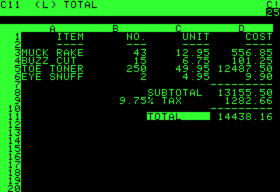
\includegraphics{01-imagenes/280px-Visicalc.png}

}

\caption{Visicalc, primera hoja de cálculo para el ordenador \emph{Apple
II} (1979)}

}

\end{minipage}%
%
\begin{minipage}[t]{0.50\linewidth}

{\centering 

\raisebox{-\height}{

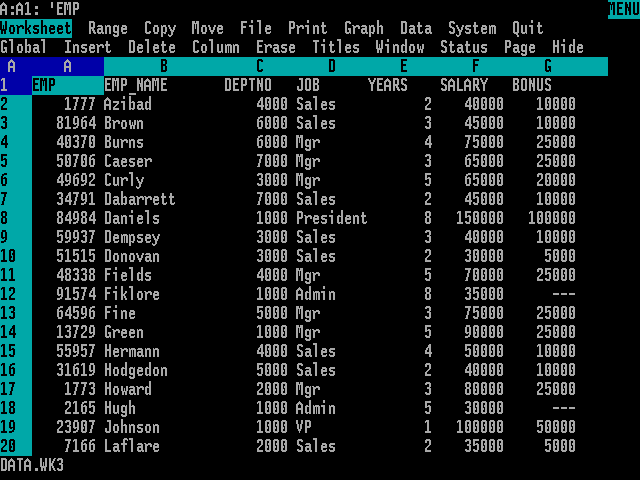
\includegraphics{01-imagenes/Lotus-123-3.0-MSDOS.png}

}

\caption{Hoja de cálculo Lotus 1-2-3 para MS-DOS (1983)}

}

\end{minipage}%
\newline
\begin{minipage}[t]{\linewidth}

{\centering 

\raisebox{-\height}{

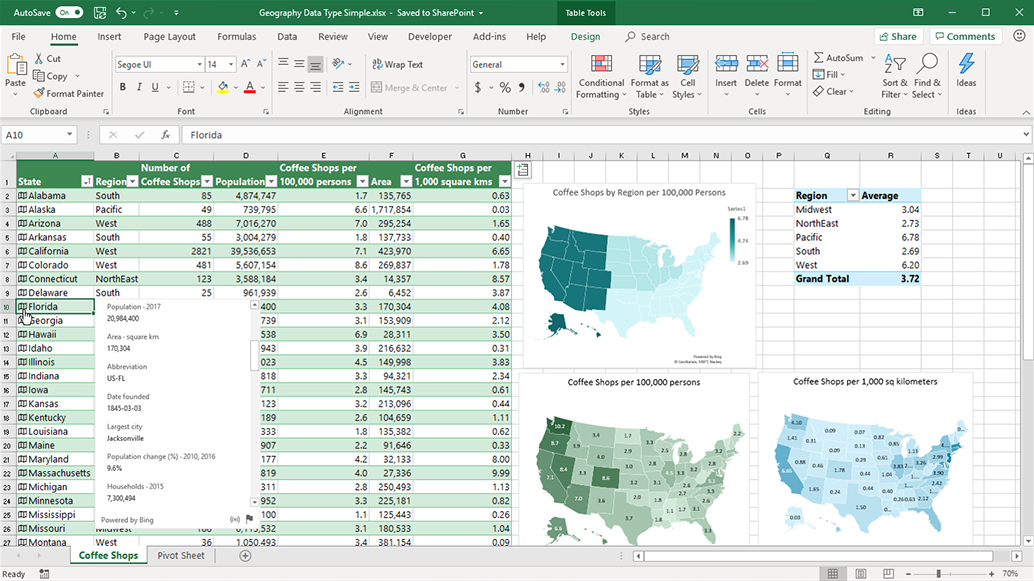
\includegraphics{01-imagenes/excel.png}

}

\caption{Microsoft Excel (2023)}

}

\end{minipage}%

\end{figure}

\hypertarget{el-software-estaduxedstico-r}{%
\section{El software estadístico R}\label{el-software-estaduxedstico-r}}

\hypertarget{almacenar-datos-en-una-hoja-de-cuxe1lculo}{%
\section{Almacenar datos en una hoja de
cálculo}\label{almacenar-datos-en-una-hoja-de-cuxe1lculo}}

Las \textbf{hojas de cálculo} son muy útiles para recoger la información
de un conjunto de observaciones. De la misma manera que la gramática
permite ordenar y estructurar un escrito de acuerdo a reglas comunes,
veremos que hay reglas para que el almacenamiento de los datos sea lo
más homogéneo posible y se reduzcan los errores al mínimo.

En este libro trataremos exclusivamente de lo que llamaremos
\textbf{datos rectangulares}: grupos de valores que están asociados a
una o más variables, y a varias observaciones. Hay muchos más datos que
no se ajustan a este paradigma: imágenes, sonidos, archivos documentales
de texto. Pero la forma más común de almacenar datos industriales es la
de las tablas rectangulares; vamos a aprender cómo organizarlas
correctamente.

\hypertarget{preparaciuxf3n-de-los-datos}{%
\subsection{Preparación de los
datos}\label{preparaciuxf3n-de-los-datos}}

Los datos se pueden recoger y guardar de múltiples formas. Cuando nos
incorporamos a un equipo de trabajo existente, lo más seguro es que el
equipo disponga ya de un sistema de archivo de los datos, de acuerdo con
sus prácticas habituales.

Cuando la recogida de datos se hace de forma manual en papel, es
necesario registrar en el ordenador los datos recogidos. Lo más
frecuente es que este registro se haga en hojas de cálculo, como
\href{https://www.microsoft.com/es-es/microsoft-365/excel}{Microsoft
Excel} o \href{https://www.google.es/intl/es/sheets/about/}{Google
Sheets}. En algunos casos, el almacenamiento se hace sobre bases de
datos, genéricas o desarrolladas a medida.

Actualmente, la tendencia es recoger los datos o bien de forma
automática, o bien de forma manual sobre sistemas informatizados
(pantallas), lo que permite eliminar el papel y disponer directamente de
los datos en un formato digitalizado.

Los equipos y líneas de producción diseñados actualmente (IoT) se
interconectan con los sistemas de información y almacenan en tiempo real
todos los datos necesarios, lo que libera al operario de la pesada tarea
de reintroducirlos manualmente, a la vez que reduce los errores debidos
a la imputación incorrecta.

En todos los casos, es imprescindible asegurar que los sistemas de
información pueden exportar a ficheros de texto tipo \emph{fichero
plano} o tipo CSV, de forma que podamos importarlos tanto a Excel como a
R, como veremos más adelante. Estos sistemas de exportación de datos
deben diseñarse de forma flexible y abierta, para que tanto la captura
como la exportación puedan modificarse y adaptar la recogida de la
información a las necesidades de cada momento.

\hypertarget{diseuxf1o-de-la-captura-de-informaciuxf3n}{%
\subsection{Diseño de la captura de
información}\label{diseuxf1o-de-la-captura-de-informaciuxf3n}}

A veces el diseño de la captura de datos sigue aproximadamente el modelo
manual en papel. Se introducen los datos en la hoja de cálculo y una vez
completados, se imprime el documento para su archivo.

El error más común que cometemos es tratar la hoja de cálculo como un
bloc de notas, es decir, hacer anotaciones de forma libre, colocar los
datos y el resultado de los análisis al lado y en cualquier parte de la
hoja, y apoyarnos en el contexto para interpretar lo que hemos guardado.
Pero para que el ordenador sea capaz de analizar nuestros datos de
manera eficiente, debemos estructurarlos de tal forma que el programa
use la información tal como nosotros queremos.

Es común utilizar una hoja para guardar múltiples tablas de datos, tal
como vemos en la Figura~\ref{fig-excel_mess}. Esta estructura, sin
embargo, resulta enormemente confusa para su análisis, o lo imposibilita
completamente.

\begin{figure}

{\centering 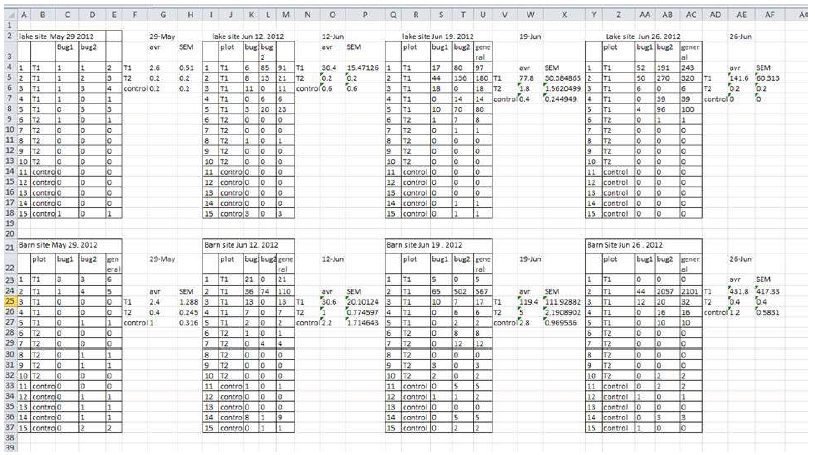
\includegraphics{01-imagenes/excel_mess.png}

}

\caption{\label{fig-excel_mess}Hoja Excel desordenada: ¡No hagas esto!}

\end{figure}

En otros casos, los datos se guardan en hojas de cálculo que se componen
de diferentes pestañas para cada semana, cada mes o cada año, como vemos
en la Figura~\ref{fig-2021-09-1_excel_1}. Sin embargo, esta forma de
almacenar los datos tampoco es la óptima para su análisis.

\begin{figure}

{\centering 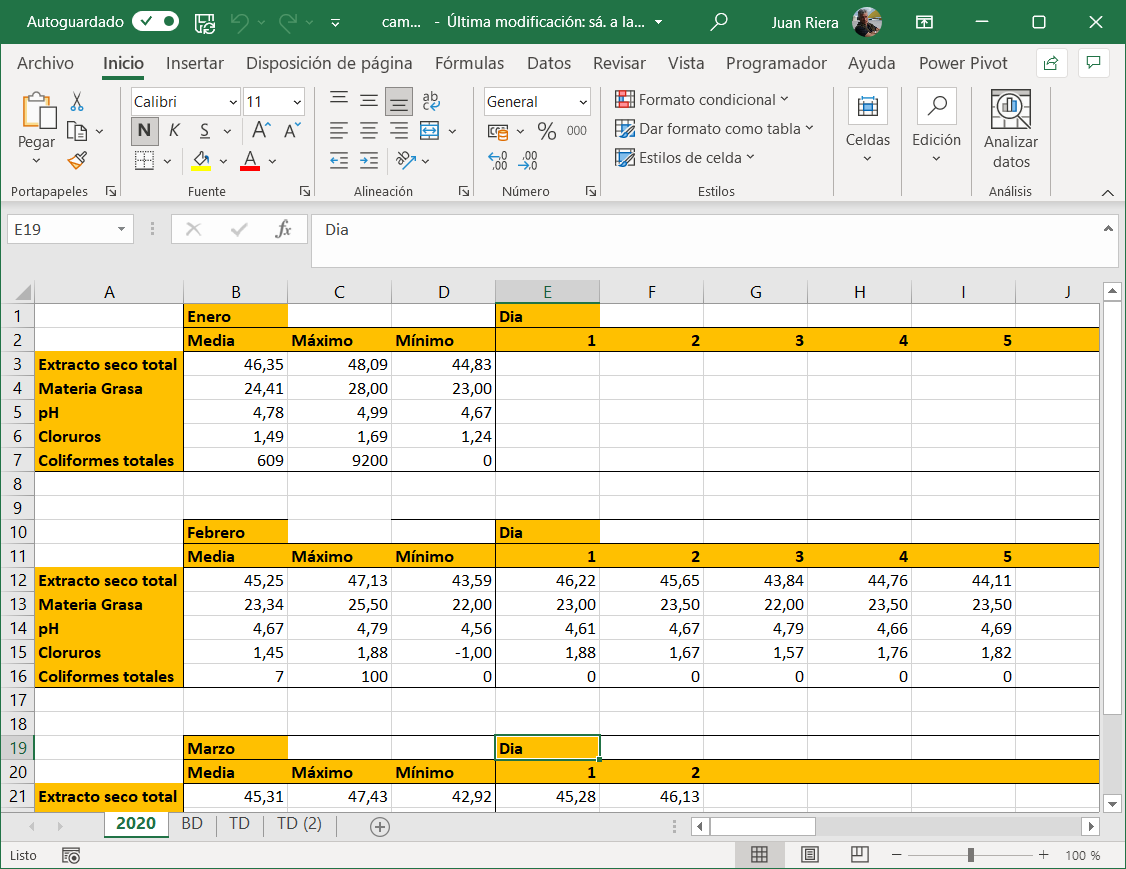
\includegraphics{01-imagenes/2021-09-1_excel_1.png}

}

\caption{\label{fig-2021-09-1_excel_1}Hoja Excel con una estructura no
ordenada}

\end{figure}

¿Y utilizar diferentes pestañas para cada tabla? En este caso, la
respuesta es sí y no. Si las diferentes tablas presentan situaciones
diferentes, o datos que no son coincidentes, podemos utilizar diferentes
pestañas. Pero si los datos están vinculados, por ejemplo, se
corresponden con medidas hechas en fechas diferentes (meses, años), la
respuesta adecuada es que las pestañas no son la forma correcta de
almacenarlos datos; la forma recomendad es añadir una variable que nos
permita diferenciar los datos por fecha; nuestro programa de análisis
nos permitirá \emph{filtrar} los datos según la fecha que deseemos, y
todos estarán en una única tabla, facilitando la coherencia del
conjunto.

Hay muchas formas de almacenar la información en una hoja de cálculo,
pero hay una forma que facilita la utilización de los datos tanto por la
hoja de cálculo como por otros programas de análisis, A esta forma de
almacenar las tablas de datos la llamamos \textbf{datos ordenados}
(\emph{tidy data})(Wickham 2014)

\hypertarget{los-datos-ordenados-tidy-data}{%
\section{\texorpdfstring{Los datos ordenados (\emph{tidy
data})}{Los datos ordenados (tidy data)}}\label{los-datos-ordenados-tidy-data}}

\begin{marginfigure}

{\centering 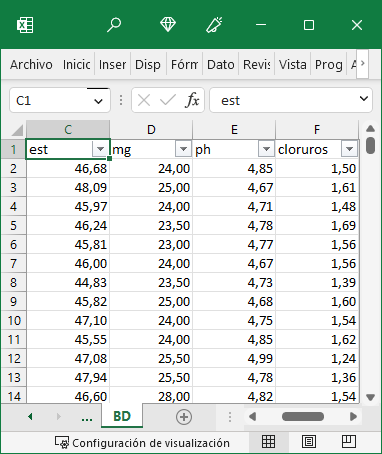
\includegraphics{01-imagenes/2023-01-20.png}

}

\caption{\label{fig-excel-camembert}Hoja Excel con estructura
rectangular de datos ordenados}

\end{marginfigure}

Las reglas principales al almacenar nuestros datos en una hoja de
cálculo es que columnas=variables, filas=observaciones, celdas=valores.
Estas tres reglas básicas son las que hacen que nuestro conjunto de
datos sea ordenado (Hadley Wickham 2017):

\begin{enumerate}
\def\labelenumi{\arabic{enumi}.}
\tightlist
\item
  Cada variable debe tener su propia columna.
\item
  Cada observación debe tener su propia fila.
\item
  Cada valor debe tener su propia celda o casilla .
\end{enumerate}

La Figura~\ref{fig-tidy1} muestra estas reglas de forma visual.

\begin{figure}

{\centering 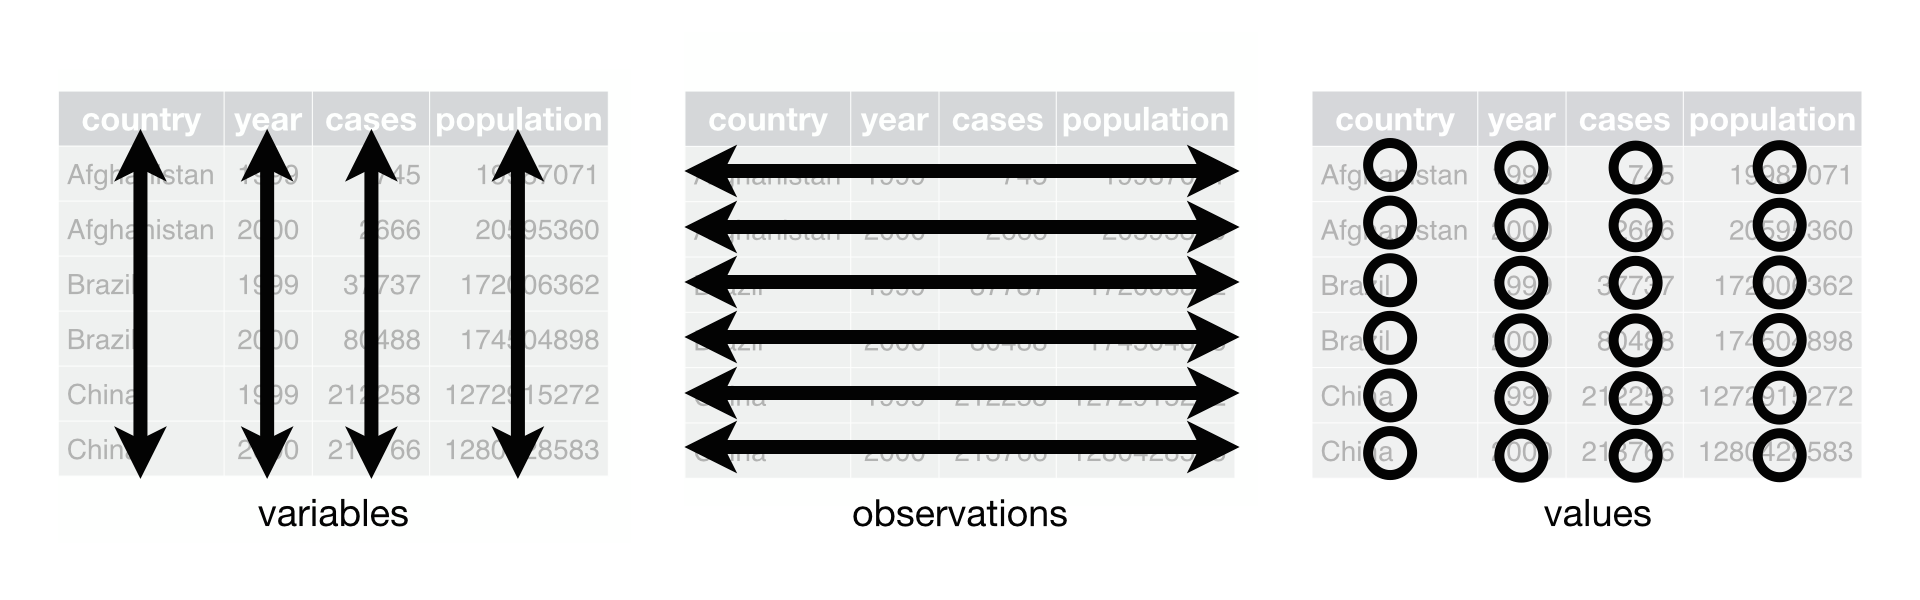
\includegraphics{01-imagenes/tidy-1.png}

}

\caption{\label{fig-tidy1}Sigue estas tres reglas para tener un conjunto
de datos ordenado: las variables están en columnas, las observaciones
están en filas, y los valores están en celdas. Fuente de la imagen:
{[}@wickham2017{]}}

\end{figure}

Estas tres reglas están interrelacionadas porque es imposible satisfacer
sólo dos de tres.

\hypertarget{los-nombres-de-las-variables}{%
\section{Los nombres de las
variables}\label{los-nombres-de-las-variables}}

Según hemos visto, existen diferentes tipos de variables,
\textbf{cualitativas} (\emph{categóricas}) y \textbf{cuantitativas}
(\emph{métricas}). Normalmente, los valores de las variables categóricas
se describen mediante textos del tipo ``color blanco'', ``hombre'',
``mujer'', ``alto'', ``bajo'', etc. Suelen corresponder con
características descriptivas, y por lo tanto, no puede hacerse cálculos
directamente con ellos, a menos que se hayan resumido, por ejemplo,
mediante un conteo. Las variables métricas consisten en valores
numéricos, que pueden ser \textbf{enteros} (\(1\);\(24\);\(350\)) o
\textbf{continuos} (\(1,456\);\(0,35\)) y que sí pueden utilizarse
directamente para hacer cálculos tales como sumas, etc.

Una \textbf{variable} está descrita siempre por \textbf{un nombre}, que
designa la variable, y \textbf{un valor o conjunto de valores}, que
corresponden a los casos. Este conjunto de valores, como acabamos de
ver, pueden ser textos o números.

{\marginnote{\begin{footnotesize}Existen también otros tipos de
variables que veremos más tarde, como variables lógicas o fechas, según
el tipo de dato que almacenemos en esa variable.\end{footnotesize}}}

Ejemplos de valores de texto: ``Carlos'', ``fruta'', ``Lluvia fuerte'',
``muy ácido'', ``sabor a fresa''

Ejemplos de valores numéricos: \(1\); \(7\); \(10,65\)

Siempre que sea posible, utilizaremos el nombre del atributo o
característica que estamos midiendo o analizando, o su abreviatura, para
designar una variable; por ejemplo, si estamos recogiendo la altura de
una serie de personas, llamaremos \texttt{altura} a la variable; si
estamos recogiendo el peso, usaremos el nombre \texttt{peso}, etc.

En una hoja de cálculo, colocaremos el nombre de la variable en la
primera fila, e iremos añadiendo los valores debajo, un valor por línea.

A veces, asignar un nombre a una variable no es todo lo fácil que podría
parecer a simple vista. Por ejemplo, ¿qué nombre daríamos a una variable
que va a recoger los valores de \(pH\) de la leche en una cuba de queso
en el momento de añadir el cuajo? Está claro que \(pH\) no es
suficiente, porque en el proceso hay varias medidas de \(pH\) y sería
bueno que pudiésemos diferenciarlas con facilidad. En un caso como éste,
es probable que necesitemos utilizar varias palabras o abreviaturas que
describan mejor el nombre de la variable.

\begin{marginfigure}

{\centering 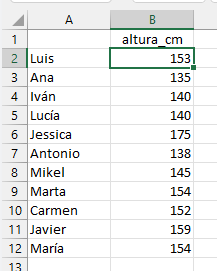
\includegraphics{01-imagenes/aula1.png}

}

\end{marginfigure}

Para la construcción correcta de estos nombres, se han establecido un
conjunto de normas, con el objetivo de evitar errores y facilitar el
intercambio de los datos entre diferentes programas de análisis.

\hypertarget{reglas-para-los-nombres-de-las-variables}{%
\subsection{Reglas para los nombres de las
variables}\label{reglas-para-los-nombres-de-las-variables}}

Las hojas de cálculo admiten que introduzcamos cualquier texto en una
celda; no hay prácticamente ninguna limitación a los nombres que podemos
usar para nuestras variables. Excel utilizará los nombres con cualquier
carácter sin inconvenientes.

Sin embargo, otros programas informáticos, entre ellos R, son mucho más
restrictivos. Por esta razón, estableceremos una serie de reglas para
construir los nombres de variables, que aplicaremos a nuestras tablas de
Excel, y que nos permitirán intercambiarlas con otros programas, como R,
con toda seguridad.

\begin{enumerate}
\def\labelenumi{\arabic{enumi}.}
\tightlist
\item
  Un nombre válido consiste en una combinación de letras, números y
  signo de subrayado (\(\_\))
\item
  Un nombre de variable no puede empezar por un número, un punto o un
  signo de subrayado (\(\_\)); debe empezar siempre por una letra.
\item
  Los nombres de variables irán siempre en minúsculas. Según esta regla,
  \(Peso\) no es un nombre válido, pero \(peso\) si lo es.
\end{enumerate}

{\marginnote{\begin{footnotesize}En R, las mayúsculas son significativas
es decir, en R, \(peso\) y \(Peso\) son nombres diferentes. Por esta
razón, aunque el uso de mayúsculas está permitido, nosotros adoptaremos
las minúsculas de forma general)\end{footnotesize}}}

\begin{enumerate}
\def\labelenumi{\arabic{enumi}.}
\setcounter{enumi}{3}
\item
  No utilizaremos espacios en blanco, acentos ni caracteres especiales
  como \(\tilde{n}\), \(\%\), guiones o paréntesis.
\item
  Hay veces en que nos interesa unir varias palabras para construir un
  nombre de variable. Se utilizan diferentes formas de unir palabras,
  por ejemplo:

  \begin{itemize}
  \item
    un punto, como en \(peso.en.cm\),
  \item
    lo que se ha llamado \emph{escritura de camello} (\emph{camelCase}),
    que se llama así por el uso de mayúsculas y minúsculas mezcladas
    (\(PesoEnCm\))
  \item
    el signo de subrayado \(\_\), como en \(peso\_en\_cm\)
  \end{itemize}

  Algunas de estas opciones son utilizadas en distintas comunidades de
  usuarios, por ejemplo la opción 1 es utilizada en la guía de estilo de
  Google, y la opción 2 es muy utilizada por los programadores del
  entorno de los lenguajes de Microsoft. Nosotros utilizaremos el signo
  de subrayado (\(\_\)), que es la forma más usada en el entorno de
  programación de R.
\item
  Siempre se separarán las palabras mediante el signo de subrayado (\_)
  para facilitar la lectura. Así, aunque \(temperatura1\) es un nombre
  válido, preferiremos \(temp\_1\); es más corto y de lectura más clara.
  Igualmente, preferiremos \(peso\_empaquetado\) a \(pesoempaquetado\)
\item
  Mantendremos los nombres razonablemente cortos para facilitar la
  lectura. Aunque podemos hacer los nombres todo lo largos que queramos,
  es más cómodo utilizar nombres cortos. Por ejemplo, podríamos utilizar
  \(temperatura\_de\_la\_leche\_al\_cuajar\), pero preferiremos
  abreviarlo como \(temp\_cuajo\).
\end{enumerate}

Nombres no válidos:

\begin{itemize}
\tightlist
\item
  \(peso\ en\ gramos\) (contiene espacios)
\item
  \(pH\_de\_la\_leche\_en\_Recepci\acute{o}n\) (demasiado largo, tiene
  un acento, tiene mayúsculas)
\item
  \(extracto\_seco\_total\_a\_la\_salida\_de\_la\_salmuera\) (demasiado
  largo)
\end{itemize}

Alternativas válidas:

\begin{itemize}
\tightlist
\item
  \(peso\_g\)
\item
  \(pH\_leche\_rec\) (en este caso, de manera excepcional, podemos
  mantener el uso de la mayúscula por corrección formal)
\item
  \(est\_salida\_sal\)
\end{itemize}

Un caso particular es el uso de la \(\tilde{n}\), ya que no hay una
alternativa fácil para el uso en las fechas (\(a\tilde{n}o\)). R admite
el uso de la \(\tilde{n}\) en los nombres de variables, por lo que
podremos usarlo con cuidado, poniendo atención a los posibles errores
que se pudiesen producir en algunas librerías.

\hypertarget{para-resolver-1}{%
\section{Para resolver}\label{para-resolver-1}}

Poner aquí distintos ejemplos de nombres de variables para verii son
válidos o no Describir medidas y preguntar cómo llamaríamos a esa
variable (por ejemplo, temperatura de laleche que acabamos de descargar
de una cisterna)

\hypertarget{datos-rectangulares-en-excel}{%
\section{Datos rectangulares en
Excel}\label{datos-rectangulares-en-excel}}

La estructura de \textbf{datos ordenados} nos lleva a almacenar nuestros
datos en tablas con estructura rectangular. La mejor forma de manejar
los datos en Excel es convertir esta estructura en una \textbf{tabla},
para ello utilizaremos la opción \texttt{Menú}\textgreater{}
\texttt{Insertar}\textgreater{}\texttt{Tabla}

\begin{marginfigure}

{\centering 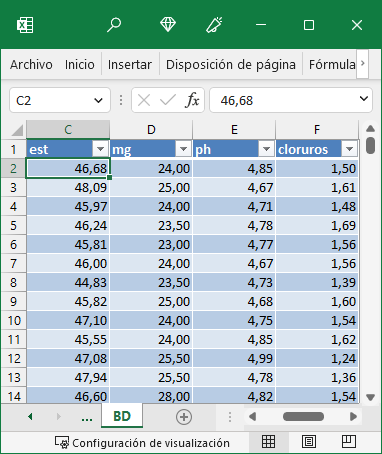
\includegraphics{01-imagenes/2023-01-20-1.png}

}

\caption{Tabla Excel}

\end{marginfigure}

Aunque en Excel no es fácil modificar esta estructura, R proporciona
herramientas muy útiles que permiten intercambiar filas o columnas, lo
que en ocasiones es muy útil en el análisis. Hadley Wickham (2017)
proporciona métodos detallados para manejar tablas de datos ordenados.

\hypertarget{de-excel-a-r}{%
\section{De Excel a R}\label{de-excel-a-r}}

Una vez que tenemos nuestros datos en Excel, hay dos formas en las que
podemos poner los datos a disposición de R para su análisis: exportarlos
a un archivo de texto con \textbf{\emph{formato CSV}}, o leer
directamente los datos de Excel desde R utilizando las funciones de la
librería \texttt{tidyverse}. En ambos casos, el resultado en R es un
\textbf{\emph{dataframe}} o \emph{cuadro de datos}, que es una
estructura equivalente a la de nuestra tabla de datos en Excel.

\hypertarget{quuxe9-es-un-fichero-plano-y-un-fichero-csv}{%
\subsection{Qué es un fichero plano y un fichero
CSV}\label{quuxe9-es-un-fichero-plano-y-un-fichero-csv}}

Se suele llamar \textbf{fichero plano} a un fichero de datos de texto
sin ningún tipo de formato, donde los datos están separados por espacios
o tabulaciones. Muchos equipos automáticos, como balanzas de laboratorio
o básculas de proceso, producen ficheros planos de texto, que se pueden
importar a Excel o R. Un
\href{https://es.wikipedia.org/wiki/Valores_separados_por_comas}{fichero
CSV} es un fichero plano en el que los valores están separados por un
carácter especial, llamado \textbf{separador}. Este separador puede ser
una coma \texttt{,} (cuando los decimales se separan mediante un punto,
como en EEUU) o un punto y coma \texttt{;} (cuando los decimales se
separan mediante una coma, como en España)

\begin{figure}

\begin{minipage}[b]{0.50\linewidth}

{\centering 

\raisebox{-\height}{

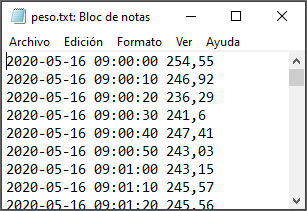
\includegraphics{01-imagenes/fichero-plano.png}

}

\caption{Fichero plano}

}

\end{minipage}%
%
\begin{minipage}[b]{0.50\linewidth}

{\centering 

\raisebox{-\height}{

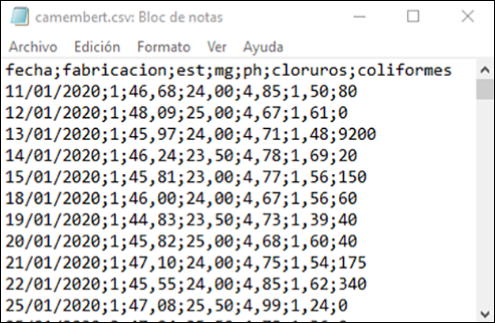
\includegraphics{01-imagenes/fichero-csv-europeo.png}

}

\caption{Fichero CSV separado por puntos y comas}

}

\end{minipage}%
\newline
\begin{minipage}[b]{\linewidth}

{\centering 

\raisebox{-\height}{

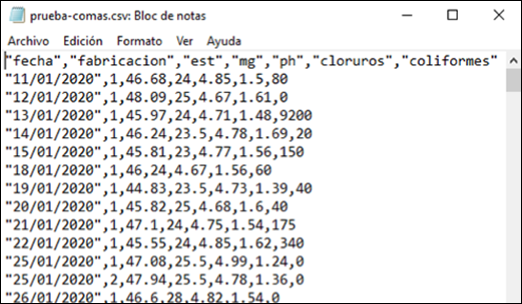
\includegraphics{01-imagenes/fichero-csv-comas.png}

}

\caption{Fichero CSV separado por comas}

}

\end{minipage}%

\caption{\label{fig-ficheros-texto}Tres tipos de ficheros planos de
texto.}

\end{figure}

En un fichero plano o en un fichero CSV, la primera fila puede contener
los nombres de las columnas. En algunos casos, los elementos de texto
pueden estar entre comillas. En estos casos, los programas de
importación se ocupan de la conversión de formatos.

La importación de un fichero CSV en Excel en español es directa si se ha
generado con puntos y comas como separador y comas para los decimales;
si no es así, nos aparecerá como un fichero plano de texto sin formato,
y tendremos que realizar una conversión.

\hypertarget{cuxf3mo-exportar-los-datos-a-un-fichero-csv-desde-excel.}{%
\subsection{Cómo exportar los datos a un fichero CSV desde
Excel.}\label{cuxf3mo-exportar-los-datos-a-un-fichero-csv-desde-excel.}}

\hypertarget{la-reproducibilidad-de-los-anuxe1lisis-de-datos}{%
\section{La reproducibilidad de los análisis de
datos}\label{la-reproducibilidad-de-los-anuxe1lisis-de-datos}}

\href{https://en.wikipedia.org/wiki/Literate_programming}{Literate
programming - Wikipedia}

\href{https://hbiostat.org/rr/\#reproducible-research-bbr-chapter-21}{Reproducible
Research (hbiostat.org)}

\href{https://hbiostat.org/rr/\#reproducible-research-bbr-chapter-21}{rr
(hbiostat.org)}

En el mundo científico y técnico cada vez cobra más importancia el
concepto de \textbf{reproducibilidad de los análisis}, sobre todo cuando
se trata de comunicar o publicar el resultado de un trabajo o de una
investigación. Medios, como la prestigiosa revista \emph{Science}, se
han hecho eco de ello (Buck 2015). Por otra parte, la utilización de un
flujo de trabajo basado en hojas de cálculo hace difícil garantizar esta
reproducibilidad, y a veces puede llevar a cometer errores de
consecuencias graves (Ferrero 2018; Ryssdal 2013).

Jesse Sadler (Sadler 2017) lo explica así:

\begin{quote}
El peligro de la hoja de cálculo deriva de su propia estructura. La
mezcla de entrada de datos, análisis y visualización hace que sea fácil
confundir las celdas que contienen datos sin procesar con las que son el
resultado del análisis. La forma de definir la lógica programática, tal
como la selección de qué celdas se van a sumar, mediante clics del
mouse, significa que una acción errónea de clic o arrastre puede
provocar errores o la sobreescritura de datos. Solo hace falta pensar en
el pavor del momento en el que vas a cerrar una hoja de cálculo y el
programa te pregunta si te gustaría guardar los cambios. Te hace
preguntarte. ¿Quiero guardar? ¿Qué cambios hice? Debido a que la lógica
en una hoja de cálculo se realiza a través de clics del mouse, no hay
forma de rastrear de manera efectiva qué cambios se han realizado en una
sesión o en la producción de un gráfico. Los errores cometidos con Excel
pueden tener consecuencias graves, como se puso de manifiesto tras la
controversia alrededor del
\href{https://nadaesgratis.es/garicano/el-error-de-reinhardt-y-rogoff}{artículo
de Carmen Reinhart y Kenneth Rogoff} sobre la deuda nacional de los
EEUU.
\end{quote}

\begin{quote}
Ciertamente hay razones legítimas por las que las personas usan por
defecto hojas de cálculo para el análisis de datos en lugar de usar un
lenguaje de programación como R. Las hojas de cálculo son mucho más
atractivas y confortables de lo que cualquier lenguaje de programación
podría ser para un recién llegado. Aprender a programar es intimidante y
no es algo que se pueda hacer rápida o fácilmente. Las aplicaciones de
interfaz gráfica de usuario (GUI) son mucho menos desalentadoras que una
interfaz de línea de comandos. En segundo lugar, las hojas de cálculo
son una buena herramienta para la entrada de datos, y es tentador pasar
directamente al análisis de datos, manteniendo todo en el mismo
documento. Finalmente, la naturaleza interactiva de las hojas de cálculo
y la capacidad de crear gráficos que cambian en función de las entradas
es muy atractiva, incluso si desbloquear completamente este potencial
implica un conocimiento bastante complejo sobre cómo funciona el
programa. La primera ventaja de las hojas de cálculo sobre la
programación no se supera fácilmente, pero las dos últimas se basan en
lo que creo que es un flujo de trabajo problemático. En lugar de usar un
par de aplicaciones monolíticas, a menudo un conjunto de aplicaciones de
oficina, para hacer todo, creo que es mejor dividir el flujo de trabajo
entre varias aplicaciones que hacen una cosa bien.
\end{quote}

\begin{quote}
Crear una división clara entre la entrada y el análisis de datos es una
de las principales razones por las que el análisis de datos en un
lenguaje de programación es preferible al software de hoja de cálculo.
Todavía uso hojas de cálculo, pero su limito su uso estrictamente a la
entrada de datos. En un programa de hoja de cálculo, el análisis
manipula directamente la única copia de los datos sin procesar. Por el
contrario, con R se importan los datos, creando un objeto que es una
copia de los datos sin procesar. Todas las manipulaciones de los datos
se realizan en esta copia, y los datos originales nunca se alteran de
ninguna manera. Esto significa que no hay forma de estropear los datos
sin procesar. La manipulación de una copia de los datos le permite
experimentar más libremente. Los errores son intrascendentes, incluso
aunque a veces puedan llegar a ser frustrantes. Una línea de código que
devuelve un error se puede ajustar y volver a ejecutar, repitiendo el
proceso las veces necesarias hasta que se devuelva el resultado
esperado.
\end{quote}

\begin{quote}
Trabajar en una copia de los datos sin procesar puede incluso
simplificar el proceso de entrada de datos. El análisis de datos
tabulares en R da como resultado la creación de múltiples objetos, que
se conocen como \emph{data frames} y pueden considerarse equivalentes a
tablas en una hoja de cálculo. La capacidad de dividir, muestrear y
transformar el conjunto de datos original en muchos \emph{data frames}
diferentes tiene la ventaja de reducir drásticamente la complejidad de
la entrada de datos. En lugar de necesitar hojas de cálculo a medida con
múltiples hojas y tablas interrelacionadas, cada pieza de datos solo
debe ingresarse una vez y todas las manipulaciones se pueden realizar en
el código. Los diferentes \emph{data frames} que se crean en el proceso
de análisis ni siquiera tienen que ser guardados, porque son muy
fácilmente reproducidos por el script de código.
\end{quote}

\begin{quote}
La separación de la entrada y el análisis de los datos reduce en gran
manera el potencial de errores, pero tal vez aún más significativamente,
el uso de código para el análisis de datos permite la creación de
investigaciones reproducibles que no son posibles en hojas de cálculo.
{[}\ldots{]} Con un lenguaje de programación, los pasos del análisis se
pueden establecer claramente en el código {[}\ldots{]} Guardar el
análisis en código tiene el beneficio inmediato de que se puede volver a
ejecutar fácilmente en cualquier momento que se agreguen nuevos datos.
El código también se puede aplicar a un conjunto de datos completamente
nuevo de una manera mucho más transparente que con las hojas de cálculo.
El beneficio a largo plazo es que con el código todo el análisis se
documenta en lugar de ocultarse detrás de los clics del mouse. Esto hace
que sea más fácil revisar los propios análisis mucho después de haber
terminado con ellos, así como que otros entiendan lo que se ha hecho y
comprueben si hay errores.
\end{quote}

\hypertarget{el-flujo-de-trabajo}{%
\section{El flujo de trabajo}\label{el-flujo-de-trabajo}}

\begin{itemize}
\item
  En qué consiste un flujo de trabajo en el análisis de datos

  Gráfico de R4DS

  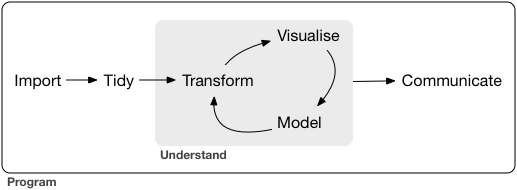
\includegraphics{01-imagenes/data-science.png}
\item
  Cómo estructurar un flujo de trabajo para el análisis de datos
  industriales
\end{itemize}

\hypertarget{el-uso-de-la-hoja-de-cuxe1lculo}{%
\section{El uso de la hoja de
cálculo:}\label{el-uso-de-la-hoja-de-cuxe1lculo}}

\begin{itemize}
\item
  Introducción y almacenar datos
\item
  Tablas dinámicas
\item
  Gráficos y edición gráfica
\end{itemize}

\hypertarget{el-uso-de-r}{%
\section{El uso de R}\label{el-uso-de-r}}

\begin{itemize}
\item
  Exploración de datos (gráficos básicos)
\item
  Manipulación de datos y exportación para su uso en Excel
\item
  Análisis estadísticos
\item
  Gráficos de control
\end{itemize}

Informes automatizados

\bookmarksetup{startatroot}

\hypertarget{los-datos-industriales-de-producciuxf3n}{%
\chapter{Los datos industriales de
producción}\label{los-datos-industriales-de-producciuxf3n}}

En el entorno industrial, los datos son recogidos casi siempre por uno
de estos tres caminos:

\begin{itemize}
\tightlist
\item
  Estudio retrospectivo, basado en datos históricos
\item
  Estudio observacional
\item
  Experimento diseñado
\end{itemize}

Un buen sistema de recogida de datos facilitará el estudio posterior. Si
ponemos poco cuidado en la toma de datos y en la forma de guardarlos,
nos encontraremos después con problemas complicados de resolver en la
fase de análisis o en la de interpretación , y, en algunos casos, estos
problemas serán imposibles de resolver.

\hypertarget{estudios-retrospectivos-o-histuxf3ricos}{%
\section{Estudios retrospectivos o
históricos}\label{estudios-retrospectivos-o-histuxf3ricos}}

Un \textbf{estudio retrospectivo o histórico} es el que utiliza una
muestra o todos los datos históricos de un proceso, recogidos en el
pasado durante un período determinado de tiempo. El objetivo de un
estudio de este tipo puede ser la investigación sobre la relación entre
algunas variables, o explorar la calidad de la información disponible, o
construir un modelo que permita explicar el proceso tal como es
actualmente, o saber si se ha desviado. Estos modelos del proceso se
denominan \textbf{modelos empíricos}, porque están basados en los
propios datos del proceso y no en una formulación teórica sobre el
mismo.

Un estudio retrospectivo tiene la ventaja de tener a su disposición un
gran número de datos que ya han sido recogidos, minimizando el esfuerzo
de obtenerlos. Sin embargo, tiene varios problemas potenciales:

\begin{enumerate}
\def\labelenumi{\arabic{enumi}.}
\tightlist
\item
  Si no disponemos de detalles suficientes, es posible que no podamos
  determinar si las condiciones de variación de los valores obtenidos
  responden a las mismas causas que en la situación actual.
\item
  Es posible que nos falte algún valor clave que no haya sido recogido o
  que lo haya sido de manera defectuosa
\item
  Algunas veces, la fiabilidad y validez de los datos de proceso
  históricos son dudosas, o al menos, cuestionables.
\item
  Los datos históricos no siempre se han recogido con la perspectiva
  actual del proceso, y es posible que no nos proporciones explicaciones
  adecuadas del proceso en su situación actual.
\item
  A veces queremos utilizar los datos históricos de proceso para fines
  que no estaban previstos cuando se recogieron
\item
  Las notas sobre los valores del proceso, incluyendo los valores
  anormales, pueden ser insuficientes o inexistentes, y no tenemos
  ninguna explicación sobre los posibles valores anómalos que detectamos
  en el análisis.
\end{enumerate}

Usar datos históricos siempre tiene el riesgo de que, por la razón que
sea, no se hayan recogido datos importantes, o que estos datos se hayan
perdido, o se hayan transcrito de forma inadecuada o incorrecta. Es
decir, los datos históricos pueden tener problemas de calidad de datos.

El hecho de que algunos datos se hayan recogido históricamente no
siempre quiere decir que estos datos sean relevantes o útiles. Cuando el
grado de conocimiento del proceso no es suficiente, o no se basa en un
análisis metódico y riguroso de los datos, es posible que no se hayan
recogido algunos datos que pueden ser importantes para el proceso, a
veces simplemente porque son complejos o difíciles de analizar. Los
datos históricos no pueden proporcionar la información que buscamos si
la información de las variables clave nunca se ha recogido o se ha hecho
sin una buena base experimental.

El propósito del análisis de los datos industriales es aislar las causas
que están detrás de los sucesos que afectan e influyen en los procesos.
En los datos históricos, estos sucesos pueden haber ocurrido semanas,
meses o incluso años antes, sin que haya registros ni notas que hayan
intentado explicar estas causas, y los recuerdos de las personas que han
participado en ellos se pierden con el tiempo, o se alteran
involuntariamente, proporcionando explicaciones supuestamente válidas
pero que en realidad son incorrectas. Por eso, con frecuencia, el
análisis de los datos históricos puede poner de manifiesto hechos
interesantes, pero sus causas quedan sin explicar.

Los estudios históricos pueden requerir una fase previa de preparación y
depuración de datos que puede llegar a ser muy larga y tediosa. Se
estima que en muchos estudios de ciencia de datos, el tiempo de
preparación de los datos puede llegar al \(60\%\) del tiempo total
empleado en el estudio. Las herramientas de análisis de datos son de
gran ayuda en esta fase del proceso, aunque en muchas ocasiones será
necesario un trabajo manual de recolección de datos en papel, hojas de
cálculo diversas y otras fuentes. Esta fase es muy útil no sólo para la
preparación de datos para el estudio, sino para mejorar el conocimiento
de los datos, cómo se originan y cómo se almacenan. Este conocimiento
siempre es de gran utilidad para mejorar los procedimientos actuales de
captura de datos, facilitando la fiabilidad de los análisis futuros.

\hypertarget{estudios-observacionales}{%
\section{Estudios observacionales}\label{estudios-observacionales}}

Como su nombre indica, un \textbf{estudio observacional} simplemente
observa un proceso durante un tiempo de operación en rutina.
Normalmente, el ingeniero o técnico interfiere lo mínimo posible en el
proceso, sólo lo suficiente para recoger la información que necesita,
que en muchas ocasiones no forma parte de los controles de rutina, si
piensa que esa información puede ser relevante. Si se planifican
adecuadamente, los estudios observacionales proporcionan datos fiables,
precisos y completos para documentar un proceso. Por otra parte, estos
estudios proporcionan una información limitada sobre las relaciones
entre las variables del proceso, porque es posible que durante el tiempo
limitado de observación, el rango de variación de las variables no
recoja todas las situaciones posibles, incluyendo situaciones
extraordinarias.

\hypertarget{experimentos-diseuxf1ados}{%
\section{Experimentos diseñados}\label{experimentos-diseuxf1ados}}

{\marginnote{\begin{footnotesize}Factores
experimentales\end{footnotesize}}}

La tercera forma de recoger información de un proceso son los
\textbf{experimentos diseñados}. En un experimento de este tipo, el
ingeniero o técnico hace un cambio deliberado en las variables que
controla (llamadas \textbf{factores}), observa el resultado, y toma una
decisión respecto a qué variable o variables son responsables de los
cambios que observa en el proceso.

Una diferencia importante respecto a los estudios históricos y los
observacionales es que las diferentes combinaciones de factores se
aplican al azar sobre un conjunto de unidades experimentales. Esto
permite establecer con precisión las relaciones causa-efecto, cosa que
no suele ser posible en los estudios históricos ni en los
observacionales.

\bookmarksetup{startatroot}

\hypertarget{la-exploraciuxf3n-de-los-datos}{%
\chapter{La exploración de los
datos}\label{la-exploraciuxf3n-de-los-datos}}

\hypertarget{describiendo-un-conjunto-de-datos}{%
\section{Describiendo un conjunto de
datos}\label{describiendo-un-conjunto-de-datos}}

Supongamos que queremos medir la altura de los alumnos de nuestra clase.
nuestro analista de la OMS ha realizado la medida de la altura de una
niña siguiendo rigurosamente el método establecido, y, por lo tanto, que
está razonablemente seguro de su resultado.

Al cabo de varias jornadas de trabajo, habrá realizado varias medidas,
que representarán al conjunto de niños de la población en la que ha
estado trabajando. Otros investigadores pueden haber estado trabajando a
la vez en otras poblaciones, y al final de sus jornadas de trabajo,
quieren comparar sus resultados: ¿Hay alguna de estas poblaciones en las
que los niños sean significativamente más altos (o más bajos) que en las
otras? ¿Cómo describir la altura de un conjunto de individuos de manera
que se puedan hacer comparaciones con otros conjuntos?

Para responder a estas preguntas, vamos a cambiar el entorno de trabajo
a un grupo de niños imaginario, que vamos a llamar \emph{aula1}: son
nuestros compañeros y compañeras, a los cuales realizaremos una medida
de altura siguiendo el \emph{procedimiento} especificado en nuestro
\emph{método}.

Éste es nuestro grupo de estudiantes:

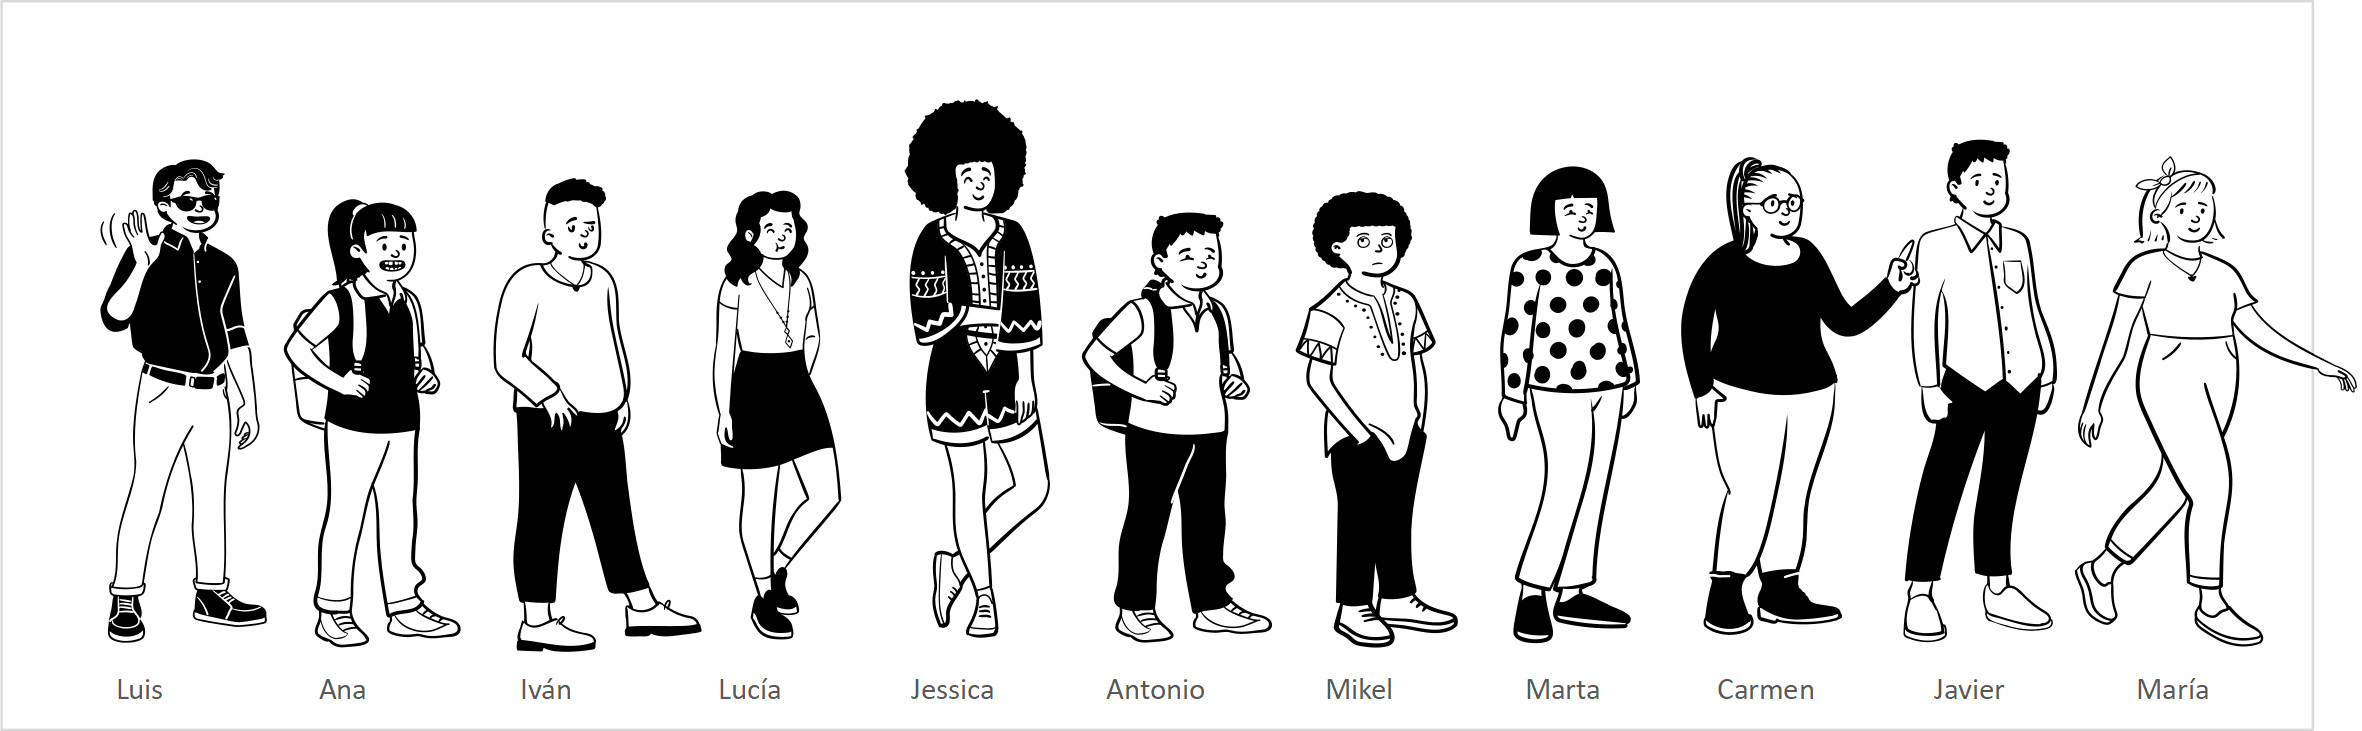
\includegraphics{01-imagenes/grupo1.jpg}

Supongamos que hemos realizado las medidas. Lo primero que hacemos es
registrar la altura de cada persona en una hoja de cálculo:

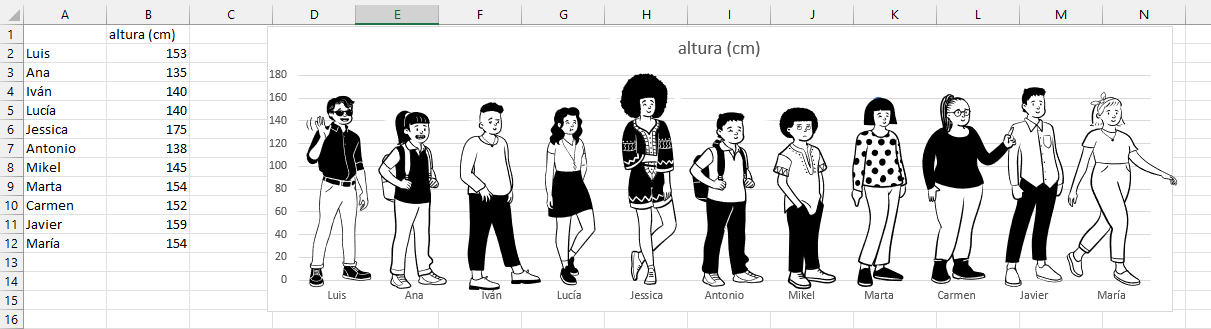
\includegraphics{01-imagenes/aula1(2).png}

\hypertarget{el-diagrama-de-puntos-o-dotplot}{%
\section{\texorpdfstring{El diagrama de puntos o
\emph{dotplot}}{El diagrama de puntos o dotplot}}\label{el-diagrama-de-puntos-o-dotplot}}

El diagrama de tallo y hojas

Construcción en Excel

\hypertarget{la-distribuciuxf3n-de-frecuencias}{%
\section{La distribución de
frecuencias}\label{la-distribuciuxf3n-de-frecuencias}}

Si agrupamos nuestros valores por intervalos, y contamos el número de
observaciones que aparecen en cada intervalo, obtenemos una
\emph{distribución de frecuencias}, que puede ser \emph{absoluta} o
\emph{relativa} según que sus valores sean un recuento simple de los
valores o el porcentaje que corresponde al número de observaciones en
cada clase respecto al total de observaciones

Las formas más habituales de representar una distribución de frecuencias
son la tabla de frecuencias o bien un gráfico de barras o histograma.

El gráfico a continuación muestra una distribución de frecuencias
absoluta, calculada mediante una tabla dinámica de Excel, junto con su
tabla de frecuencias absolutas.

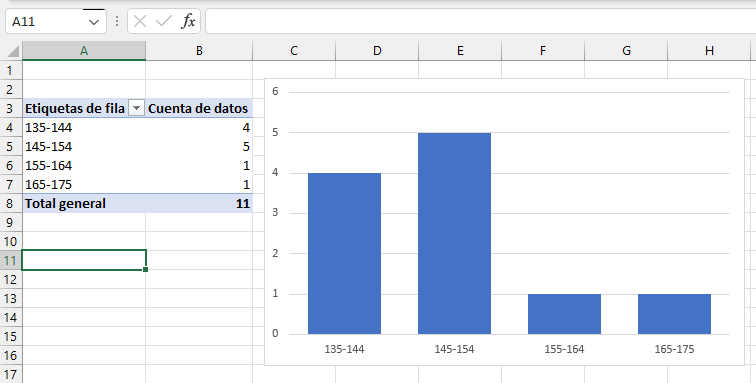
\includegraphics{01-imagenes/image-20221115205524355.png}

\href{https://www.fharrell.com/post/rflow/\#descriptive-statistics}{Statistical
Thinking - R Workflow (fharrell.com)}

Tables can summarize frequency distributions of categorical variables,
and measures of central tendency, selected quantiles, and measures of
spread for continuous variables. When there is a truly discrete baseline
variable one can stratify on it and compute the above types of summary
measures. Tables fail completely when one attempts to stratify on a
continuous baseline variable after grouping it into intervals. This is
because categorization of continuous variables
\href{https://discourse.datamethods.org/t/categorizing-continuous-variables}{is
a bad idea}. Among other problems,

\begin{itemize}
\tightlist
\item
  categorization misses relationships occurring in an interval (this
  happens most often when an interval is wide such as an outer quartile)
\item
  categorization loses information and statistical power because
  within-interval outcome heterogeneity is ignored and between-interval
  ordering is not utilized
\item
  intervals are arbitrary, and changing interval boundaries can
  significantly change the apparent relationship
\item
  with cutpoints one can easily manipulate results; one can find a set
  of cutpoints that results in a positive relationship and a different
  set
  \href{https://www.tandfonline.com/doi/abs/10.1080/09332480.2006.10722771}{that
  results in a negative relationship}
\end{itemize}

\hypertarget{diagramas-de-barra}{%
\section{Diagramas de barra}\label{diagramas-de-barra}}

\hypertarget{histogramas}{%
\section{Histogramas}\label{histogramas}}

\hypertarget{gruxe1ficos-de-densidad}{%
\section{Gráficos de densidad}\label{gruxe1ficos-de-densidad}}

\hypertarget{los-valores-centrales-media-mediana-moda}{%
\section{Los valores centrales: media, mediana,
moda}\label{los-valores-centrales-media-mediana-moda}}

\hypertarget{los-valores-de-dispersiuxf3n-varianza-y-desviaciuxf3n-tuxedpica-rango-intercuartil}{%
\section{Los valores de dispersión: varianza y desviación típica, rango
intercuartil}\label{los-valores-de-dispersiuxf3n-varianza-y-desviaciuxf3n-tuxedpica-rango-intercuartil}}

\hypertarget{diagramas-de-caja-box-plot}{%
\section{\texorpdfstring{Diagramas de caja (\emph{box
plot})}{Diagramas de caja (box plot)}}\label{diagramas-de-caja-box-plot}}

\href{https://www.leansigmacorporation.com/box-plot-with-minitab/}{Box
Plot with Minitab - Lean Sigma Corporation}

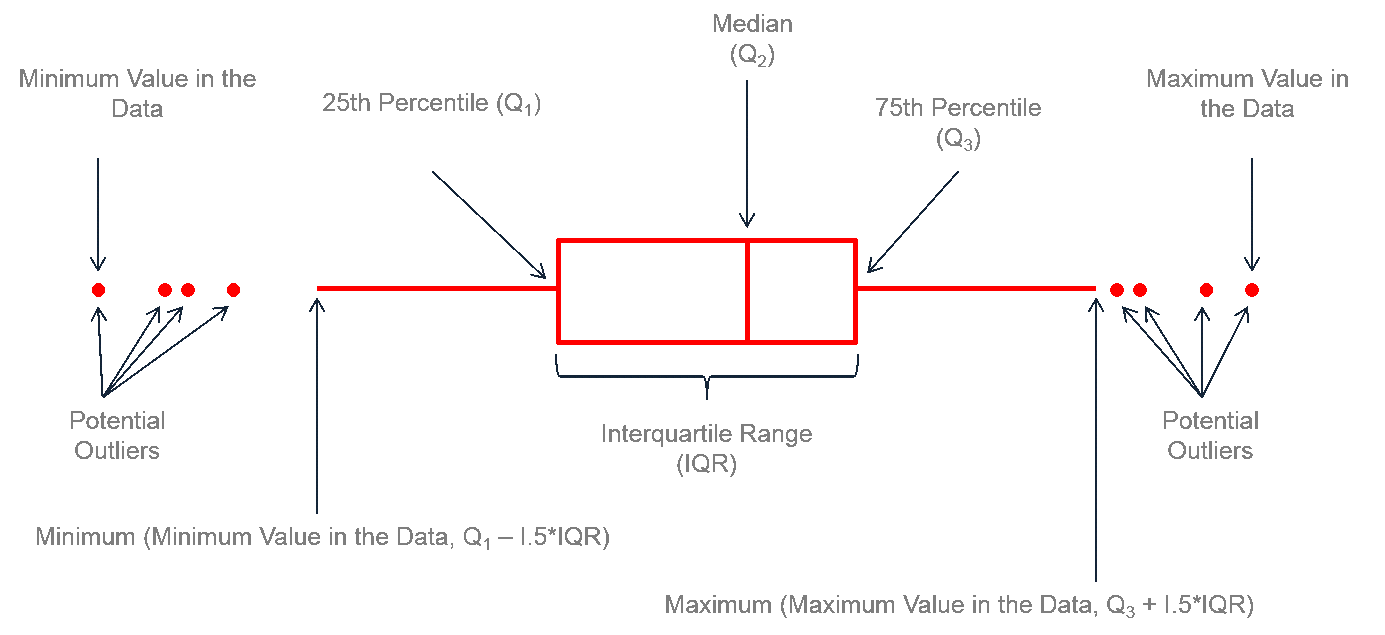
\includegraphics{01-imagenes/boxplot-minitab.png}

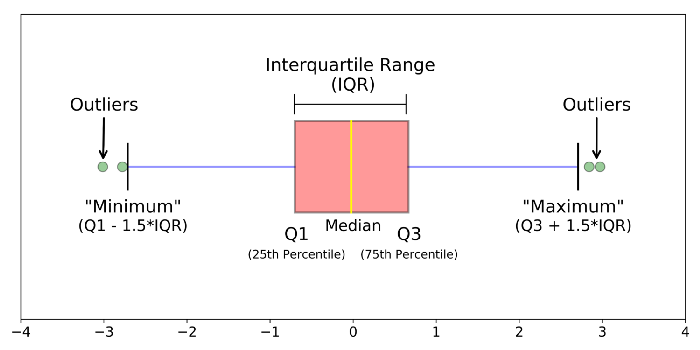
\includegraphics{01-imagenes/boxplot.png}

\href{http://r-graph-gallery.com/boxplot.html}{Boxplot \textbar{} the R
Graph Gallery (r-graph-gallery.com)}

\hypertarget{gruxe1ficos-de-series}{%
\subsection{Gráficos de series}\label{gruxe1ficos-de-series}}

\hypertarget{otros-gruxe1ficos}{%
\subsection{Otros gráficos}\label{otros-gruxe1ficos}}

dotplot

\href{https://ggplot2.tidyverse.org/reference/geom_dotplot.html}{Dot
plot --- geom\_dotplot • ggplot2 (tidyverse.org)}

\hypertarget{la-media-o-promedio-una-medida-central}{%
\subsection{La media o promedio: una medida
central}\label{la-media-o-promedio-una-medida-central}}

Una primera posibilidad es suponer que en nuestro grupo de once personas
no hubiese variación: que todos ellos tuviesen la misma altura. Si fuese
así, podemos encontrar un valor \(x\) de altura que, repetido once
veces, sea equivalente a la suma de las alturas de todos ellos. Si
representamos cada alumno con una letra, la suma de sus alturas sería:
\[
a+ b + c + d + e + f + g + h + i + j + k
\] y el valor que buscamos sería un valor tal que, sumado once veces, el
valor obtenido fuese igual a la suma de la alturas medidas: \[
a+b+c+d+e+f+g+h+i+j+k = x+x+x+x+x+x+x+x+x+x+x
\] Pero sabemos que la suma de valores repetidos es igual al valor
multiplicado por el número de repeticiones: \[
a+b+c+d+e+f+g+h+i+j+k = 11 x
\] Sólo tenemos que despejar la \(x\) para hallar este valor: \[
x = \frac{a+b+c+d+e+f+g+h+i+j+k}{11}
\] Este valor que hemos obtenido es lo que se conoce como \(media\),
\(valor{\ }medio\) o \(promedio\), y, como hemos visto, \textbf{es aquel
valor tal que repetido tantas veces como individuos tenemos, es
equivalente a la suma de los valores que hemos obtenido}. La media de
una muestra se representa habitualmente mediante el símbolo \[\bar{x}\],
y, de una manera más formal, su valor se obtiene mediante la fórmula
siguiente: \[
{\bar{x}={\frac {1}{n}}\sum _{i=1}^{n}x_{i}}
\] El signo \(\sum\) se conoce como \emph{sumatorio}, e indica que ese
término consiste en la suma de los \(x\) valores desde el primero hasta
el valor \(n\). Expresado mediante una formulación matemática,

\[
{\bar{x}={\frac {1}{n}}\sum _{i=1}^{n}x_{i}={\frac {x_{1}+x_{2}+\cdots +x_{n}}{n}}}
\] lo quiere quiere decir: \emph{``la suma de todos los valores
observados dividido entre el número de estos valores''}.

La \textbf{media} es lo que conocemos como un \emph{valor central}, ya
que representa el centro de nuestro conjunto de números. Como es el
centro de nuestro conjunto de datos, \emph{equidista} de todos los
valores, o lo que es lo mismo, la suma de las distancias de todos los
valores a este valor central es \(cero\). Más adelante veremos la
importancia de este hecho, al hablar de la dispersión y las formas de
cálculo de la misma. La \emph{media}, junto con otras medidas como la
\emph{mediana} y la \emph{moda} se conocen en estadística como
\textbf{medidas de tendencia central}. Como hemos dicho, la media de una
\textbf{muestra} se representa como \(\bar{x}\), mientras que la media
de una \textbf{población} se representa con la letra griega \emph{mu}:
\(\mu\). En ambos casos, el cálculo se realiza de forma idéntica.

Volvamos a nuestro ejemplo para realizar los cálculos según el modelo
que hemos descrito. En nuestro caso, la \emph{altura media} de nuestros
alumnos (la \emph{media} de nuestro conjunto de números) se calcula
como: \[
\bar{x} = \frac{153+135+140+140+175+138+145+154+152+159+154}{11} = 149,54
\] Utilicemos una hoja de cálculo para guardar nuestros valores.

La fórmula para obtener la media en la hoja de cálculo, por ejemplo en
la versión en español de \emph{Microsoft Excel}, es
\texttt{=PROMEDIO(...)}, donde los puntos suspensivos deben sustituirse
por el rango a calcular. En nuestro ejemplo, introduciríamos la fórmula
en la celda \texttt{B13}como \texttt{=PROMEDIO(B2..B12)} (Para más
detalles, verificar la hoja Excel adjunta).

Para representar más cómodamente nuestros valores, dibujamos un punto a
la altura de cada alumno,

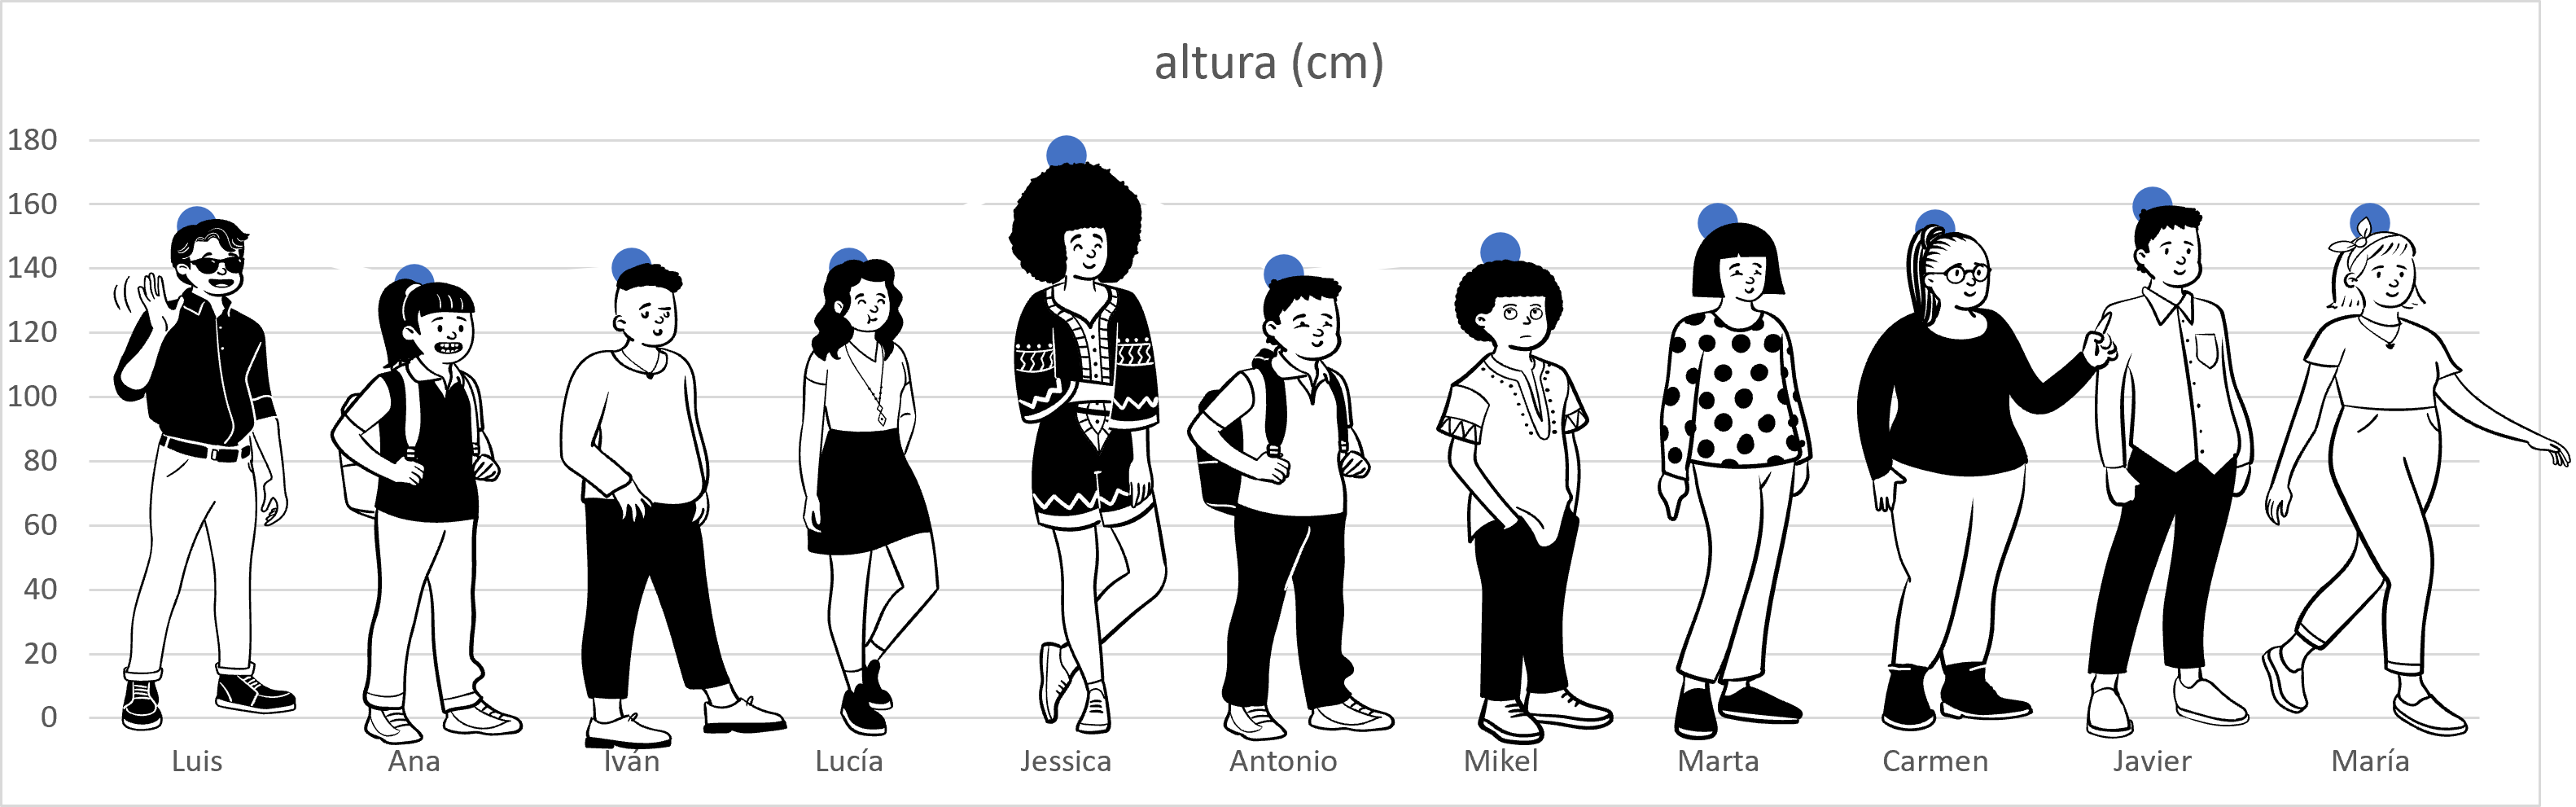
\includegraphics{D:/Usuarios/Juan/OneDrive/Documentos/010 Formación/001-Libro estadistica/01-imagenes/aula1_puntos-1.png}

y eliminamos del gráfico los dibujos de nuestros alumnos; así hemos
convertido nuestro dibujo en un \emph{diagrama de puntos}:

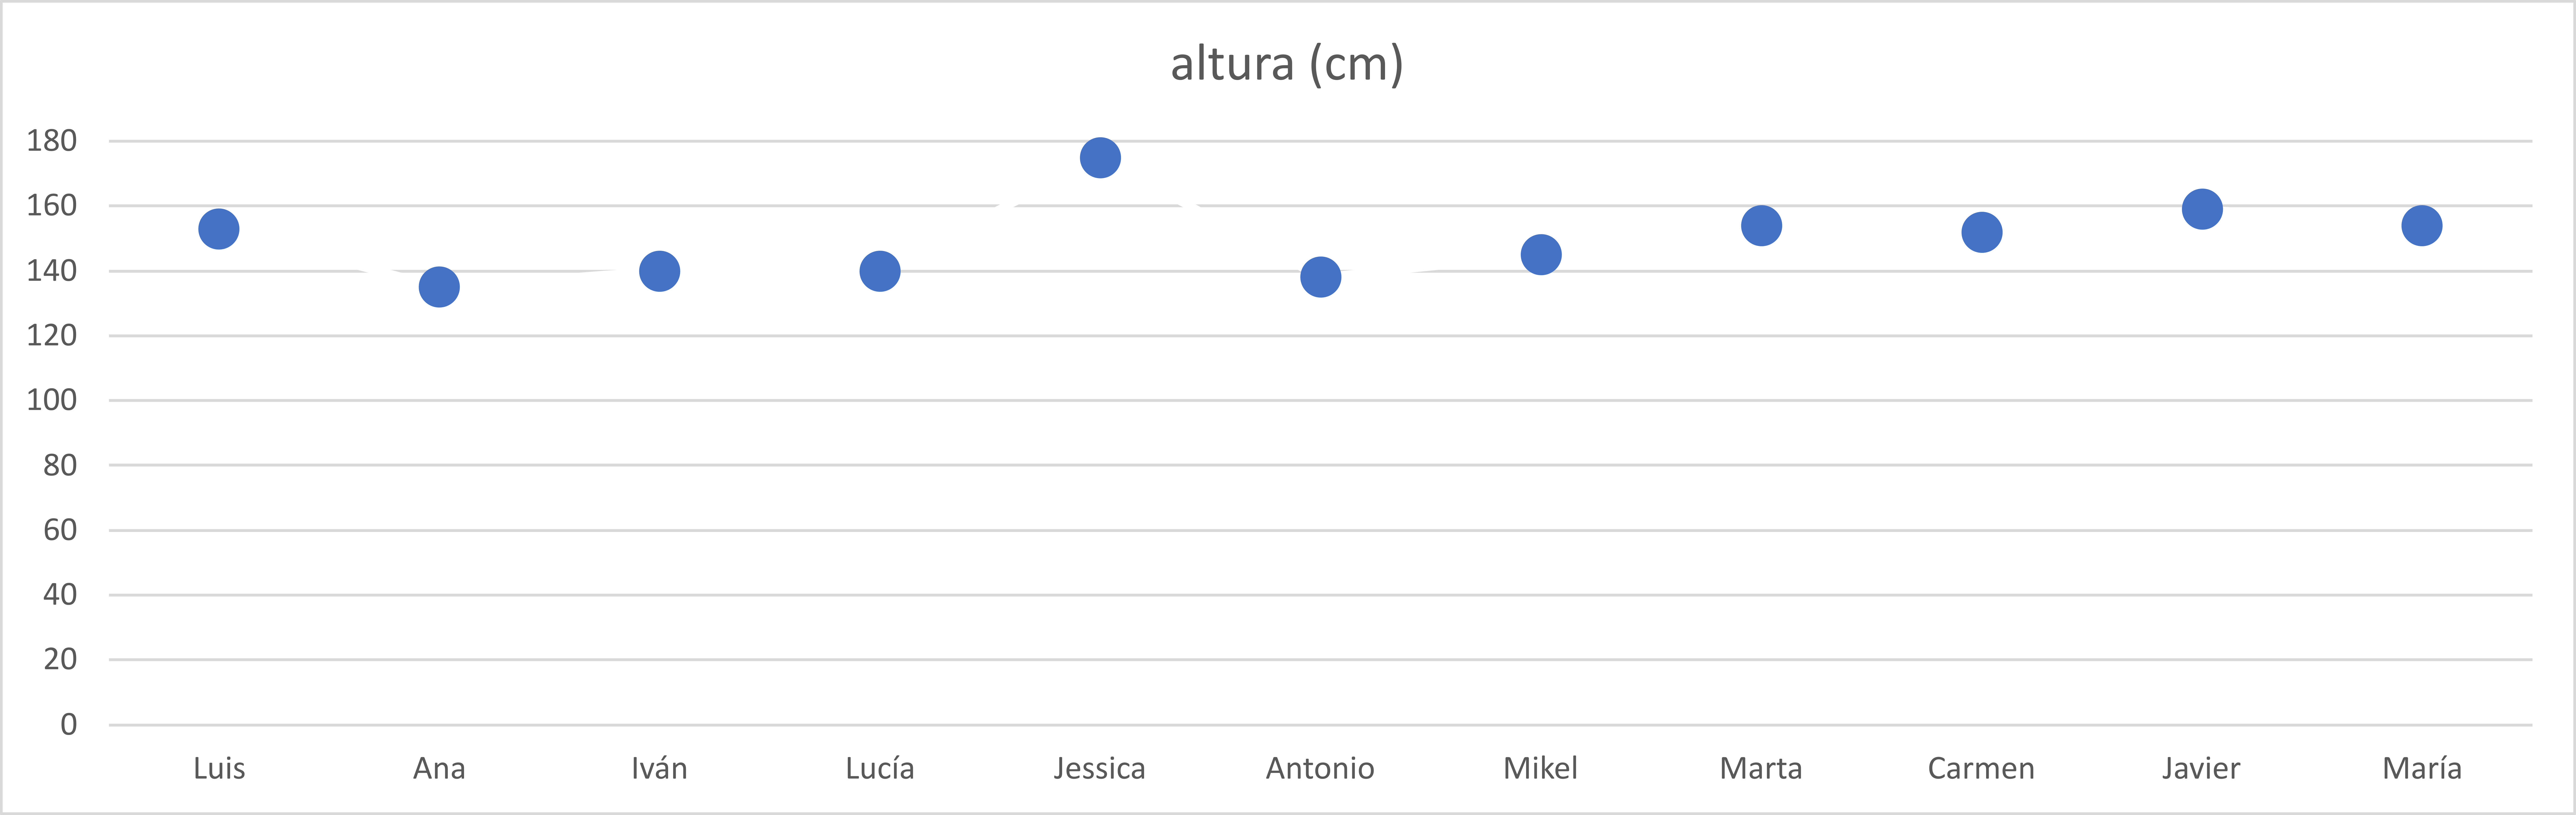
\includegraphics{D:/Usuarios/Juan/OneDrive/Documentos/010 Formación/001-Libro estadistica/01-imagenes/aula1_puntos.png}

Para representar la media, aunque la media es un valor único,
necesitamos añadir una columna a la derecha de nuestros datos, que
rotulamos en la fila 1, celda C como \texttt{altura\ media}, e
introducimos en cada una de las celdas desde \texttt{C2}hasta
\texttt{C12}la fórmula del promedio, con le valor de nuestro rango de
datos (Verificar hoja de cálculo). A continuación, designamos nuestro
rango de datos para hacer un gráfico de puntos, y hacemos un \emph{zoom}
en los valores de manera que el eje Y se escale mejor entre los valores
mínimo y máximo. Por último, hacemos unos ajustes en el formato para
dibujar las líneas verticales que nos representan la distancia de cada
valor a la media.

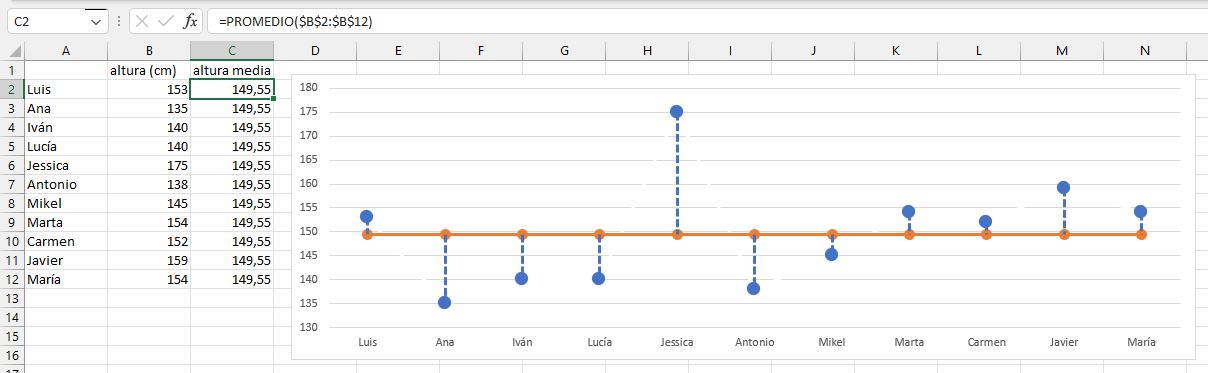
\includegraphics{D:/Usuarios/Juan/OneDrive/Documentos/010 Formación/001-Libro estadistica/01-imagenes/image-20221115203450170.png}

Si verificamos el eje \(Y\) , veremos que en este gráfico hemos ajustado
la escala respecto al gráfico anterior, situando el mínimo en \(130\).
Esto permite visualizar las diferencias con mucha más claridad. Hemos
representado la media \(\bar{x}\) como una línea, y hemos dibujado unas
líneas que unen cada valor individual con la media, que se sitúa en el
valor \(149,55\), tal como calculamos más arriba.

Hemos representado la media como una serie de puntos unidos por una
línea amarilla. Tal como hemos visto cuando hacíamos la descripción de
este parámetro, representamos un conjunto de valores idénticos, ya que
según hemos visto, la media \textbf{es aquel valor tal que repetido
tantas veces como individuos tenemos, es equivalente a la suma de los
valores reales que hemos obtenido}

Representamos en azul nuestros valores, uniendo cada valor con la línea
media mediante una línea de puntos vertical. A partir de ahora, por
conveniencia, eliminaremos los puntos en la linea media, dejando sólo la
línea.

\begin{figure}

{\centering 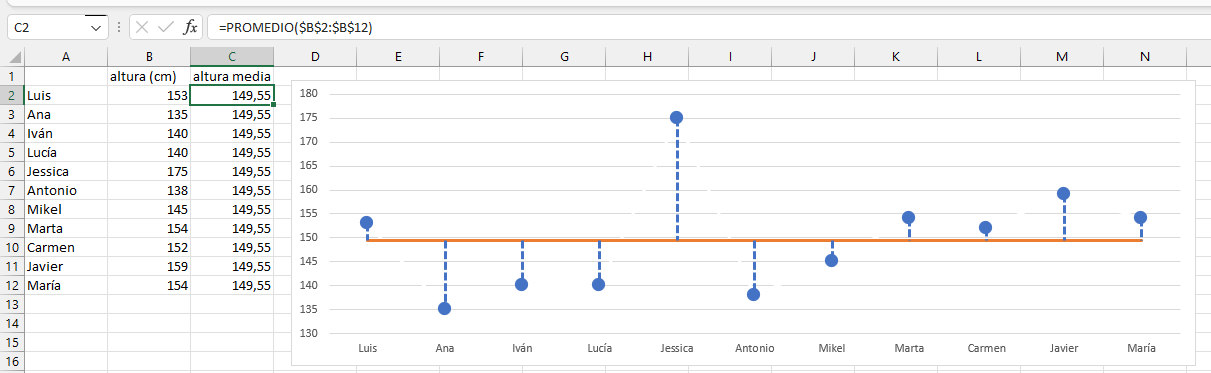
\includegraphics{D:/Usuarios/Juan/OneDrive/Documentos/010 Formación/001-Libro estadistica/01-imagenes/image-20221115202048866.png}

}

\caption{Hoja de cálculo con los valores y el gráfico de puntos}

\end{figure}

Esta línea azul de puntos representa la \emph{distancia} de cada valor a
la media. Usaremos esta distancia para calcular una \emph{distancia
media}, que será una medida de la dispersión de nuestros valores.

Recordemos que estamos intentando encontrar la forma de describir
nuestro conjunto de números con un valor, con el fin de que nuestros
analistas de la OMS puedan comparar la información de diferentes grupos
de niños y ayudara determinar su situación nutricional.

Hemos visto que para describir un conjunto de números, en nuestro
ejemplo, las medidas de la altura de un grupo de estudiantes, existe un
valor, la \emph{media} de este conjunto, que nos describe el centro de
los valores. En nuestro ejemplo, si nuestro grupo tuviese un solo niño,
éste tendría \(149,55{\ }cm\) de altura.

¿Es suficiente con este valor para describir el conjunto de valores?
Vamos a ver que no: diferentes conjuntos de valores pueden proporcionar
el mismo \emph{valor medio}, y sin embargo los grupos pueden ser muy
diferentes.

Veamos un caso extremo. Comparemos dos grupos, uno formado por
individuos iguales y otro formado por diez individuos iguales y uno
distinto. Para ello usaremos nuestra hoja de cálculo:

\begin{marginfigure}

{\centering 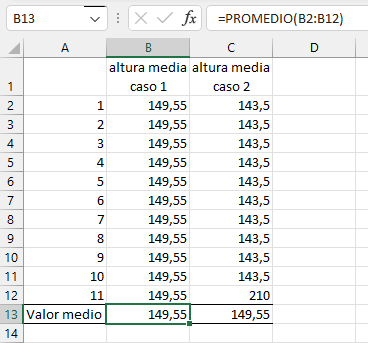
\includegraphics{D:/Usuarios/Juan/OneDrive/Documentos/010 Formación/001-Libro estadistica/01-imagenes/image-20221116105300331.png}

}

\caption{Dos grupos de valores con la misma media}

\end{marginfigure}

¿Podemos describir adecuadamente los valores de la altura de cada uno de
los grupos utilizando el valor medio? Parece evidente que no, ya que a
partir de diferentes valores de altura estamos obteniendo el mismo valor
medio. Sin embargo, uno de los grupos \emph{es más alto} que el otro, si
no fuera por un sólo individuo que aparentemente distorsiona el cálculo.
Podríamos incluir nuestro grupo original, y veremos que los tres grupos
son diferentes, aunque su valor medio es idéntico.

\begin{marginfigure}

{\centering 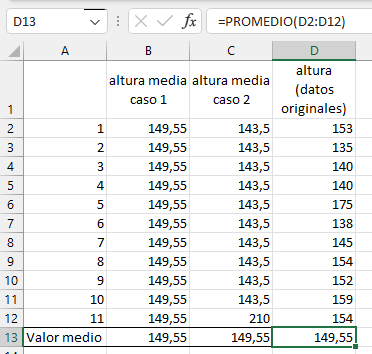
\includegraphics{D:/Usuarios/Juan/OneDrive/Documentos/010 Formación/001-Libro estadistica/01-imagenes/image-20221116110426263.png}

}

\caption{Tres grupos de valores con la misma media}

\end{marginfigure}

Si nos ayudamos de un gráfico equivalente al que hemos utilizado antes,
vemos estas diferencias con claridad:

\begin{figure}

{\centering 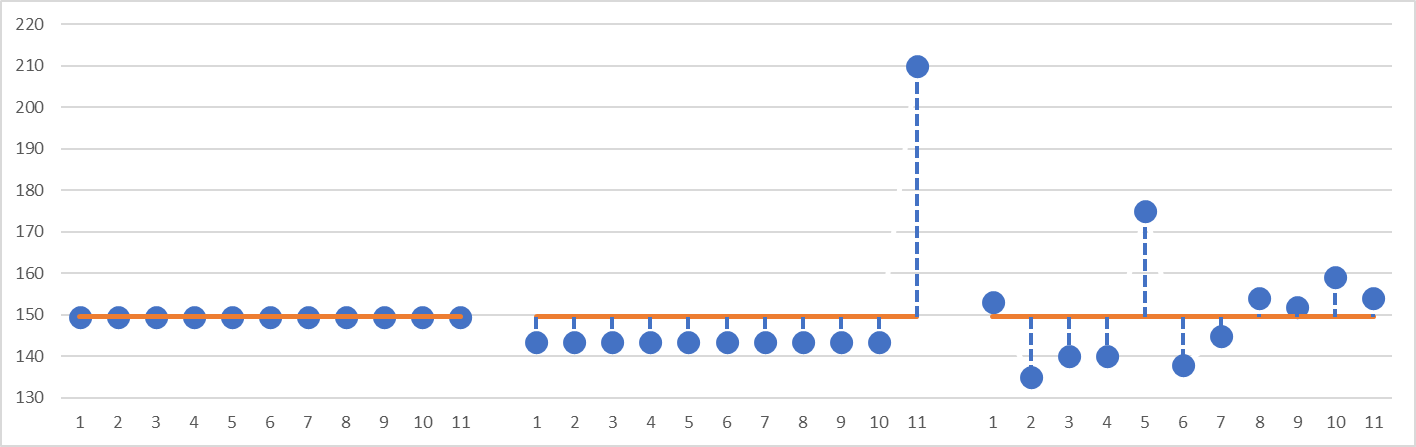
\includegraphics{D:/Usuarios/Juan/OneDrive/Documentos/010 Formación/001-Libro estadistica/01-imagenes/image-20221116110925933.png}

}

\caption{Gráfico de tres grupos de valores}

\end{figure}

Aunque el valor medio de estos tres grupos de datos es idéntico, parece
claro que los tres grupos son muy distintos en su composición, y por lo
tanto la \emph{media} no es suficiente para describir con suficiente
precisión cada uno de los grupos. Necesitamos un valor adicional, que
nos indique de qué forma los valores se alejan del valor medio. Para
ello, vamos a introducir un concepto nuevo: la \emph{medida de la
dispersión}, que nos indica precisamente la distancia de los valores al
valor medio, e introduciremos también la \emph{distribución de
frecuencias}, que nos permite representar \emph{la forma} en la que se
distribuyen nuestros valores.

La media como centro de gravedad:
\href{https://www.physicsclassroom.com/Physics-Interactives/Balance-and-Rotation/COM-Builder/Center-Of-Mass-Interactive}{Physics
Simulation: Center of Mass (physicsclassroom.com)}

\hypertarget{las-medidas-de-dispersiuxf3n-la-desviaciuxf3n-tuxedpica}{%
\subsection{Las medidas de dispersión: la desviación
típica}\label{las-medidas-de-dispersiuxf3n-la-desviaciuxf3n-tuxedpica}}

Como hemos visto en el apartado anterior, diferentes conjuntos de datos
pueden tener el mismo valor medio y sin embargo ser muy diferentes. En
la última gráfica que hemos visto, el primer grupo se caracteriza por
tener todos sus valores idénticos; el segundo tiene todos sus valores
idénticos menos uno, que está muy apartado del resto, y el tercero tiene
todos sus valores diferentes.

Ahora que conocemos cómo calcular un valor resumen de un conjunto de
datos, podríamos utilizar una medida semejante para describir de qué
forma en cada caso los valores se separan de la media. Podríamos
utilizar una \emph{distancia media}: calculamos las diferencias entre
cada valor y la media, y hacemos su promedio: esto debería darnos una
indicación de la magnitud de la separación de los valores en cada uno de
los tres grupos.

Usemos la hoja de cálculo para ello:

\begin{figure}

{\centering 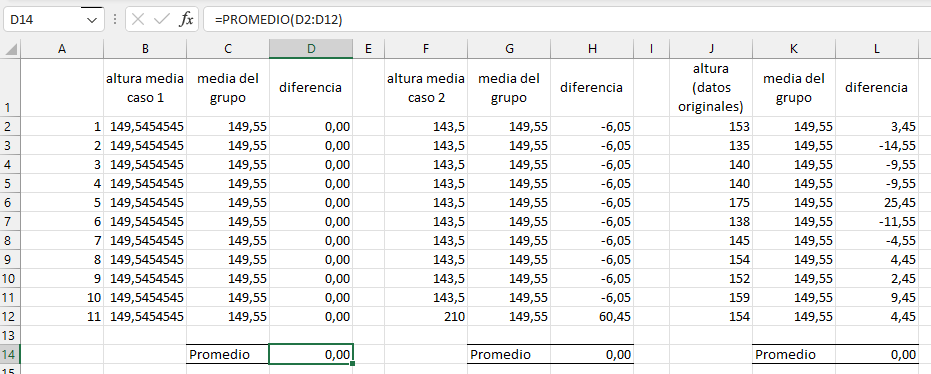
\includegraphics{D:/Usuarios/Juan/OneDrive/Documentos/010 Formación/001-Libro estadistica/01-imagenes/image-20221116113404185.png}

}

\caption{Tres grupos de valores en la hoja de cálculo}

\end{figure}

Algo parece que no está funcionando aquí: el promedio de las diferencias
es cero en los tres casos; no podemos usar este cálculo para calcular la
dispersión. Pero esto es esperable: ya que la media es un valor central,
como hemos visto antes, la suma de las diferencias de todos los valores
respecto de su media debe ser forzosamente cero, y esto es lo que
estamos obteniendo.

Para encontrar una solución, vamos a recurrir al viejo teorema de
Pitágoras, que si recuerdas, nos dice que, en un triángulo rectángulo,
el cuadrado de la hipotenusa es igual a la suma de los cuadrados de los
catetos (una explicación gráfica muy divertida en el anexo \ldots): \[
h^2= a^2+b^2
\] Esta fórmula es la base del cálculo de la distancia entre dos puntos:

\begin{marginfigure}

{\centering 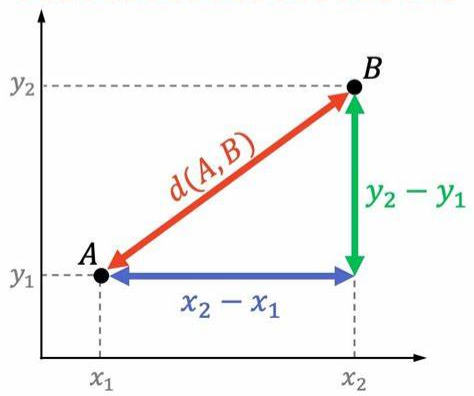
\includegraphics{D:/Usuarios/Juan/OneDrive/Documentos/010 Formación/001-Libro estadistica/01-imagenes/image-20221116114659713.png}

}

\caption{Distancia entre dos puntos}

\end{marginfigure}

\[
d(A,B)=\sqrt{(x_2-x_1)^2+(y_2-y_1)^2}
\] ¿Podemos adaptar esta fórmula para el cálculo de nuestra distancia
media? La respuesta es \textbf{sí}. En nuestro caso, sólo necesitamos la
coordenada \(X\), ya que sólo estamos calculando la distancia en una
dimensión. Si tenemos en cuenta un solo punto, esta distancia \(d\)
sería: \[
(d{\ }del{\ }valor{\ }1{\ }a{\ }la{\ }media)^2=(x_1-\bar{x})^2
\] ¡El hecho de elevar al cuadrado las diferencias nos da la solución!
Las diferencias negativas ya no son un problema porque sabemos que al
elevar un numero negativo al cuadrado, el resultado es positivo; de esta
manera conseguimos que las diferencias no se anulen. Ahora sí podemos
calcular una distancia media \(\bar{d}\) entre el conjunto de puntos y
su media, calculando el promedio de las diferencias elevadas al
cuadrado: \[
(\bar{d}{\ }de{\ }los{\ }n{\ }valores{\ }a{\ }la{\ }media)^2=\frac{(x_1-\bar{x})^2 + (x_2-\bar{x})^2+\cdots+(x_n-\bar{x})^2}{n}
\] y utilizando la notación que hemos aprendido antes, \[
(\bar{d}{\ }de{\ }los{\ }n{\ }valores{\ }a{\ }la{\ }media)^2={\frac {1}{n}}\sum _{i=1}^{n}(x_{i}-\bar{x})^2
\]

Al igual que en el cálculo de la distancia entre dos puntos, sólo
tenemos que extraer la raíz cuadrada de este valor para obtener la
distancia media, que es el parámetro que estábamos buscando.

La \[(\bar{d}{\ }de{\ }los{\ }n{\ }valores{\ }a{\ }la{\ }media)^2\] se
conoce en estadística como \textbf{varianza}, y su raíz cuadrada es lo
que se conoce como \textbf{desviación típica}. La varianza de una
población se representa en estadística con el signo de la letra griega
\emph{sigma} minúscula elevada al cuadrado, \(\sigma^2\), y la
desviación típica, mediante la letra \(\sigma\). En el caso de una
muestra, la varianza se representa como \(s_x^2\), y la desviación
típica, como \(s_x\). En nuestro caso, utilizaremos la primera notación;
más adelante veremos los conceptos de \textbf{población} y
\textbf{muestra} y explicaremos el concepto de \textbf{grados de
libertad}. Veremos también que la fórmula para el cálculo de la
desviación típica muestral es ligeramente diferente de la de su
equivalente poblacional, y explicaremos por qué.

Es importante resaltar que la desviación típica \emph{es una medida de
la distancia media de los valores de una población a su media}, y por lo
tanto tiene dimensión, la misma que las medidas originales. La varianza,
al estar elevada al cuadrado, no tiene una dimensión, o, mejor dicho,
tiene la de la medida al cuadrado.

Con estos nuevos hallazgos, recalculamos nuestra hoja de cálculo:

\begin{figure}

{\centering 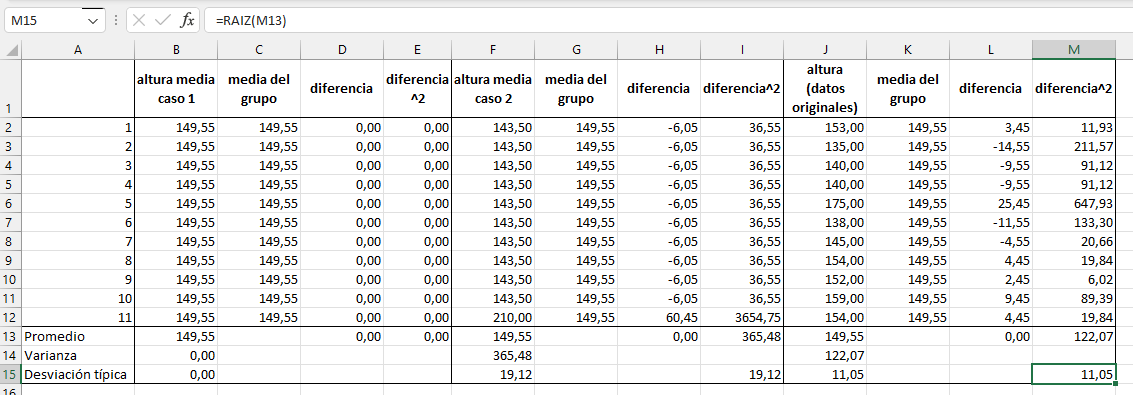
\includegraphics{D:/Usuarios/Juan/OneDrive/Documentos/010 Formación/001-Libro estadistica/01-imagenes/image-20221116123915941.png}

}

\caption{Tres grupos de valores en la hoja de cálculo, con la misma
media y distinta desviación típica}

\end{figure}

Vamos a analizar con detalle esta tabla.

En la columna \texttt{J} tenemos nuestra población original de 11
alumnos, con las alturas que hemos medido. En la columna \texttt{B}
hemos supuesto que todos los alumnos fuesen iguales, con la misma altura
del valor medio de los datos originales. En la columna \texttt{F} hemos
simulado otro grupo, con todos los valores iguales excepto uno, y con la
misma media que los otros dos grupos.

A la derecha de cada columna de medias, tenemos la columna de
diferencias (columnas \texttt{D}, \texttt{H} y \texttt{L}), y en la fila
\texttt{13}, nuestro primer intento de calcular una dispersión media;
intento fallido, puesto que obteníamos el valor \(0\) para los tres
grupos.

En la siguiente columna a la derecha, para los tres grupos (columnas
\texttt{E}, \texttt{I}y \texttt{M}), hemos elevado al cuadrado la
distancia de cada valor a la media, siguiendo los hallazgos que nos ha
proporcionado el teorema de Pitágoras y la fórmula de la distancia entre
dos puntos. En la fila \texttt{13} de estas columnas, calculamos el
promedio de la distancia a la media al cuadrado: esta vez el resultado
ya no es cero, sino que obtenemos el valor de la \textbf{varianza}, de
acuerdo con la fórmula que hemos deducido más arriba. En la fila
\texttt{14} (columnas B, \texttt{F} y \texttt{J})utilizamos la fórmula
de la hoja de cálculo para la \textbf{varianza poblacional} (más
detalles posteriormente), y vemos que coincide exactamente con el
promedio de las diferencias al cuadrado, tal como debe ser, ya que en
eso consiste la fórmula que hemos deducido.

Por último, en la fila \texttt{15}calculamos la desviación típica de
ambas formas, con la fórmula de la hoja de cálculo para la
\textbf{desviación típica poblacional} (columnas \texttt{B}, \texttt{F}y
\texttt{J}), que Excel llama \textbf{desviación estándar}, y como la
raíz cuadrada del promedio calculado antes (columnas \texttt{E},
\texttt{I}y \texttt{M}). De nuevo, ambos valores coinciden exactamente,
como esperamos.

\begin{figure}

{\centering 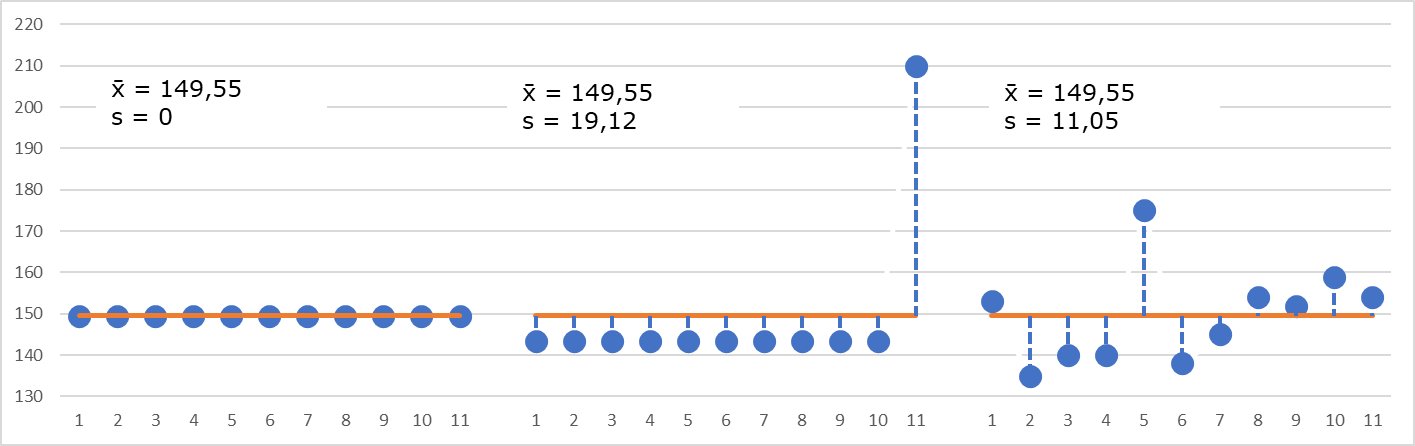
\includegraphics{D:/Usuarios/Juan/OneDrive/Documentos/010 Formación/001-Libro estadistica/01-imagenes/image-20221116135458643.png}

}

\caption{Gráfico con tres conjuntos de datos con la misma media y
diferente desviación típica}

\end{figure}

Ahora sí tenemos una forma más completa de describir nuestro conjunto de
valores. Aunque el valor medio es el mismo en los tres casos, la
\emph{dispersión} de los valores es muy distinta.

¿Son suficientes estos dos parámetros que hemos calculado para describir
un conjunto de datos? La respuesta a esta pregunta es sí y no. La
explicación es que, más allá de los valores numéricos que hemos
obtenido, la visualización gráfica de los valores nos debe hacer
reflexionar.

En el primer grupo, todos los valores son iguales a la media. La
variación es cero. Son valores que hemos simulado en nuestra hoja de
cálculo, pero difícilmente en el mundo real encontraremos una población
en la que todos sus valores, en este caso, la altura de un grupo de
alumnos, sean idénticos.

En el segundo grupo, todos los valores son idénticos, salvo uno, que se
distancia mucho. ¿Debemos aceptar esto como bueno? En realidad, ¿es
cierto que el valor medio de este grupo sea el mismo que el del primero?
Para responder a esta pregunta debemos recurrir a nuestra experiencia,
la estadística no nos da \emph{fórmulas mágicas}. Pero, con un poco de
sentido común, parece que el caso extremo que aparece en este grupo no
es coherente con el resto de valores. Es lo que se llama un \emph{valor
anormal} o \emph{extraño} (en inglés, \emph{outlier}), y debe hacernos
reflexionar sobre si el valor es correcto y realmente pertenece a esta
población, o es un error de medida. O, simplemente, un valor que
corresponde a otro grupo y que por error hemos situado en éste. La
decisión de eliminar o no un valor anormal es una de las decisiones más
complejas en estadística, que pueden tener una influencia enorme en la
interpretación de los datos, y por lo tanto, hay que hacer con sumo
cuidado. En este caso, extremo y artificial, el valor anormal debería
ser eliminado, ya que, en realidad, todos los valores restantes son
idénticos y más bajos que los del grupo 1. No tiene sentido lógico decir
que sus medias son idénticas.

En el tercer grupo todos los valores son diferentes, y no podemos decir
nada especial sobre sus valores individuales. Hay un valor que se
destaca del resto, pero ¿podemos afirmar que es anormal? Seguramente, no
con seguridad. De nuevo la experiencia debe indicarnos cómo proceder,
aunque en este caso no tendría sentido eliminar este valor. En la
situación real, todos conocemos a niños que han \emph{pegado el estirón}
antes que sus compañeros, y en algunos casos, pueden llegar a ser mucho
más altos (o más bajos, si han tenido un retraso en este \emph{estirón})
La experiencia nos dice que no es seguro que este valor sea realmente
anormal, y por lo tanto, deberíamos conservarlo.

\hypertarget{las-limitaciones-de-la-media-y-la-desviaciuxf3n-tuxedpica}{%
\subsection{Las limitaciones de la media y la desviación
típica}\label{las-limitaciones-de-la-media-y-la-desviaciuxf3n-tuxedpica}}

En ocasiones nos enfrentamos a conjuntos de datos con valores de media y
desviación típica idénticos o muy parecidos, pero que en realidad son
muy diferentes. Veamos un ejemplo, semejante a los que hemos visto hasta
ahora.

\begin{marginfigure}

{\centering 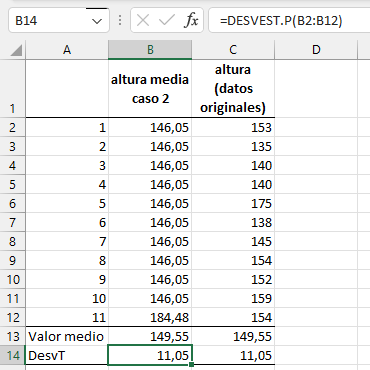
\includegraphics{D:/Usuarios/Juan/OneDrive/Documentos/010 Formación/001-Libro estadistica/01-imagenes/image-20221116164339577.png}

}

\caption{Hoja de cálculo con dos conjuntos de datos diferentes, con la
misma media y desviación típica}

\end{marginfigure}

(cambiar a caso 3)

\begin{figure}

{\centering 
\includegraphics{01-imagenes/media-balanza.png}

}

\caption{Diagrama de puntos de las alturas de los alumnos, con
indicación del valor medio}

\end{figure}

\begin{figure}

{\centering 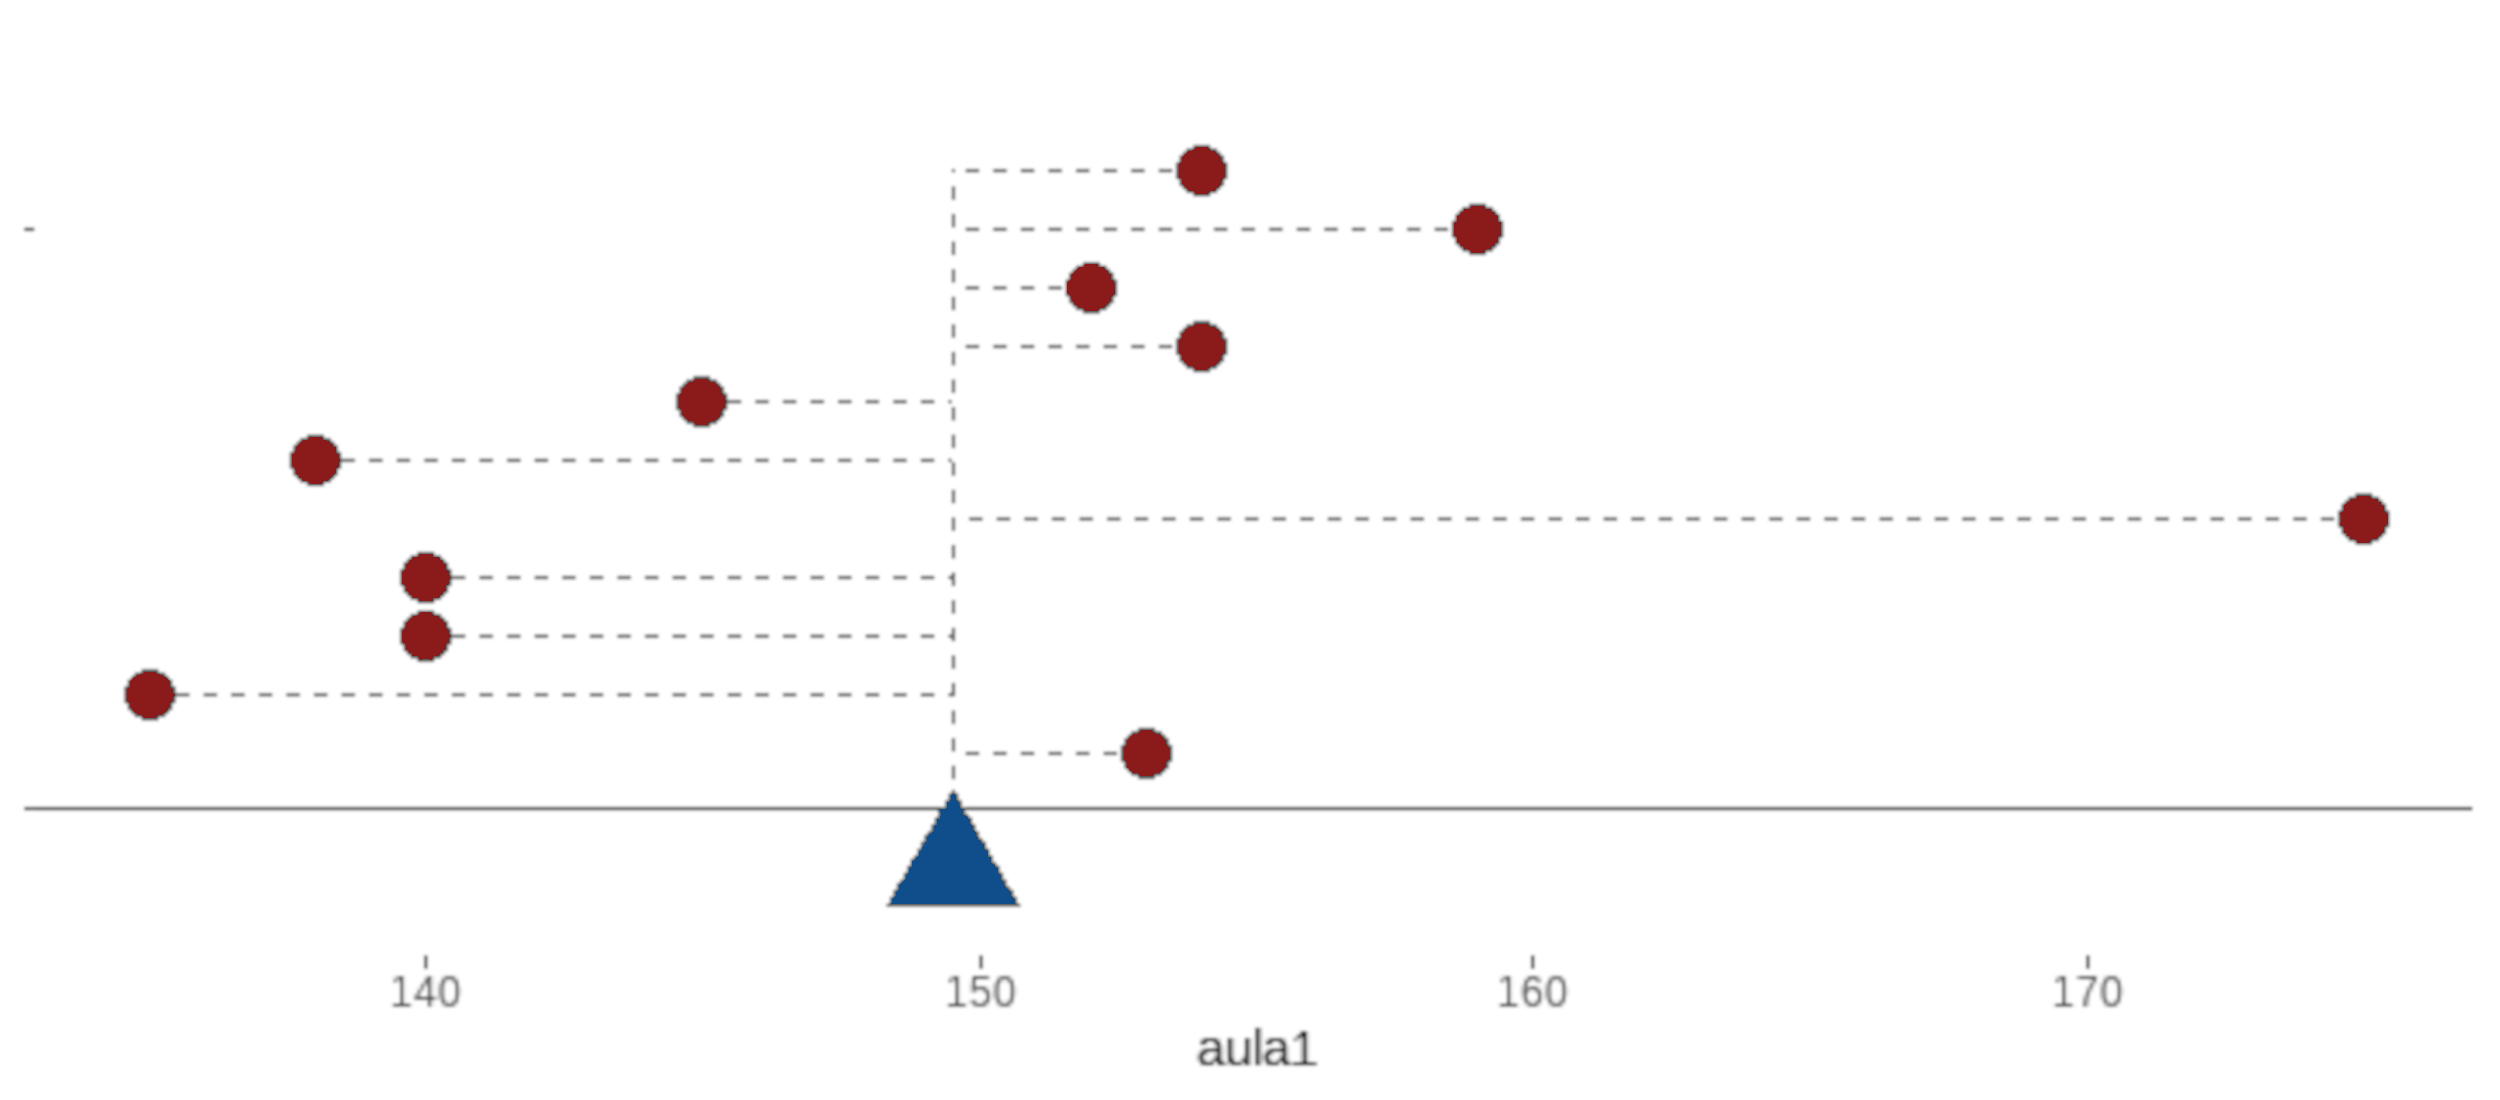
\includegraphics{01-imagenes/plot_varianzas.png}

}

\caption{Diagrama de puntos indicando la variabilidad}

\end{figure}

En este caso, vemos que tanto la media como la desviación típica son
idénticos, y sin embargo los datos son muy diferentes, tal como nos
muestra el gráfico de dispersión que hemos estado utilizando:

\begin{figure}

{\centering 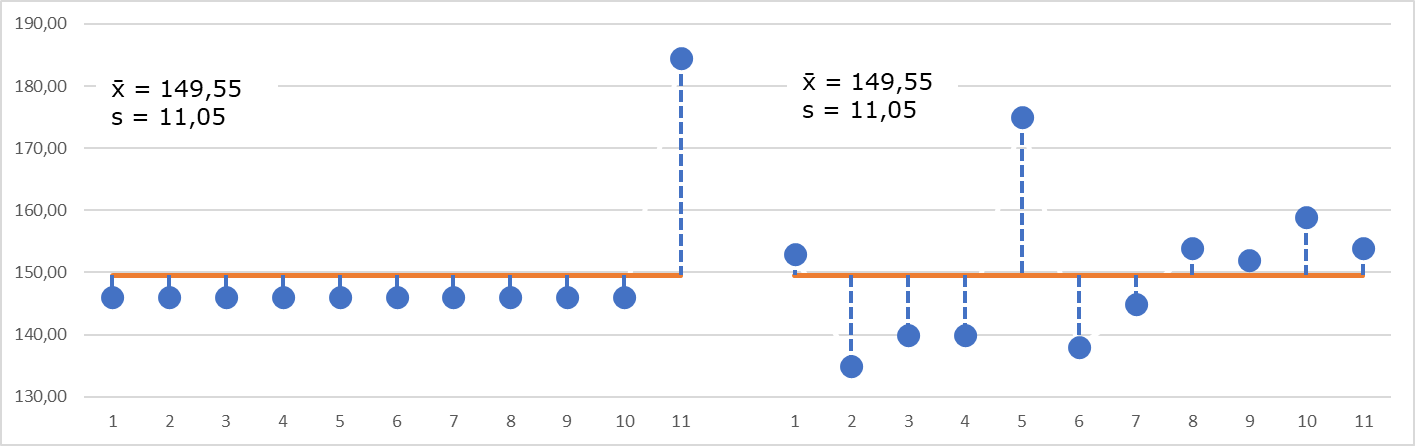
\includegraphics{D:/Usuarios/Juan/OneDrive/Documentos/010 Formación/001-Libro estadistica/01-imagenes/image-20221116164430210.png}

}

\caption{Gráfico con dos conjuntos de datos diferentes, con la misma
media y desviación típica}

\end{figure}

La existencia de valores anormales o extremos muestra una de las
debilidades de la media y la desviación típicas como \emph{descriptores}
de una población: ambos parámetros son muy sensibles a los casos
extremos. En realidad, sólo deberíamos utilizar la media y la desviación
típica para describir un conjunto de datos cuando estamos seguros de que
\emph{la distribución de estos datos} tienen una \emph{forma}
determinada, la de la \textbf{campana de Gauss}. Lo cual nos lleva al
siguiente capítulo: las \textbf{distribuciones de frecuencias}.

Modelo: práctica de puntos con un dado, dos dados, tres dados, etc hasta
30

suma \textless- rowSums(replicate(30, sample(6, 10\^{}6, replace=T)))
length(suma) hist(suma)

\href{http://sqljason.com/2018/12/financial-times-visual-vocabulary-power-bi-edition.html}{Financial
Times Visual Vocabulary: Power BI Edition -- Some Random Thoughts
(sqljason.com)}

\bookmarksetup{startatroot}

\hypertarget{distribuciones-de-probabilidad-e-inferencia}{%
\chapter{Distribuciones de probabilidad e
inferencia}\label{distribuciones-de-probabilidad-e-inferencia}}

\hypertarget{introducciuxf3n-al-concepto-de-probabilidad}{%
\section{Introducción al concepto de
probabilidad}\label{introducciuxf3n-al-concepto-de-probabilidad}}

\hypertarget{distribuciones-de-probabilidad}{%
\section{Distribuciones de
probabilidad}\label{distribuciones-de-probabilidad}}

\hypertarget{distribuciuxf3n-normal}{%
\subsection{Distribución normal}\label{distribuciuxf3n-normal}}

\href{https://www.economist.com/science-and-technology/2023/02/08/extreme-weather-events-are-getting-more-frequent}{How
to predict record-shattering weather events \textbar{} The Economist}

\begin{figure}

{\centering 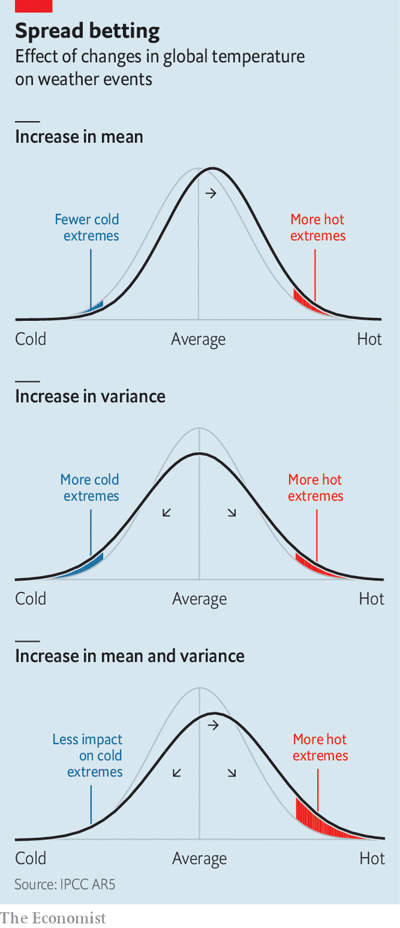
\includegraphics{01-imagenes/media-y-varianza.png}

}

\caption{media-y-varianza}

\end{figure}

\href{https://news.mit.edu/2012/explained-sigma-0209}{Explained: Sigma
\textbar{} MIT News \textbar{} Massachusetts Institute of Technology}

\begin{figure}

{\centering 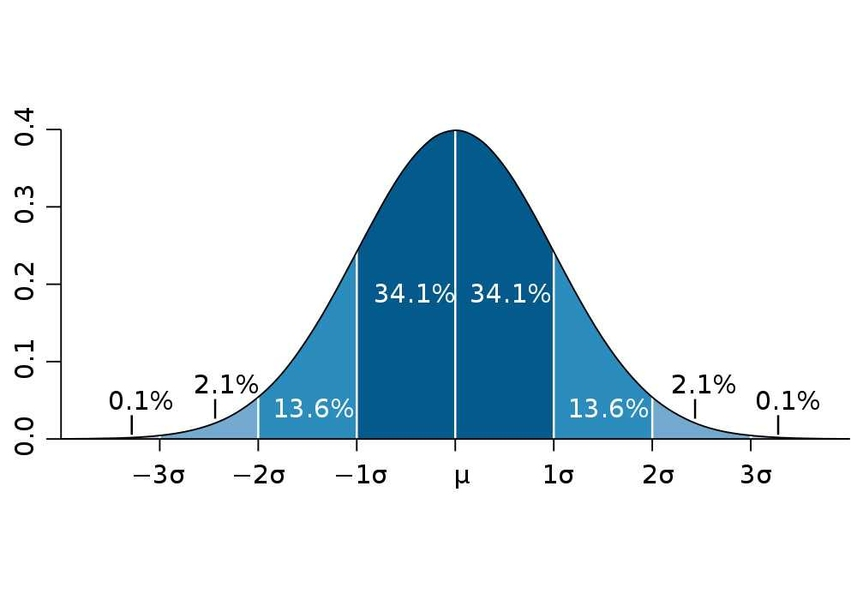
\includegraphics{01-imagenes/curva-normal.jpg}

}

\caption{img}

\end{figure}

\hypertarget{otras-distribuciones}{%
\subsection{Otras distribuciones}\label{otras-distribuciones}}

\hypertarget{gruxe1ficos-de-probabilidad}{%
\subsection{Gráficos de
probabilidad}\label{gruxe1ficos-de-probabilidad}}

\bookmarksetup{startatroot}

\hypertarget{la-relaciuxf3n-entre-las-variables}{%
\chapter{La relación entre las
variables}\label{la-relaciuxf3n-entre-las-variables}}

\hypertarget{diagramas-de-puntos-xy}{%
\section{\texorpdfstring{Diagramas de puntos
\((x,y\))}{Diagramas de puntos (x,y)}}\label{diagramas-de-puntos-xy}}

\hypertarget{correlaciuxf3n}{%
\section{Correlación}\label{correlaciuxf3n}}

\hypertarget{correlaciuxf3n-y-causalidad}{%
\subsection{Correlación y
causalidad}\label{correlaciuxf3n-y-causalidad}}

Anscombe

\hypertarget{tablas-de-asociaciuxf3n}{%
\section{Tablas de asociación}\label{tablas-de-asociaciuxf3n}}

\bookmarksetup{startatroot}

\hypertarget{el-anuxe1lisis-de-la-varianza}{%
\chapter{El análisis de la
varianza}\label{el-anuxe1lisis-de-la-varianza}}

\hypertarget{introducciuxf3n-1}{%
\section{Introducción}\label{introducciuxf3n-1}}

\hypertarget{anuxe1lisis-de-la-varianza-de-un-factor}{%
\section{Análisis de la varianza de un
factor}\label{anuxe1lisis-de-la-varianza-de-un-factor}}

\hypertarget{anuxe1lisis-de-la-varianza-de-dos-factores}{%
\section{Análisis de la varianza de dos
factores}\label{anuxe1lisis-de-la-varianza-de-dos-factores}}

\hypertarget{section}{%
\section{}\label{section}}

\bookmarksetup{startatroot}

\hypertarget{el-anuxe1lisis-del-sistema-de-mediciuxf3n}{%
\chapter{El análisis del sistema de
medición}\label{el-anuxe1lisis-del-sistema-de-mediciuxf3n}}

\hypertarget{quuxe9-es-una-medida}{%
\section{¿Qué es una medida?}\label{quuxe9-es-una-medida}}

Una medida es el resultado de la acción de \emph{medir}. Normalmente,
\emph{medir} quiere decir comparar lo que va a ser medido con un patrón
de referencia; esta comparación es realizada por una o varias personas
que llamaremos \emph{analistas}, los cuales utilizarán un \emph{método
analítico}, siguiendo un \emph{procedimiento de medida}. Por ejemplo, en
la imagen a continuación, la \emph{analista} está midiendo la altura de
un niño utilizando un \emph{instrumento de medida}, una cinta métrica.

\begin{marginfigure}

{\centering 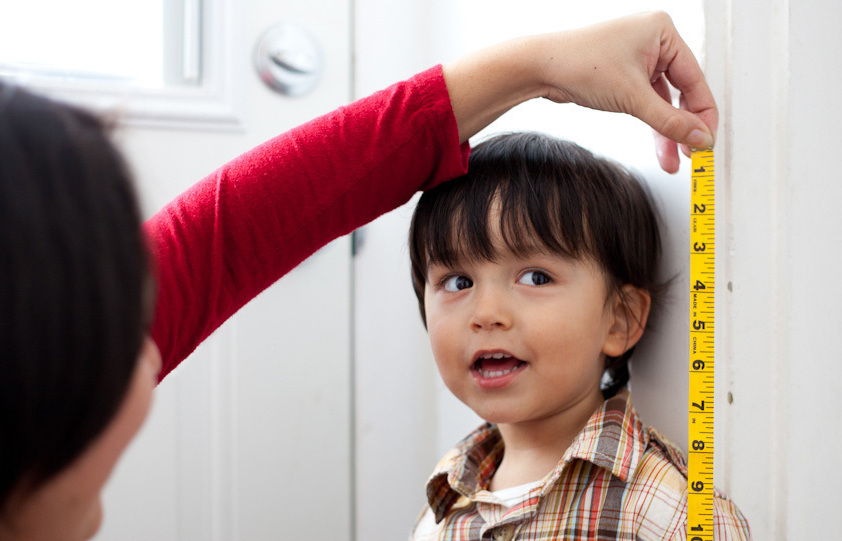
\includegraphics{D:/Usuarios/Juan/OneDrive/Documentos/010 Formación/001-Libro estadistica/01-imagenes/medida-altura.jpg}

}

\end{marginfigure}

Hasta aquí parece que todo está suficientemente claro, por lo que el
resultado de la medida debe ser un valor que no nos ofrecerá dudas sobre
su veracidad. Sin embargo, si analizamos el proceso con atención,
veremos que hay algunos elementos que pueden hacer que nuestro resultado
no sea todo lo preciso que habíamos pensado. Por ejemplo, en la imagen
no vemos si el niño está calzado o no. Es evidente que deberíamos decir
al analista que el niño debe estar descalzo, ya que diferentes tipos de
calzado podrían alterar el resultado de formas diferentes. EL niño
podría estar ligeramente encorvado, o sus rodillas dobladas, y entonces
la altura que estamos midiendo será menor de la altura real. Además de
esto, la forma de realizar la evaluación de la altura se ve influenciada
por la posición de los ojos del analista: si están demasiado bajos, no
verá correctamente la parte superior de la cabeza y tenderá a
sobreestimar el verdadero valor por un efecto de perspectiva. Por otra
parte, no sabemos si el instrumento utilizado tiene una escala de medida
construida de forma fiable o sólo aproximada. Si nuestro instrumento (la
cinta métrica) no es fiable, o su escala difiere de la de otros
instrumentos semejantes, es posible que el valor de la medida varíe.

\begin{marginfigure}

{\centering 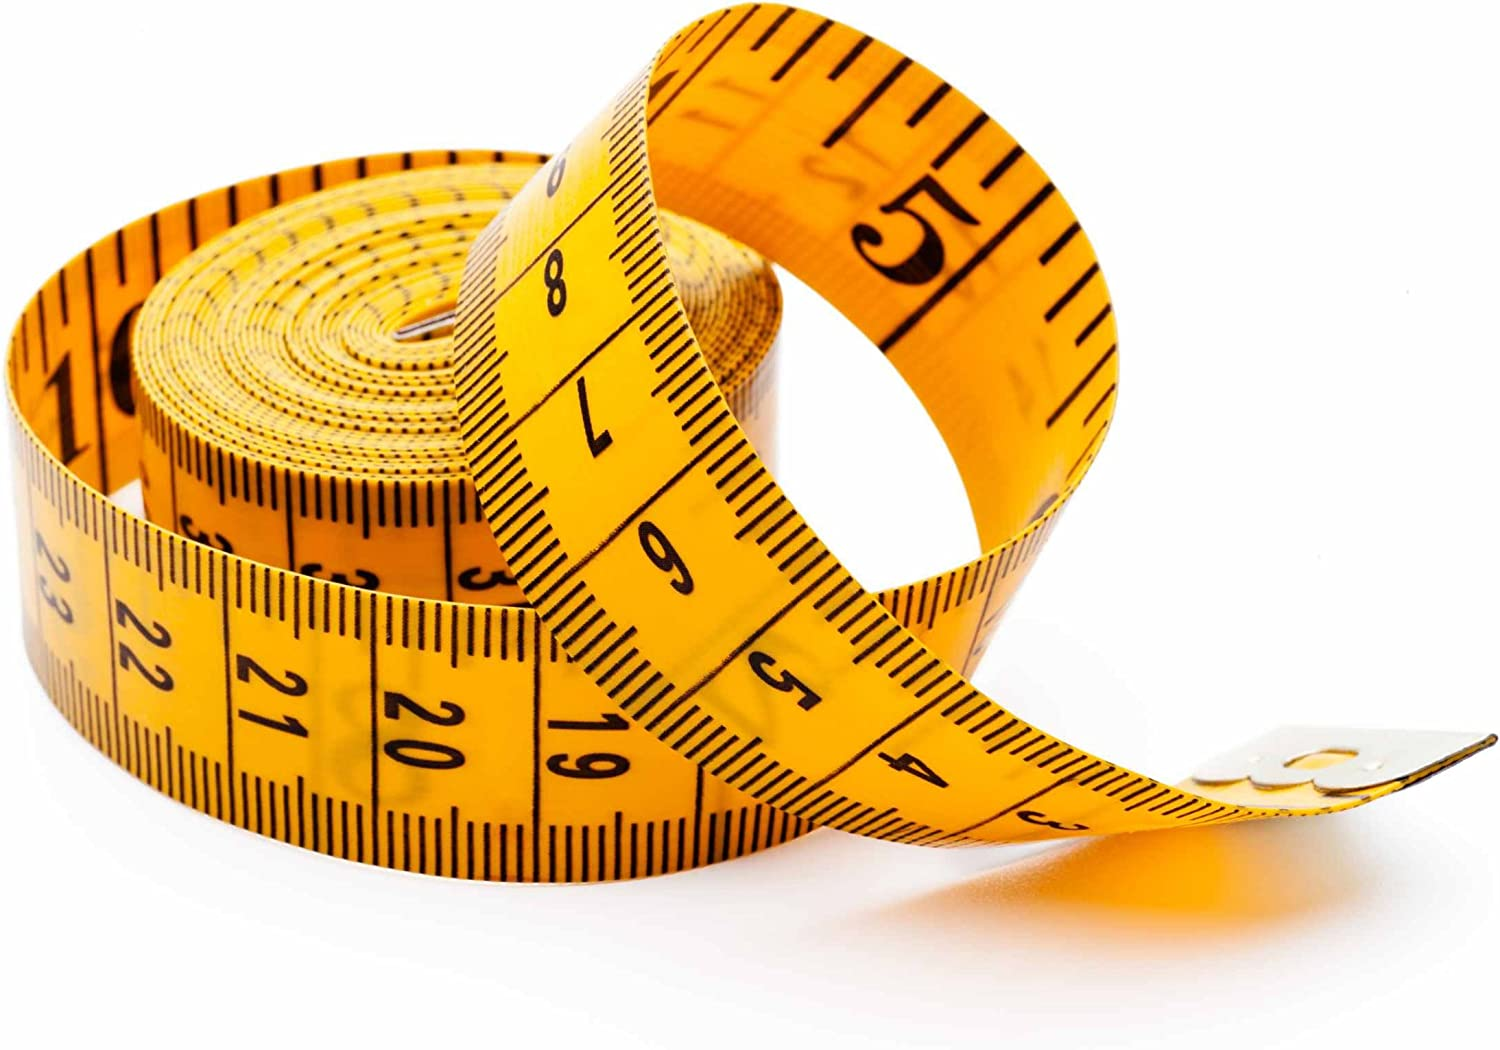
\includegraphics{D:/Usuarios/Juan/OneDrive/Documentos/010 Formación/001-Libro estadistica/01-imagenes/cinta_metrica_sastre_.jpg}

}

\caption{Cinta métrica de sastre}

\end{marginfigure}

\begin{marginfigure}

{\centering 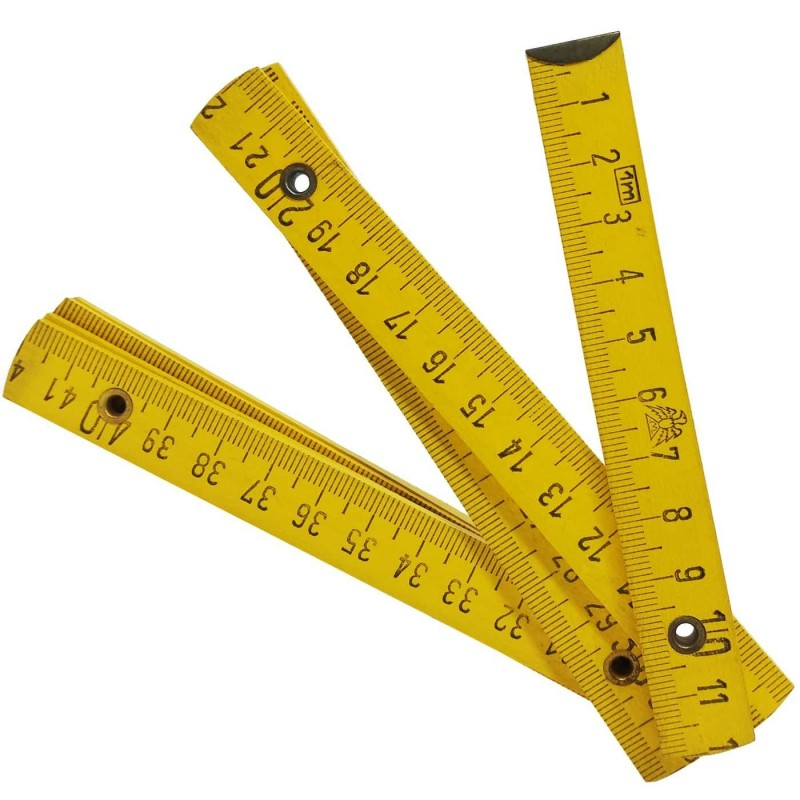
\includegraphics{D:/Usuarios/Juan/OneDrive/Documentos/010 Formación/001-Libro estadistica/01-imagenes/metro-carpintero-plegable-metro-de-albanil.jpg}

}

\caption{Metro de albañilería}

\end{marginfigure}

\hypertarget{los-estuxe1ndares-de-medida}{%
\section{Los estándares de medida}\label{los-estuxe1ndares-de-medida}}

Por lo que hemos visto, cuando hacemos una medida, debemos establecer un
\emph{procedimiento de medida}, que debe indicar al analista cual es la
forma correcta de realizar los pasos para hacer que la medida sea veraz.
Deberemos definir también el \emph{instrumento de medida}, de manera que
cuando se repita el procedimiento no se introduzca un factor de
variación debido al uno de un instrumento inapropiado. LO mejor es que
este instrumento disponga de una \emph{homologación} por un servicio de
homologación externo, que nos asegure, por ejemplo, que los intervalos
de medida de que dispone se corresponden con valores de referencia, en
este caso, centímetros y milímetros. El procedimiento debe establecer
también con claridad las condiciones en que las debe estar el objeto a
medir (la persona, en este caso): descalzo, perfectamente estirado, con
sus rodillas rectas, etc. Seguramente, el procedimiento incluirá un
dibujo para que el analista visualice con claridad los puntos claves que
debe revisar para hacer una buena medida. En el dibujo a continuación,
se indican algunos de estos puntos claves, incluyendo la necesidad de
que el niño se apoye en un plano vertical (la pared) y que el analista
se situe correctamente para que su vista sea perpendicular al plano,
utilizando una guía para la valoración correcta de la altura medida.

\begin{marginfigure}

{\centering 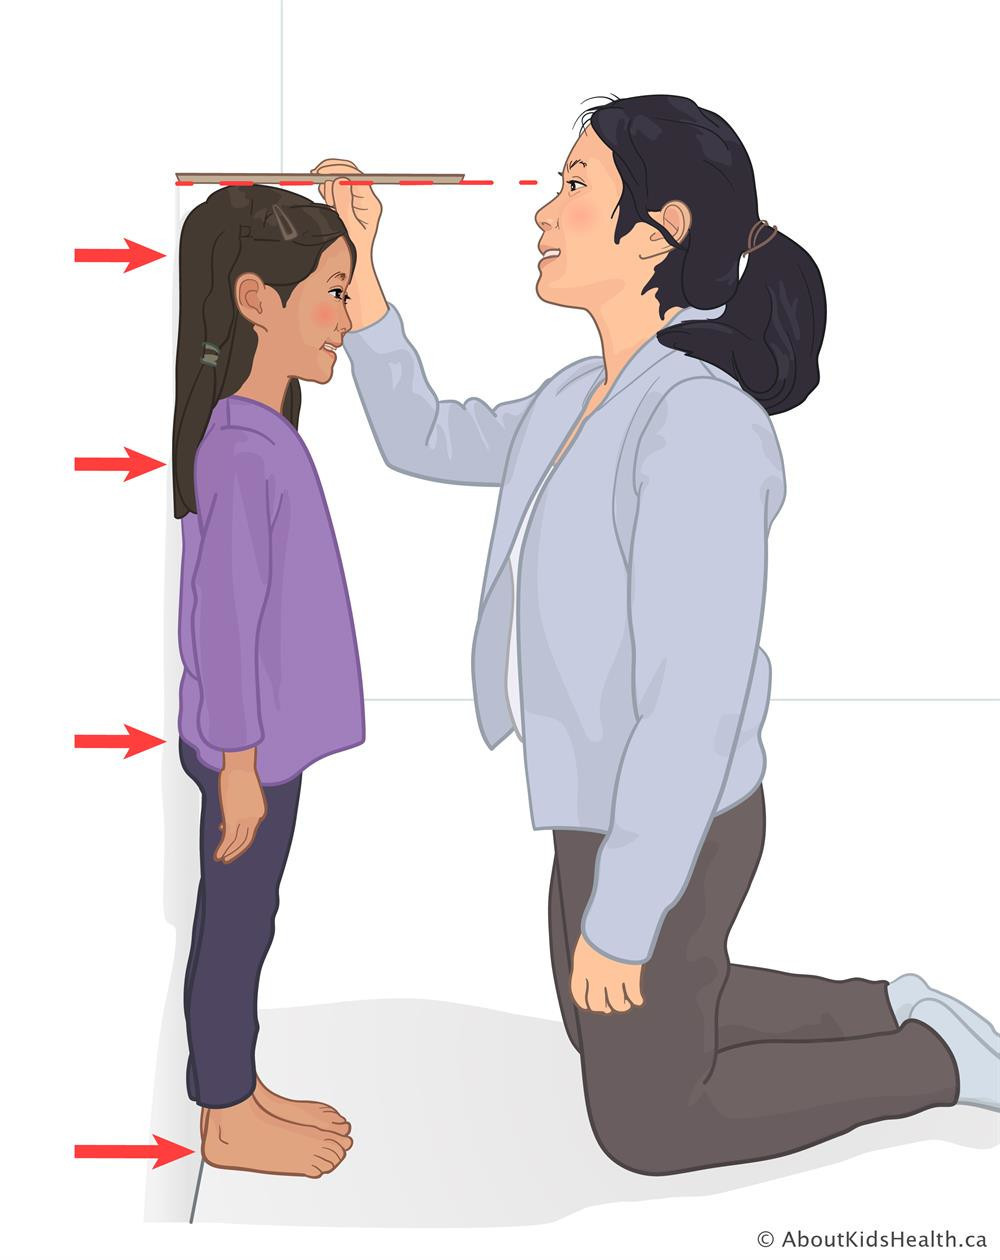
\includegraphics{D:/Usuarios/Juan/OneDrive/Documentos/010 Formación/001-Libro estadistica/01-imagenes/medida-altura-2.jpg}

}

\end{marginfigure}

Pero ¿y si la niña tiene una altura tal que el analista no puede
mantener una posición estable? El procedimiento real puede llegar a ser
mucho más complejo, tal como vemos en el último gráfico, que proviene de
un documento médico de la Organización Mundial de la Salud, en donde la
correcta estimación del peso y altura de los niños es fundamental para
determinar su estado de salud nutricional, y por lo tanto es necesario
minimizar el riesgo de errores de medida, garantizando que todos los
analistas realizan correctamente el mismo procedimiento aunque estén en
diferentes ubicaciones y en momentos diferentes:

\begin{marginfigure}

{\centering 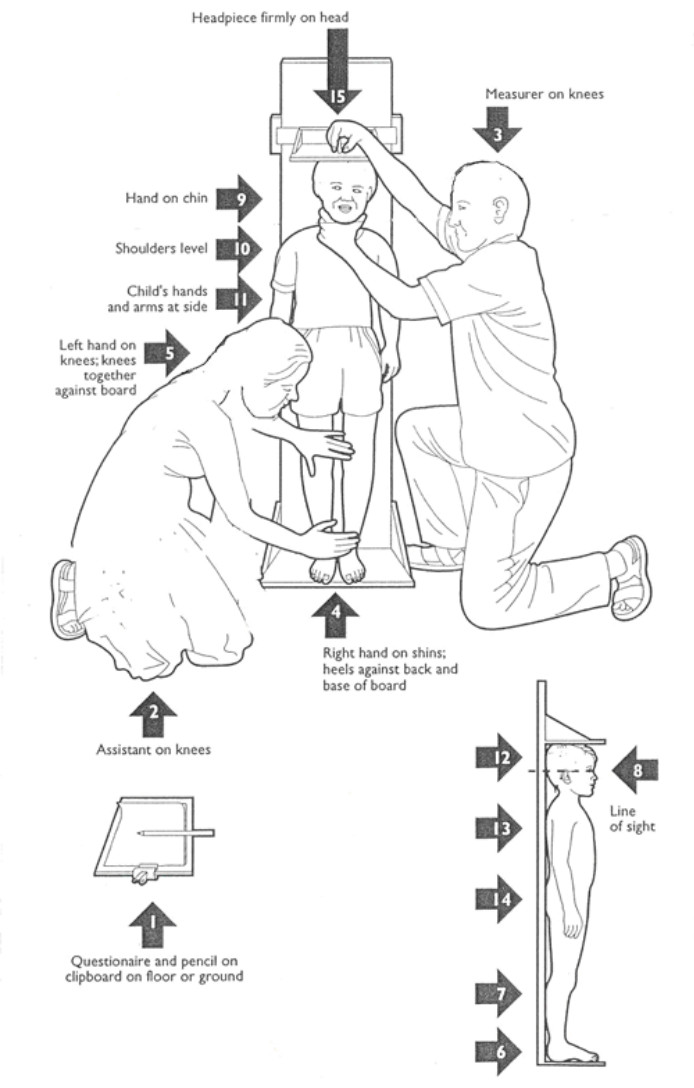
\includegraphics{D:/Usuarios/Juan/OneDrive/Documentos/010 Formación/001-Libro estadistica/01-imagenes/malnutrition-4.jpg}

}

\end{marginfigure}

EL procedimiento de la OMS ha estimado que es necesario que sean dos los
analistas que realizan la medida, utilizando un aparato especialmente
diseñado para ello, y que utiliza una pieza para ajustar a la cabeza de
manera que la posición de lectura no esté sometida al error de la
posición del analista que realiza la medida.

La descripción del procedimiento de análisis, junto con el detalle de
los instrumentos necesarios y sus homologaciones requeridas, constituye
lo que se conoce como \emph{método analítico}. El analista o analistas
deberán estudiar este \emph{método analítico} para estar seguros de que
son capaces de llevarlo a la práctica sin error.

Veremos en un apartado posterior que cada uno de estos elementos dan
lugar a un tipo de error concreto, que son principalmente dos: los
debidos al analista y los debidos al procedimiento (incluyendo aquí los
errores instrumentales) Veremos cómo evaluar la magnitud de cada uno de
estos errores y la forma de establecer un plan de trabajo para
reducirlos, mejorando así la calidad de nuestras medidas.

\hypertarget{la-precisiuxf3n-analuxedtica}{%
\section{La precisión analítica}\label{la-precisiuxf3n-analuxedtica}}

\hypertarget{anuxe1lisis-de-repetibilidad-y-reproducibilidad-grr-analysis}{%
\section{\texorpdfstring{Análisis de repetibilidad y reproducibilidad
(\emph{GR\&R
analysis})}{Análisis de repetibilidad y reproducibilidad (GR\&R analysis)}}\label{anuxe1lisis-de-repetibilidad-y-reproducibilidad-grr-analysis}}

\hypertarget{round-only-on-the-final-calculation-resultedit}{%
\subsection{\texorpdfstring{Round only on the final calculation
result{[}\href{https://en.wikipedia.org/w/index.php?title=Significant_figures\&action=edit\&section=14}{edit}{]}}{Round only on the final calculation result{[}edit{]}}}\label{round-only-on-the-final-calculation-resultedit}}

When performing multiple stage calculations, do not round intermediate
stage calculation results; keep as many digits as is practical (at least
one more digit than the rounding rule allows per stage) until the end of
all the calculations to avoid cumulative rounding errors while tracking
or recording the significant figures in each intermediate result. Then,
round the final result, for example, to the fewest number of significant
figures (for multiplication or division) or leftmost last significant
digit position (for addition or subtraction) among the inputs in the
final
calculation.{[}\href{https://en.wikipedia.org/wiki/Significant_figures\#cite_note-15}{15{]}}

\begin{itemize}
\tightlist
\item
  (2.3494 + 1.345) × 1.2 = 3.6944 × 1.2 = 4.43328 ≈ 4.4.
\item
  (2.3494 × 1.345) + 1.2 = 3.159943 + 1.2 = 4.359943 ≈ 4.4.
\end{itemize}

\hypertarget{precision-of-measuring-tools-and-significant-figures}{%
\section{Precision of Measuring Tools and Significant
Figures}\label{precision-of-measuring-tools-and-significant-figures}}

\href{https://courses.lumenlearning.com/atd-austincc-physics1/chapter/1-3-accuracy-precision-and-significant-figures/}{Accuracy,
Precision, and Significant Figures \textbar{} Physics
(lumenlearning.com)}

An important factor in the accuracy and precision of measurements
involves the precision of the measuring tool. In general, a precise
measuring tool is one that can measure values in very small increments.
For example, a standard ruler can measure length to the nearest
millimeter, while a caliper can measure length to the nearest 0.01
millimeter. The caliper is a more precise measuring tool because it can
measure extremely small differences in length. The more precise the
measuring tool, the more precise and accurate the measurements can be.

When we express measured values, we can only list as many digits as we
initially measured with our measuring tool. For example, if you use a
standard ruler to measure the length of a stick, you may measure it to
be 36.7 cm. You could not express this value as 36.71 cm because your
measuring tool was not precise enough to measure a hundredth of a
centimeter. It should be noted that the last digit in a measured value
has been estimated in some way by the person performing the measurement.
For example, the person measuring the length of a stick with a ruler
notices that the stick length seems to be somewhere in between 36.6 cm
and 36.7 cm, and he or she must estimate the value of the last digit.
Using the method of significant figures, the rule is that \textbf{the
last digit written down in a measurement is the first digit with some
uncertainty}. In order to determine the number of significant digits in
a value, start with the first measured value at the left and count the
number of digits through the last digit written on the right. For
example, the measured value 36.7cm has three digits, or significant
figures. Significant figures indicate the precision of a measuring tool
that was used to measure a value.

\hypertarget{la-mano-del-quesero}{%
\subsection{La ``mano del quesero''}\label{la-mano-del-quesero}}

Comparar pros y contras de la práctica basada en la experiencia con la
práctica basada ne el método y la cuantificación

\begin{itemize}
\tightlist
\item
  subjetividad
\item
  pérdida de conocimiento si el \emph{experto} deja la empresa
\end{itemize}

\hypertarget{muxe9todo-cientifico}{%
\subsection{Método cientifico}\label{muxe9todo-cientifico}}

Algoritmos - recetas cocina- DMAIC - método cientifico

Montgomery 1.1

\bookmarksetup{startatroot}

\hypertarget{el-control-estaduxedstico-de-procesos}{%
\chapter{El control estadístico de
procesos}\label{el-control-estaduxedstico-de-procesos}}

\hypertarget{la-mejora-de-la-calidad-y-el-control-estaduxedstico-de-procesos}{%
\section{La mejora de la calidad y el control estadístico de
procesos}\label{la-mejora-de-la-calidad-y-el-control-estaduxedstico-de-procesos}}

\hypertarget{introducciuxf3n-a-los-gruxe1ficos-de-control}{%
\section{Introducción a los gráficos de
control}\label{introducciuxf3n-a-los-gruxe1ficos-de-control}}

\hypertarget{causas-comunes-y-causas-especiales-de-variaciuxf3n}{%
\subsection{Causas comunes y causas especiales de
variación}\label{causas-comunes-y-causas-especiales-de-variaciuxf3n}}

\hypertarget{variaciuxf3n-a-corto-plazo-y-variaciuxf3n-a-largo-plazo}{%
\subsection{Variación a corto plazo y variación a largo
plazo}\label{variaciuxf3n-a-corto-plazo-y-variaciuxf3n-a-largo-plazo}}

\hypertarget{la-capacidad-de-un-proceso}{%
\section{La capacidad de un proceso}\label{la-capacidad-de-un-proceso}}

\hypertarget{ejemplo-establecer-las-especificaciones-de-un-producto}{%
\section{Ejemplo: establecer las especificaciones de un
producto}\label{ejemplo-establecer-las-especificaciones-de-un-producto}}

\bookmarksetup{startatroot}

\hypertarget{diseuxf1o-de-experimentos}{%
\chapter{Diseño de experimentos}\label{diseuxf1o-de-experimentos}}

¿La aspirina reduce el riesgo de infarto? ¿Una marca de abono es más
eficaz para el cultivo de rosas que otra? ¿El cansancio es tan peligroso
para un conductor como la influencia del alcohol? Este tipo de preguntas
se responden con experimentos aleatorios.

El propósito de un experimento es investigar la relación entre dos o más
variables. Cuando una variable provoca un cambio en otra, llamamos a la
primera variable la \textbf{variable independiente} o
\textbf{explicativa}. La variable afectada se llama \textbf{variable
dependiente} o \textbf{variable de respuesta}: estímulo, respuesta. En
un experimento aleatorio, el investigador manipula los valores de la
variable explicativa y mide los cambios resultantes en la variable de
respuesta. Los diferentes valores de la variable explicativa se
denominan \textbf{tratamientos}. Una \textbf{unidad experimental} es un
único objeto o persona que se va a medir.

Supongamos que usted quiere investigar la eficacia de la vitamina E en
la prevención de enfermedades. Usted recluta a un grupo de sujetos y les
pregunta si toman regularmente vitamina E. Observa que los sujetos que
toman vitamina E, en promedio, presentan una salud mejor que quienes no
la toman. ¿Esto prueba que la vitamina E es eficaz en la prevención de
enfermedades? No es así. Hay muchas diferencias entre los dos grupos
comparados, además del consumo de vitamina E. Las personas que toman
vitamina E con regularidad suelen tomar otras medidas para mejorar su
salud: ejercicio, dieta, otros suplementos vitamínicos, elección de no
fumar, etc. Cualquiera de estos factores podría estar influyendo en la
salud. Como se ha descrito, este estudio no demuestra que la vitamina E
sea la clave para la prevención de enfermedades.

Las variables adicionales que pueden enturbiar un estudio se denominan
\textbf{variables ocultas}. Para demostrar que la variable explicativa
provoca un cambio en la variable de respuesta, es necesario aislar la
variable explicativa. La investigadora debe diseñar su experimento de
forma que solo haya una diferencia entre los grupos que se comparan: los
tratamientos previstos. Esto se consigue mediante la \textbf{asignación
aleatoria} de unidades experimentales a grupos de tratamiento. Cuando
los sujetos se asignan a los tratamientos de forma aleatoria, todas las
variables ocultas potenciales se reparten por igual entre los grupos. En
este punto, la única diferencia entre los grupos es la impuesta por el
investigador. Los diferentes resultados medidos en la variable de
respuesta, por tanto, deben ser una consecuencia directa de los
diferentes tratamientos. De este modo, un experimento puede demostrar
una conexión causa-efecto entre las variables explicativas y las de
respuesta.

El poder de la sugestión puede tener una importante influencia en el
resultado de un experimento. Los estudios han demostrado que la
expectativa del participante en el estudio puede ser tan importante como
el medicamento real. En un estudio sobre fármacos que mejoran el
desempeño, los investigadores señalaron:

\begin{quote}
Los resultados mostraron que creer que se había tomado la sustancia
provocaba tiempos de {[}desempeño{]} casi tan rápidos como los asociados
al consumo del propio fármaco. Por el contrario, la toma del fármaco sin
conocimiento no produjo un aumento significativo del
desempeño.{[}\^{}1{]} .
\end{quote}

Cuando la participación en un estudio provoca una respuesta física del
participante, es difícil aislar los efectos de la variable explicativa.
Para contrarrestar el poder de la sugestión, los investigadores
reservaron un grupo de tratamiento como \textbf{grupo de control} . Este
grupo recibe un tratamiento \textbf{placebo}, es decir, un tratamiento
que no puede influir en la variable de respuesta. El grupo de control
ayuda a los investigadores a equilibrar los efectos de estar en un
experimento con los efectos de los tratamientos activos. Por supuesto,
si usted participa en un estudio y sabe que está recibiendo una píldora
que no contiene ningún medicamento real, entonces el poder de la
sugestión ya no es un factor. Que un experimento aleatorio sea
\textbf{ciego} preserva el poder de la sugestión. Cuando una persona
participa en un estudio de investigación ciego, no sabe quién recibe el
tratamiento activo y quién el placebo. Un \textbf{experimento doble
ciego} es aquel en el que tanto los sujetos como los investigadores que
participan en él no conocen la información del fármaco.

\hypertarget{experimentos-factoriales}{%
\section{Experimentos factoriales}\label{experimentos-factoriales}}

No un factyor de cada vez - explciar interaccion

\bookmarksetup{startatroot}

\hypertarget{la-calidad-y-la-mejora-de-la-calidad}{%
\chapter{La calidad y la mejora de la
calidad}\label{la-calidad-y-la-mejora-de-la-calidad}}

\hypertarget{six-sigma-y-mejora-de-la-calidad}{%
\section{Six Sigma y mejora de la
calidad}\label{six-sigma-y-mejora-de-la-calidad}}

\hypertarget{definir-un-problema-opex-lean-sixsigma-16}{%
\section{Definir un problema {[}OPEX Lean SixSigma
\#16{]}}\label{definir-un-problema-opex-lean-sixsigma-16}}

\hypertarget{cuxf3mo-es-una-buena-definiciuxf3n-de-un-problema}{%
\subsection{¿Cómo es una buena definición de un
problema?}\label{cuxf3mo-es-una-buena-definiciuxf3n-de-un-problema}}

\begin{itemize}
\tightlist
\item
  Breve
\item
  Evitar lenguaje técnico: debes ser capaz de explicarlo a cualquier
  persona de la organización usando términos sencillos
\item
  Cuantificar el problema, usando los datos disponibles
\item
  Integra y explica el coste real del problema, para justificar la
  necesidad del análisis. Puedes relacionarlo con los \emph{costes de no
  calidad}
\item
  Define el ámbito del problema: usa los términos que sean necesarios
  para delimitarlo con precisión.
\item
  La definición de un problema debe conseguir formularlo de forma que
  sea específico, medible, realizable, relevante y acotado en el tiempo
  (plazo)
\end{itemize}

\hypertarget{estrategia-de-resolucion-de-problemas}{%
\section{Estrategia de resolucion de
problemas}\label{estrategia-de-resolucion-de-problemas}}

\hypertarget{r4ds}{%
\section{R4DS}\label{r4ds}}

Fuente: R4DS

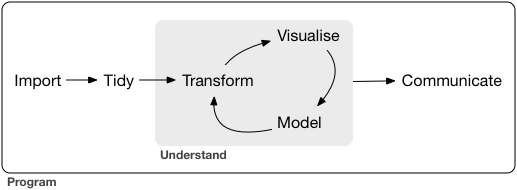
\includegraphics{01-imagenes/data-science.png}

\hypertarget{dmaic---sixsigma}{%
\section{DMAIC - SixSigma}\label{dmaic---sixsigma}}

\hypertarget{el-papel-de-los-muxe9todos-estaduxedsticos-en-la-mejora-six-sigma}{%
\section{El papel de los métodos estadísticos en la mejora Six
Sigma}\label{el-papel-de-los-muxe9todos-estaduxedsticos-en-la-mejora-six-sigma}}

\bookmarksetup{startatroot}

\hypertarget{anexo-recetario-de-muxe9todos}{%
\chapter{Anexo: Recetario de
métodos}\label{anexo-recetario-de-muxe9todos}}

\bookmarksetup{startatroot}

\hypertarget{bibliografuxeda}{%
\chapter*{Bibliografía}\label{bibliografuxeda}}
\addcontentsline{toc}{chapter}{Bibliografía}

\markboth{Bibliografía}{Bibliografía}

\hypertarget{refs}{}
\begin{CSLReferences}{1}{0}
\leavevmode\vadjust pre{\hypertarget{ref-science2015}{}}%
Buck, Stuart. 2015. {«Solving reproducibility»}. \emph{Science} 348
(6242): 1403.
\url{https://www.science.org/doi/full/10.1126/science.aac8041}.

\leavevmode\vadjust pre{\hypertarget{ref-ferrero2018}{}}%
Ferrero, Rosana. 2018. {«Los errores de Reinhart \& Rogoff: R y la
reproducibilidad»}. 2018.
\url{https://www.maximaformacion.es/blog-dat/los-errores-de-reinhart-rogo/}.

\leavevmode\vadjust pre{\hypertarget{ref-wickham2017}{}}%
Hadley Wickham, Garret Grolemund. 2017. \emph{R for Data Science}. 1005
Gravenstein Highway North, Sebastopol, CA95472: O'Reilly Media Inc.
\url{https://r4ds.had.co.nz/index.html}.

\leavevmode\vadjust pre{\hypertarget{ref-ryssdal2013}{}}%
Ryssdal, Karl. 2013. {«The Excel mistake heard round the world»}. 2013.
\url{https://www.marketplace.org/2013/04/17/economy/excel-mistake-heard-round-world/}.

\leavevmode\vadjust pre{\hypertarget{ref-sadler2017}{}}%
Sadler, Jesse. 2017. {«Excel vs R: A Brief Introduction to R»}. 2017.
\url{https://www.jessesadler.com/post/excel-vs-r/}.

\leavevmode\vadjust pre{\hypertarget{ref-wickham2014}{}}%
Wickham, Hadley. 2014. {«Tidy Data»}. \emph{Journal od Statistical
Software} 59 (10): 1-23. \url{https://doi.org/10.18637/jss.v059.i10}.

\end{CSLReferences}



\end{document}
